\documentclass[lettersize,journal]{IEEEtran}
\usepackage[T1]{fontenc}
\usepackage[utf8]{inputenc}
\usepackage{amsmath,amssymb,amsfonts}
\usepackage{tikz}                                                          % you want to use the \thanks command
\usepackage[T1]{fontenc}
\usepackage[utf8]{inputenc}
\usepackage{xcolor,colortbl}
\usepackage{subcaption}
\graphicspath{ {images/} } 
\usepackage{blindtext}
\usepackage{subfiles}
\usepackage{algorithm}
\usepackage{algpseudocode}
\usepackage{multicol}
% \usepackage{float}
\usepackage{stfloats}
\usepackage{array}
%\usepackage[maxfloats=256]{morefloats}
%\maxdeadcycles=15000
\usepackage{url}
\usepackage{diagbox}
\usepackage{flushend}
\usepackage{lipsum}
\usepackage[verbose]{placeins} 
\usepackage{multirow}
\usetikzlibrary{arrows.meta, positioning}
\usepackage{subcaption}
% \PassOptionsToPackage{svgnames}{xcolor}
\hyphenation{op-tical net-works semi-conduc-tor IEEE-Xplore}
% updated with editorial comments 8/9/2021
\newtheorem{lemma}{Lemma}
% \newtheorem{problem}{Problem}
\newcommand{\problemtitle}[2]{%
  \parbox{\linewidth}{\centering\textbf{#1} \\ \textbf{#2}}%
}
\newtheorem{problem}{\textbf{Problem}}
\newtheorem{proposition}{Proposition}
\newtheorem{remark}{Remark}
\newtheorem{theorem}{\normalfont\textbf{Theorem}}
\newtheorem{corollary}{\normalfont\textbf{Corollary}}
\newcommand{\mycomment}[1]{}
\newcommand{\algrule}[1][.2pt]{\par\vskip.5\baselineskip\hrule height #1\par\vskip.5\baselineskip}
\newcolumntype{C}[1]{>{\centering\arraybackslash}p{#1}}
\newcolumntype{M}[1]{>{\centering\arraybackslash}m{#1}}
\let\labelindent\relax  % Redefine before loading enumitem
\usepackage{enumitem}
\newcommand{\purplecircle}{\textcolor{blue}{\textbullet}}
\newcommand{\largepurplecircle}{\textcolor{blue}{\scalebox{1.5}{$\bullet$}}}
\newcommand{\CRD}{$\text{C}_{\text{R}} \text{D }$}
\newcommand{\qedwhite}{\hfill \ensuremath{\Box}}
% \usepackage{semantic}

\begin{document}

% \title{On Transport Justice in Bicycle Network Design: \\ Balancing Safety and Car Impacts}
% \title{Balancing Safety of Cyclists and Impact on Vehicular Flow}
\title{Justice-informed Cycling Infrastructure Upgrade\\
via Multi-modal Bi-level Optimization}

\author{Manuel Campero Jurado$^{1}$, Carlos Canudas-de-Wit$^{2}$, Giovanni De Nunzio$^{3}$, Mauro Salazar$^{4}$% <-this % stops a space
% \thanks{*This work was not supported by any organization}% <-this % stops a space
%\thanks{We thank Dr.\ I.\ New for proofreading this paper. M.\ Campero Jurado visited Eindhoven University of Technology with the support of an outgoing mobility grant IDEX from the Univ.\ Grenoble Alpes.}
\thanks{$^{1}$IFP Energies nouvelle, Rueil Malmaison, France, {\footnotesize \textit{manuel.campero-jurado@ifpen.fr}} (\textit{Corresponding author})}
\thanks{$^{2}$Univ. Grenoble Alpes, Inria, CNRS, Grenoble INP, GIPSA-Lab, 38000 Grenoble, France,
        {\footnotesize \textit{carlos.canudas-de-wit@gipsa-lab.fr}}}%
\thanks{$^{3}$IFP Energies nouvelles,
Rond-point de l’échangeur de Solaize, BP 3, 69360 Solaize, France,
        {\footnotesize \textit{giovanni.de-nunzio@ifpen.fr}}}%
\thanks{$^{4}$Eindhoven University of Technology, 5600 MB, Eindhoven, The Netherlands,
{\footnotesize \textit{m.r.u.salazar@tue.nl}}}%
}


% \author{IEEE Publication Technology,~\IEEEmembership{Staff,~IEEE,}
%         % <-this % stops a space
% \thanks{This paper was produced by the IEEE Publication Technology Group. They are in Piscataway, NJ.}% <-this % stops a space
% \thanks{Manuscript received April 19, 2021; revised August 16, 2021.}}

% % The paper headers
% \markboth{Journal of \LaTeX\ Class Files,~Vol.~14, No.~8, August~2021}%
% {Shell \MakeLowercase{\textit{et al.}}: A Sample Article Using IEEEtran.cls for IEEE Journals}

% \IEEEpubid{0000--0000/00\$00.00~\copyright~2021 IEEE}
% Remember, if you use this you must call \IEEEpubidadjcol in the second
% column for its text to clear the IEEEpubid mark.

\maketitle

\begin{abstract}
% Promoting cycling as a sustainable mode of transport requires infrastructure that improves safety. At the same time, mode improvements may negatively affect motorized traffic. This paper presents a multi-modal bi-level optimization framework that integrates transport justice principles into cycling infrastructure planning. The framework couples a bicycle flow model based on shortest-path assignment with a surrogate machine learning model that efficiently approximates car traffic equilibrium, enabling realistic city-scale analysis. The framework also captures induced modal shifts from cars to bicycles due to cycling infrastructure improvements.

% Two complementary formulations are introduced: a utilitarian model minimizing total system travel time and cyclist exposure, and a sufficientarian model maximizing the share of users above safety and accessibility thresholds. Applied to the Grenoble network, the results show that both approaches substantially increase safety and accessibility fairness, with the sufficientarian strategy achieving the most balanced outcomes—reducing cyclist exposure and safety-path insufficiency while mitigating the negative accessibility impacts on drivers. Overall, the proposed approach demonstrates that just, low-carbon transport planning can improve safety and fairness without compromising efficiency.
Promoting cycling requires an infrastructure that better protects cyclists from motor traffic, but reallocating road space to bicycles can increase car travel times. This creates a trade-off between reducing cyclists' exposure to motorized traffic and maintaining network efficiency, as well as a distributional question: Should interventions maximize aggregate benefits or prioritize users facing insufficient conditions?

We address these questions through an integrated bi-level transport-network optimization framework for jointly designing cycling and car networks. It combines a safety-adjusted bicycle assignment model, a behavioral modal-shift model, and a machine-learning surrogate for car user equilibrium. We consider two justice-oriented formulations: a utilitarian model minimizing cyclist exposure and total system travel time, and a sufficientarian model reducing cycling-path insufficiency and trips exceeding a travel-time threshold. The former emphasizes aggregate performance, while the latter prioritizes users facing insufficient path-protection or travel-time conditions. Applied to Grenoble, both formulations reduce cyclist exposure while limiting increases in car travel times. The sufficientarian approach provides the most balanced outcome, demonstrating that path and travel-time sufficiency can be improved without sacrificing aggregate transport efficiency.


% Applied to the Grenoble network, both formulations reduce cyclist exposure and improve exposure-based path sufficiency while limiting increases in car travel times. The sufficientarian formulation provides the most balanced distribution of outcomes, reducing cycling-path and bicycle-trip insufficiency while limiting increases in driver trip insufficiency. These results show that cycling infrastructure can support low-carbon mobility while balancing cyclist protection, distributive justice, and transport efficiency.


\end{abstract}

\begin{IEEEkeywords}
Multi-modal network optimization, transport justice, mode-shift modeling, bi-level optimization and sustainable transportation.
\end{IEEEkeywords}

\section{Introduction}
Cycling offers major health, environmental, and economic benefits, including improved public health, reduced congestion, and lower emissions~\cite{garrard2012health, gotschi2016cycling}.
Consequently, several cities worldwide promote cycling as a sustainable transport mode, especially for short trips.
However, safety and comfort remain key barriers to widespread adoption~\cite{fishman2012barriers}.
Physically separated cycling facilities have been shown to enhance safety and increase ridership~\cite{lawrence2018cyclist, pucher2011walking}, yet reallocating road space to bicycles can reduce vehicle capacity and increase car travel times.
This trade-off underscores the need for planning tools that improve cycling safety while balancing multi-modal traffic performance (see Fig.~\ref{multi_network} for
the existing bicycle and road networks in Grenoble).

From a societal perspective, cycling investments also raise distributional concerns. Building on transport justice theory~\cite{martens2017transport}, two perspectives are central: a utilitarian-efficiency approach that maximizes aggregate welfare by minimizing cyclist exposure and total system travel time, and a sufficientarian approach that seeks to reduce cycling-path insufficiency and trip insufficiency, i.e., cases where users fall below an acceptable exposure-based protection level or exceed a reasonable travel-time threshold. Incorporating these principles into network design requires models capable of capturing modal shifts, traffic equilibrium, and cycling-flow redistribution under infrastructure upgrades.


\begin{figure}[t]
\vspace{0.2cm}
  \centering
 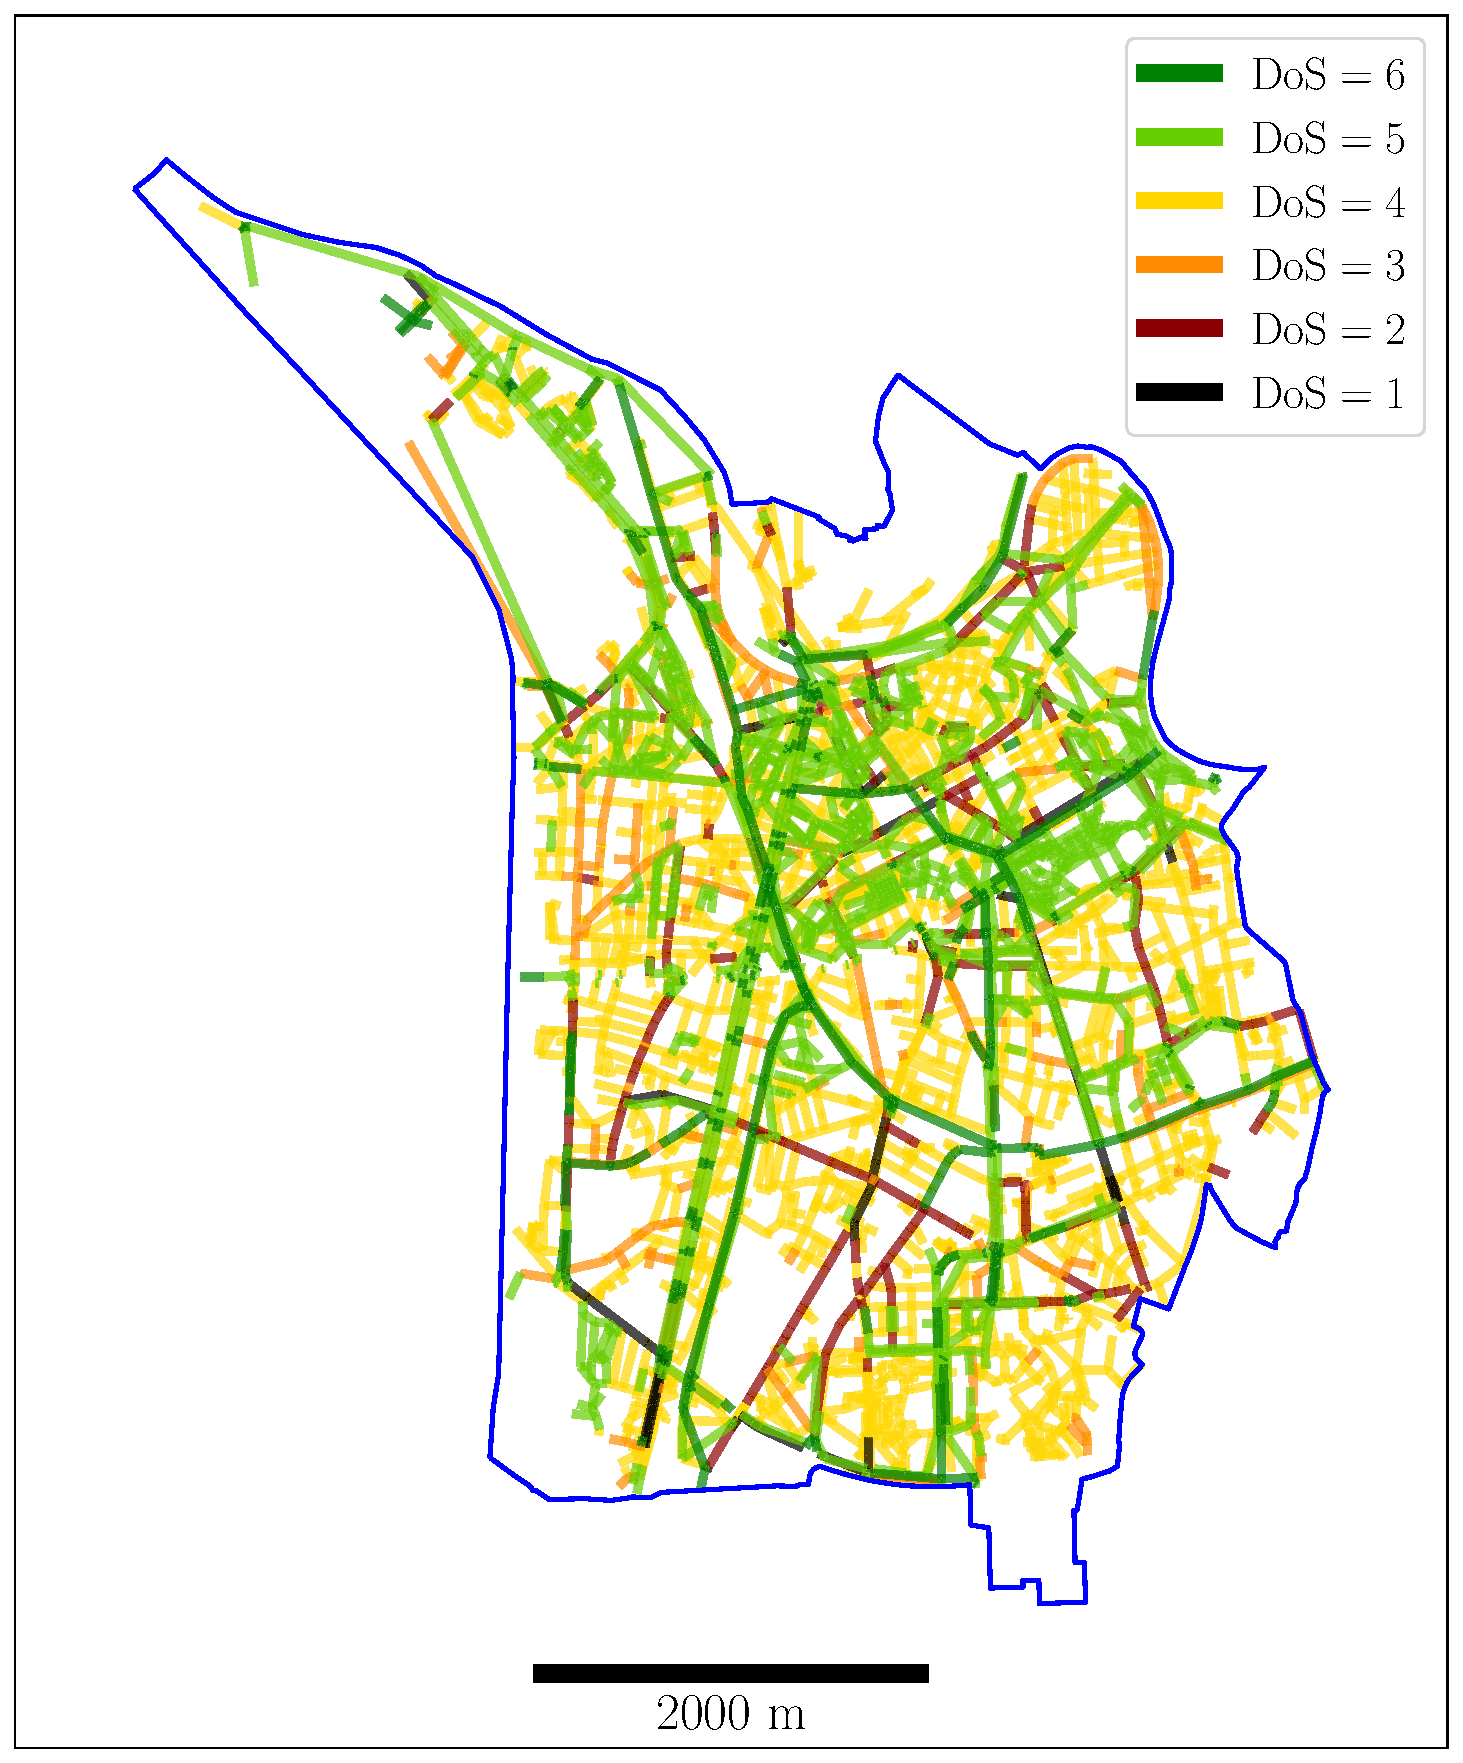
\includegraphics[width=0.48\linewidth]{Images/Grenoble_bikes_network.pdf}
 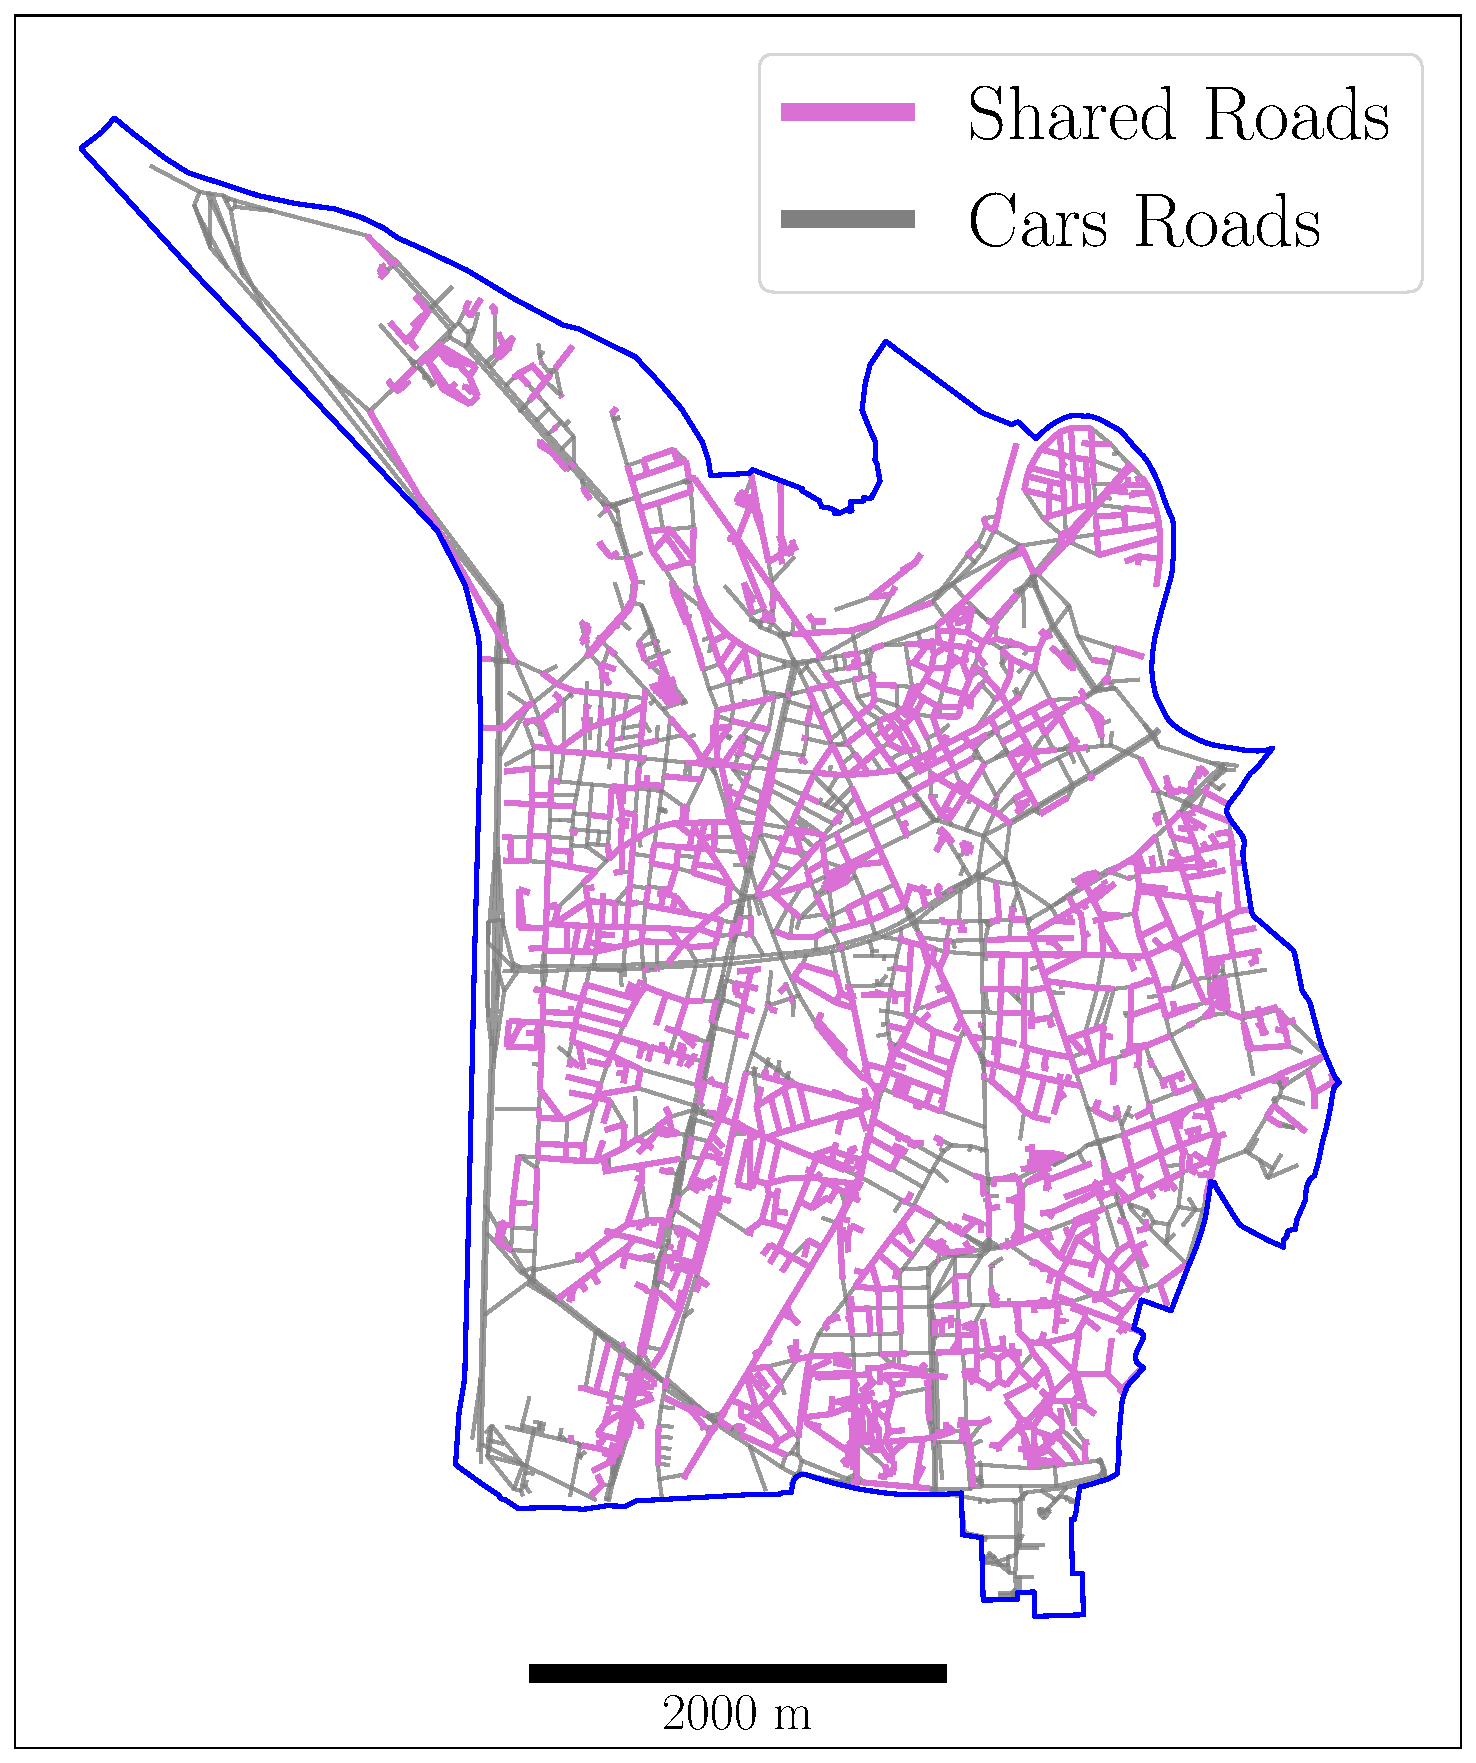
\includegraphics[width=0.485\linewidth]{Images/Grenoble_cars_network.pdf}
  \caption{\footnotesize Multi-modal transportation network of Grenoble, France. \textit{Left:} Cycling infrastructure classified by degree of separation (DoS) of bike lanes, ranging from 1 (least separated) to 6 (fully separated). \textit{Right:} Road network for cars, including links shared with bicycles.}
  \label{multi_network}
\end{figure}

% \subsection{Literature Review} 

% Our work draws on three primary domains: cycling network optimization, the analysis of modal shifts in urban mobility and transport justice.

% \textit{Cycling Network Optimization}: Research on cycling network planning addresses objectives such as usage, connectivity, safety, and multi-modal impacts. Early studies optimized network design to increase bike-lane use measured by the total distance traveled on designated facilities as a proxy for infrastructure utilization and accessibility, while improving topological connectivity \cite{mesbah2012bilevel,smith2012mathematical,duthie2014optimization}. Subsequent works examined benefit–cost trade-offs and proposed budget-constrained heuristics to guide investment decisions \cite{paulsen2023societally,shui2019optimization,folco2023data}. More recent graph-theoretic approaches explicitly targeted safety by reconfiguring networks toward higher protection levels, though they often overlook how improvements are distributed across users and regions \cite{2024graphbased}. In parallel, multi-modal interactions have been modeled through bi-level formulations that balance cycling upgrades with car accessibility \cite{mesbah2012bilevel,smith2012mathematical,wiedemann2025bike} and heuristic methods that capture traffic disruption under lane reallocation \cite{mahfouz2023road}. Overall, most approaches emphasize efficiency or travel time. Safety is sometimes considered at an aggregate level, but the fairness of how safety and accessibility gains are distributed, who benefits, where, and by how much remains largely underexplored.

% \textit{Modal Shift in Urban Mobility:}  Utility cycling has become an increasingly credible alternative to driving in urban areas, although cars still dominate public space and policy agendas \cite{cox2020theorising}. Infrastructure quality plays a central role in enabling this shift: cyclists consistently prefer separation from motorized traffic, while poor pavement conditions discourage cycling \cite{buehler2016bikeway}. Thus, the design, continuity, and inclusiveness of cycling infrastructure are key determinants of bikeability, requiring diverse and connected facilities that serve different users and trip purposes \cite{cox2020politics}. At the behavioral level, agent-based models simulate individual mobility decisions, showing that improvements in cycling safety or reductions in car comfort can drive meaningful shifts toward active transport \cite{adam2024agent}. Empirical studies indicate that many car trips could be replaced by low-carbon or active modes without significant increases in travel time \cite{monzon2006measure,monzon2011potential}. Recent computational frameworks use smartphone-based data to estimate modal-shift potential and emission reductions \cite{bagheri2020computational,bagheri2020analysis}. However, most of these studies do not explicitly classify cycling infrastructure by safety level, nor do they analyze how upgrades between levels affect the modal shift from cars to bicycles.


% \textit{Transport justice:} Traditional transport models have mainly adopted a utilitarian perspective~\cite{mill2016utilitarianism}, aiming to maximize total welfare by improving aggregate outcomes, regardless of how benefits are distributed. In this view, inequalities are acceptable as long as they increase overall utility~\cite{binmore1998egalitarianism}, which means that policies that disadvantage minorities or favour travellers with higher values of time can still be considered ``optimal''~\cite{pereira2017distributive}. As an alternative, Rawls’ egalitarian theory~\cite{rawls2017theory,rawls1971theory} and the capabilities approach have been proposed as more suitable foundations for transport justice, since they emphasize fair opportunities and attention to the least advantaged. Building on these ideas, Martens~\cite{martens2017transport} introduces a sufficientarian perspective for transport, arguing that justice should focus on guaranteeing a minimum level of accessibility for everyone, while accessibility above this threshold may be left to market-based or self-financing mechanisms. This has led to the use of accessibility sufficiency indices as core indicators of justice in transport planning~\cite{martens2022equity}, and has been extended to multi-modal settings~\cite{salazar2024accessibility} and complemented by capabilities-based analyzes across different contexts~\cite{amorim2024comparing}. However, with the exception of \cite{salazar2024accessibility, salazar2025mobilizing}, most of this work remains largely evaluative: it identifies where and for whom accessibility is insufficient, but does not offer operational tools to design or optimize networks in line with these principles. To date, only \cite{jurado2025transport} applies principles of justice to the optimization of a cycling network by targeting sufficient safety along paths, but it does not account for the impact on car travel times through potential reductions in road capacity. In conclusion, to the best of the authors’ knowledge, there is still no prescriptive, operational framework that optimizes multi-modal (bike + car) networks in line with both utilitarian and sufficientarian principles, while simultaneously reducing cyclist safety risks and explicitly accounting for car travel-time accessibility impacts arising from road capacity reductions and induced mode shifts that modify origin–destination demand for both cyclists and drivers.


% \textit{Statement of Contributions:} 
% This paper makes three main contributions. 
% First, we propose a multi-modal bi-level optimization framework for the joint design of cycling and car networks that embeds both utilitarian and sufficientarian principles to balance safety, accessibility fairness, and travel-time efficiency.  Second, we link infrastructure design to travel behavior by combining a behavioral mode-choice and modal-shift model with a surrogate machine-learning model that efficiently approximates car user equilibrium at the city scale. Third, we demonstrate the practical relevance of this framework on the Grenoble network, showing that substantial improvements in cyclist safety and accessibility fairness can be achieved with limited negative impacts on car travel times. More specifically, building on previous work on cycling infrastructure classification~\cite{jurado2025safety}, we exploit the notion of safety-adjusted cycling distance to model bicycle flows through a shortest-path assignment that accounts for infrastructure type and degree of segregation from motor traffic. 
% We then introduce a behavioral modal-shift model to estimate how car drivers transition to cycling following bike-lane upgrades, and couple it with a graph-based surrogate model that approximates user-equilibrium car flows. 
% Finally, we solve the resulting bi-level problems with two heuristic algorithms—a genetic algorithm and a modified connectivity-based method—highlighting how different justice-oriented formulations lead to distinct yet complementary network design strategies.


This paper presents a framework for multi-modal network planning that integrates these perspectives under budget constraints. The model accounts for induced modal shifts from cars to bicycles following cycling infrastructure upgrades, dynamically adjusting travel demand across modes. To capture car traffic responses efficiently, we employ a surrogate machine learning model that approximates user equilibrium flows, allowing realistic yet computationally tractable city-scale analyses. Two bi-level optimization formulations are then introduced: a utilitarian model that minimizes aggregate cyclist exposure and total system travel time, and a sufficientarian model that maximizes the number of cyclists exceeding a path-sufficiency threshold while minimizing the proportion of cyclists and drivers who do not meet a maximum travel time threshold.


% \subsection{Literature Review}

% Our work lies at the intersection of three main research areas: cycling network optimization, modal-shift modelling, and transport justice.

% \textit{Cycling network optimization:}
% Research on cycling network planning has considered objectives such as infrastructure use, connectivity, safety, investment efficiency, and interactions with other transport modes. Early studies formulated network design problems to increase the use of designated cycling facilities while improving connectivity and accessibility \cite{mesbah2012bilevel,smith2012mathematical,duthie2014optimization}. Subsequent works examined benefit--cost trade-offs and developed budget-constrained methods to support infrastructure investment decisions \cite{paulsen2023societally,shui2019optimization,folco2023data}. More recent graph-based approaches have explicitly addressed cyclist safety by identifying or upgrading links toward higher levels of protection \cite{2024graphbased}. Multi-modal formulations have also considered the effects of cycling improvements on car accessibility and traffic conditions \cite{mesbah2012bilevel,smith2012mathematical,wiedemann2025bike}, including the disruption caused by reallocating road capacity from cars to bicycles \cite{mahfouz2023road}. However, most approaches continue to emphasize aggregate measures of efficiency, connectivity, or safety, with limited attention to how the benefits and disadvantages of infrastructure interventions are distributed across users.

% \textit{Modal shift in urban mobility:}
% Cycling is increasingly recognized as a viable alternative to private cars for urban travel, although motorized transport continues to dominate road-space allocation and transport policies \cite{cox2020theorising}. The quality and continuity of cycling infrastructure strongly influence its attractiveness. Cyclists generally prefer facilities that provide separation from motor traffic, whereas poor pavement quality and discontinuous routes can discourage cycling \cite{buehler2016bikeway}. Consequently, connected and inclusive cycling networks are important for serving different users and trip purposes \cite{cox2020politics}.

% Behavioural and computational studies have examined how changes in infrastructure and travel conditions influence transport-mode choices. Agent-based models suggest that safer cycling conditions or reduced convenience for car travel can encourage shifts toward active mobility \cite{adam2024agent}. Empirical studies similarly indicate that many car trips could be replaced by active or low-carbon modes without substantial increases in travel time \cite{monzon2006measure,monzon2011potential}. Data-driven approaches have also been used to estimate modal-shift potential and the associated reduction in emissions \cite{bagheri2020computational,bagheri2020analysis}. Nevertheless, modal-shift models are rarely integrated directly into cycling network optimization. In particular, existing approaches seldom examine how upgrades between different infrastructure safety levels affect route choice and the demand for both cycling and car travel.

% \textit{Transport justice:}
% Traditional transport planning has largely followed a utilitarian perspective \cite{mill2016utilitarianism}, seeking to maximize aggregate welfare or system efficiency without necessarily considering how benefits and burdens are distributed. Under this perspective, inequalities may be accepted when they lead to a higher total utility \cite{binmore1998egalitarianism}, meaning that an intervention can be considered optimal even when some users receive few benefits or experience worse conditions \cite{pereira2017distributive}.

% Alternative theories, including Rawlsian egalitarianism \cite{rawls2017theory,rawls1971theory} and the capabilities approach, emphasize fair opportunities and the conditions experienced by disadvantaged users. Building on these ideas, Martens \cite{martens2017transport} proposes a sufficientarian perspective in which transport policy should first guarantee a minimum acceptable level of accessibility. This principle has motivated the development of accessibility-sufficiency indicators \cite{martens2022equity}, multi-modal applications \cite{salazar2024accessibility}, and capabilities-based analyses in different transport contexts \cite{amorim2024comparing}.

% Despite these developments, much of the transport-justice literature remains evaluative: it identifies inequalities or insufficient accessibility but does not directly determine how networks should be redesigned to improve these conditions. Recent studies have started to introduce justice principles into transport optimization \cite{salazar2024accessibility,salazar2025mobilizing,jurado2025transport}, but their integration with multi-modal infrastructure planning remains limited.

% Overall, existing research has made important advances in cycling network design, modal-shift analysis, and transport justice, but these areas remain only partially connected. There is still a need for a prescriptive framework that jointly considers cycling safety, car-network performance, travellers' behavioural responses, and the distribution of safety and accessibility outcomes. Such a framework is necessary to examine both the efficiency of cycling investments and whether their benefits and burdens are fairly distributed across transport users.

% \textit{Statement of Contributions:}
% This paper addresses this gap by proposing a multi-modal bi-level optimization framework for cycling infrastructure planning. Its overall contribution is to integrate cyclist safety, car accessibility, modal shift, and distributive justice within a common network design framework. Two complementary formulations are considered: a utilitarian formulation that prioritizes aggregate safety and travel-time outcomes, and a sufficientarian formulation that seeks to ensure that as many users as possible achieve acceptable levels of safety and accessibility.

% A preliminary version of this work was presented at the 2025 IEEE Conference on Decision and Control~\cite{jurado2025transport}. That paper compared utilitarian and sufficientarian formulations for the optimization of the cycling network, focusing on cyclist safety. However, it did not represent the car network or consider how cycling infrastructure interventions affect car accessibility. The present paper extends this preliminary work to a multi-modal setting by jointly considering bicycle and car users.

% More specifically, the paper makes three main contributions. First, we formulate a multi-modal bi-level network design problem that captures the trade-off between improving cycling safety and limiting negative effects on car travel times and accessibility. The utilitarian and sufficientarian formulations also make it possible to compare aggregate improvements with the provision of minimum acceptable conditions across users. Second, we connect infrastructure design with changes in travel behavior. Cycling flows are represented through a safety-adjusted shortest-path assignment based on infrastructure type and separation from motor traffic \cite{jurado2025safety}. A behavioral modal-shift model then estimates how cycling upgrades modify bicycle and car demand, while a graph-based machine-learning surrogate efficiently approximates car user-equilibrium conditions at the city scale. Third, we solve the resulting design problems using a genetic algorithm and a modified connectivity-based heuristic and evaluate the framework on the Grenoble network. The case study illustrates how utilitarian and sufficientarian principles lead to different but complementary infrastructure strategies and different balances among cyclist safety, accessibility fairness, modal shift, and car travel-time efficiency.

\subsection{Literature Review}

Our work lies at the intersection of three main research areas: cycling network optimization, modal-shift modeling, and transport justice.

\textit{Cycling network optimization:}
Research on cycling network planning has considered objectives such as infrastructure use, connectivity, safety-related conditions, investment efficiency, and interactions with other transport modes. Early studies formulated network design problems to increase the use of designated cycling facilities while improving connectivity and expand the cycling bike lanes \cite{mesbah2012bilevel,smith2012mathematical,duthie2014optimization}. Subsequent studies by Paulsen et al., Rich et al., and Consolini et al. examined benefit--cost trade-offs and developed budget-constrained methods to support cycling infrastructure investment decisions \cite{paulsen2023societally,shui2019optimization,folco2023data,ardizzoni2024identification}. More recent graph-based approaches have addressed cyclist protection by identifying or upgrading links toward higher levels of separation from motor traffic \cite{2024graphbased}. Multi-modal formulations have also considered the effects of cycling improvements on car travel times and traffic conditions \cite{mesbah2012bilevel,smith2012mathematical,wiedemann2025bike}, including the disruption caused by reallocating road capacity from cars to bicycles \cite{mahfouz2023road}. However, most approaches continue to emphasize aggregate measures of efficiency, connectivity, or exposure reduction, with limited attention to how the resulting benefits and burdens are distributed across users.

\textit{Modal shift in urban mobility:}
Cycling is increasingly recognized as a viable alternative to private cars for urban travel, although motorized transport continues to dominate road-space allocation and transport policies \cite{cox2020theorising}. The quality and continuity of cycling infrastructure strongly influence its attractiveness. Cyclists generally prefer facilities that provide greater separation from motor traffic, whereas poor pavement quality and discontinuous routes can discourage cycling \cite{buehler2016bikeway}. Consequently, connected and inclusive cycling networks are important for serving different users and trip purposes \cite{cox2020politics}.

Behavioral and computational studies have examined how changes in infrastructure and travel conditions influence transport-mode choices. Agent-based models suggest that improved cycling conditions or reduced convenience for car travel can encourage shifts toward active mobility \cite{adam2024agent}. Empirical studies similarly indicate that many car trips could be replaced by active or low-carbon modes without substantial increases in travel time \cite{monzon2006measure,monzon2011potential}. Data-driven approaches have also been used to estimate modal-shift potential and the associated reduction in emissions \cite{bagheri2020computational,bagheri2020analysis}. Nevertheless, modal-shift models are rarely integrated directly into cycling network optimization. In particular, existing approaches seldom examine how upgrades between different levels of separation from motor traffic jointly affect bicycle route choice and bicycle and car demand.

\textit{Transport justice:}
Traditional transport planning has largely followed a utilitarian perspective \cite{mill2016utilitarianism}, seeking to maximize aggregate welfare or system efficiency without necessarily considering how benefits and burdens are distributed. Under this perspective, inequalities may be accepted when they lead to higher total utility \cite{binmore1998egalitarianism}, meaning that an intervention can be considered optimal even when some users receive limited benefits or experience worse conditions \cite{pereira2017distributive}. Alternative theories, including Rawlsian egalitarianism \cite{rawls1971theory} and the capabilities approach, emphasize fair opportunities and the conditions experienced by disadvantaged users. Building on these ideas, Martens \cite{martens2017transport} proposes a sufficientarian perspective in which transport policy should guarantee a minimum acceptable level of accessibility. This principle has motivated the development of accessibility-sufficiency indicators \cite{martens2022equity}, multi-modal applications \cite{salazar2024accessibility}, and capabilities-based analyses in different transport contexts \cite{amorim2024comparing}. Recent research has also distinguished between accessibility sufficiency, defined in terms of the destinations or opportunities that can be reached, and trip sufficiency, defined in terms of whether individual trips remain below an acceptable travel-time threshold \cite{salazar2025mobilizing}. Despite these developments, much of the transport-justice literature remains evaluative: it identifies inequalities or insufficient conditions but does not directly determine how networks should be redesigned. Recent studies have begun to incorporate justice principles into transport optimization \cite{salazar2024accessibility,salazar2025mobilizing,jurado2025transport, qiu2025multi}, but their integration with multi-modal infrastructure planning remains limited.

Overall, cycling network optimization, modal-shift modeling, and transport justice remain only partially connected. There is still a need for a prescriptive framework that jointly considers cyclist exposure, car-network performance, behavioral responses, and the distribution of path and trip sufficiency outcomes. Such a framework is needed to examine whether cycling investments can improve exposure-related conditions while maintaining travel-time efficiency and protecting users from inadequate trip conditions. In contrast to accessibility sufficiency, which is defined in terms of the number of destinations reachable within a reasonable time, this paper focuses on exposure-based path sufficiency and trip sufficiency. Accordingly, we use the term trip insufficiency for travel-time exceedance and reserve accessibility insufficiency for destination-based measures.

\textit{Statement of Contributions:}
This paper addresses this gap by proposing a multi-modal bi-level optimization framework for cycling infrastructure planning. Its overall contribution is to integrate cyclist exposure, car travel-time performance, modal shift, and distributive justice within a common network design framework. Two complementary formulations are considered: a utilitarian formulation that prioritizes aggregate exposure and travel-time efficiency, and a sufficientarian formulation that seeks to reduce exposure-based cycling-path insufficiency and trip insufficiency for bicycle and car users.

Preliminary versions of this work were presented at the 2025 IEEE Conference on Decision and Control~\cite{jurado2025transport} and the 2025 IEEE Intelligent Transportation Systems Conference~\cite{jurado2025safety}. The CDC paper compared utilitarian and sufficientarian formulations for cycling network optimization, focusing only on bicycle users. The ITSC paper showed that cycling infrastructure upgrades may increase car travel times when road capacity is reallocated. However, to the best of the authors' knowledge, no existing framework jointly accounts for cyclist exposure, car-network impacts, driver trip sufficiency, and modal shifts induced by cycling infrastructure upgrades. This extended framework evaluates cyclist exposure, car travel-time impacts, cycling-path sufficiency, and bicycle and driver trip insufficiency. It also adds a modal-shift component to account for changes in bicycle and car demand after cycling infrastructure upgrades. Bicycle flows are represented through a safety-adjusted shortest-path assignment, while car-network responses are approximated through a surrogate model for user equilibrium. Finally, the resulting design problems are solved using a genetic algorithm and a modified connectivity-based heuristic and evaluated on the Grenoble, France, network. The case study illustrates how the integrated framework can compare utilitarian and sufficientarian planning strategies under multi-modal interactions and induced modal shifts.


% A preliminary version of this work was presented at the 2025 IEEE Conference on Decision and Control~\cite{jurado2025transport}. That paper compared utilitarian and sufficientarian formulations for cycling network optimization, focusing exclusively on bicycle users. It did not represent the car network or account for the effects of cycling infrastructure upgrades on driver travel times and trip sufficiency. The present paper extends that work to a multi-modal setting by jointly modelling bicycle and car users. More specifically, the paper makes three main contributions. First, we formulate a multi-modal bi-level network design problem that captures the trade-off between reducing cyclist exposure and limiting increases in car travel times. By comparing utilitarian and sufficientarian formulations, the framework also distinguishes between improving aggregate system performance and reducing the number and severity of inadequate path and trip conditions.

% Second, we connect infrastructure design with changes in travel behaviour. Bicycle flows are represented through a safety-adjusted shortest-path assignment based on infrastructure type and separation from motor traffic \cite{jurado2025safety}. A behavioural modal-shift model then estimates how cycling upgrades modify bicycle and car demand, while a graph-based machine-learning surrogate efficiently approximates car user-equilibrium conditions at the city scale.

% Third, we solve the resulting design problems using a genetic algorithm and a modified connectivity-based heuristic and evaluate the framework on the Grenoble network. The case study shows how utilitarian and sufficientarian principles lead to distinct but complementary infrastructure strategies and different trade-offs among cyclist exposure, cycling-path sufficiency, bicycle and driver trip sufficiency, modal shift, and total travel-time efficiency.



\begin{table}[t]
\centering
\vspace{0.2cm}
\begin{tabular}{|>{\centering\arraybackslash}p{0.1\linewidth}|p{0.60
\linewidth}|C{0.15\linewidth}|}
\hline
\textbf{DoS}   & \textbf{Description} & F \textbf{ (veh/day)} \\
\hline
$6$  & Dedicated bike lanes, fully separated from motor traffic. & 14 400 \\

$5$  & Bike lanes shared with pedestrians, separate from cars. & 16 000 \\ 

$4$  & Mixed-traffic roads (30 km/h) without designated bike lanes. & 960  \\

$3$  & Shared roads with cycling pictograms. & 3 120 \\

$2$  & Roads with painted bike lanes.  & 6 912 \\

$1$  & Unmarked shared car-bike lanes. & 8 448 \\
\hline
\end{tabular}
\caption{\footnotesize The degree of separation (DoS) categorizes bike lane infrastructure based on safety levels. The third column presents annual average daily traffic (denoted as $F$) on adjacent car roads, sourced from the GTLVille platform in Grenoble \cite{gtlville2024}.}
\label{dos_table}
\end{table}




\section{Model Design}
\label{model_design}
In this section, we outline the methodological framework of the study. We begin by introducing the classification of bike lanes and the construction of the multi-modal network graph. We then present the cyclist flow prediction model and the car flow model, followed by their interaction within the shared network. On this basis, we formulate two bi-level optimization problems. The first adopts 
a utilitarian perspective, aiming to minimize cyclists’ overall exposure to motor traffic while mitigating the increase in car travel times. The second follows a sufficientarian perspective, seeking to reduce exposure-based path insufficiency and trip insufficiency for bicycle and car users, again while accounting for the impact on car travel times.

\subsection{Bike Lane  Safety Classification}

The Degree of Separation (DoS) classification, adapted from an OSM-based platform, categorizes cycling infrastructure based on separation from motor traffic. Table~\ref{dos_table} presents DoS categories, showing that higher-DoS lanes offer greater safety. These scores serve as weights in the network graph, modeling upgrades from lower to higher safety levels. The classification methodology is detailed in \cite{2024graphbased, jurado2025graph}. Fig.~\ref{multi_network} illustrates the spatial distribution of these categories alongside the motorized road network in the Grenoble metropolitan area.


\subsection{Graph Representation}
The transportation network is modeled as a weighted directed graph (digraph) $\mathcal{G} = (\mathcal{V}, \mathcal{A}, \mathcal{W})$, where $\mathcal{V}$ is the set of nodes (e.g., intersections or road junctions), $\mathcal{A}$ is the set of directed arcs (or links) representing road segments, and $\mathcal{W}$ denotes the corresponding set of arc weights representing a safety factor.


The network comprises two distinct but overlapping layers: the bicycle layer $\mathcal{G}^\mathrm{b}~=~(\mathcal{V}^\mathrm{b}, \mathcal{A}^\mathrm{b}, \mathcal{W}^\mathrm{b})$ and the car layer $\mathcal{G}^\mathrm{c}~=~(\mathcal{V}^\mathrm{c}, \mathcal{A}^\mathrm{c}, \mathcal{W}^\mathrm{c})$. Each layer has its own set of nodes, arcs, and weights. Specifically, for each bike arc $a = (u, v) \in \mathcal{A}^\mathrm{b}$, the weight $w_a^\mathrm{b}$ represents the DoS of $a$, and is symmetric: $w_{(u,v)}^\mathrm{b} = w_{(v,u)}^\mathrm{b}$. In contrast, car arcs $a \in \mathcal{A}^\mathrm{c}$ are uniformly weighted with $w_a^{\mathrm{c}} = t_{a,0}^{\mathrm{c}}$, where $t_{a,0}^{\mathrm{c}}$ denotes the travel time required to traverse arc $a$ under uncongested conditions in the original, unmodified road network.
Each arc also has an associated geographical length, denoted $d_a^\mathrm{b}$ for bicycles and $d_a^\mathrm{c}$ for cars, respectively. The full multi-modal network satisfies the union relations $\mathcal{V} = \mathcal{V}^\mathrm{b} \cup \mathcal{V}^\mathrm{c}$ and $\mathcal{A} = \mathcal{A}^\mathrm{b} \cup \mathcal{A}^\mathrm{c}$. Throughout the modeling we use the same notation $a$ for arcs in $\mathcal{A}^\mathrm{b}$ and $\mathcal{A}^\mathrm{c}$ to simplify expressions, as some arcs belong to both layers ($\mathcal{A}^\mathrm{b} \cap \mathcal{A}^\mathrm{c} \neq \emptyset$). The layer is indicated by superscripts $\mathrm{b}$ or $\mathrm{c}$ when needed. Finally, let $\mathcal{V}_{\mathcal{O}}^\mathrm{b}, \mathcal{V}_{\mathcal{D}}^\mathrm{b} \subseteq \mathcal{V}^\mathrm{b}$ denote the sets of origin and destination nodes for bicycle trips, and similarly $\mathcal{V}_{\mathcal{O}}^\mathrm{c}, \mathcal{V}_{\mathcal{D}}^\mathrm{c}~\subseteq~\mathcal{V}^\mathrm{c}$ for car trips.


% \subsection{Cyclist Exposure}
% \label{cyclist_exposure}
% For $(u, v) \in \mathcal{V}_{\mathcal{O}}^\mathrm{b}\times \mathcal{V}_{\mathcal{D}}^\mathrm{b}$, let $q_{(u,v)}^\mathrm{b}$ represent the cycling demand between nodes $u$ and $v$. Following the approach in \cite{mesbah2012bilevel}, an all-or-nothing traffic assignment model is considered feasible for bicycles under the assumption of no congestion. In this model, the full demand $q_{(u,v)}^\mathrm{b}$ is assigned to the shortest path between $u$ and $v$, where distance is measured using a cyclist-specific distance that accounts for the topological characteristics of the bike lane infrastructure. The model estimates flow distribution through betweenness centrality as formalized in \cite{jurado2025improving}, which indicates whether an arc lies on the shortest path between any origin and destination pair and assigns flow accordingly under the all-or-nothing assumption. For an arc $a \in \mathcal{A}^\mathrm{b}$ in the shortest path $p_{(u,v)}^\mathrm{b}~=~(a_{1}, \ldots, a_{k})$, $d_{a}^\mathrm{b}$ is the geographical length; $\measuredangle_{a}^\mathrm{b}$ represents the angular change (in degrees) along $a$ if it is the first or last arc in the path, or at junctions between consecutive arcs; $s_{a}^\mathrm{b}$ the slope factor based on the terrain slope $m_{a}^\mathrm{b}$; and $f_{a}^\mathrm{b}$ the traffic factor, representing car traffic conditions on roads adjacent to bike lanes, which can significantly impact bike flow on lanes that are shared with car traffic. The cyclist distance $\bar{d}_{(u,v)}^\mathrm{b}$ between $u$ and $v$, as defined in \cite{cooper2017using}, is given by:
% \begin{equation}
% \label{cyclist_distance}
%     \bar{d}_{(u,v)}^\mathrm{b} = \sum_{a \in p_{(u,v)}^\mathrm{b}} \left( d_a^\mathrm{b} \cdot s_a^\mathrm{b} \cdot (f_a^\mathrm{b})^{\rho} \right) +  \sum_{a \in p_{(u,v)}^\mathrm{b}} \measuredangle_a^\mathrm{b} \cdot \kappa,
% \end{equation}
% where $\rho > 0$ and $\kappa > 0$ are calibration parameters. The term $f_a^\mathrm{b} $ represents the traffic exposure factor on arc $a$ and is defined as:
% \begin{equation}
%     f_a^\mathrm{b} =
%     \begin{cases}
%         \psi \cdot \exp{(\text{AADT}(a))} & \text{if } w_a^\mathrm{b} < 5, \\
%         \psi \cdot 2.03 & \text{if } w_a^\mathrm{b} = 5, \\
%         \psi & \text{if } w_a^\mathrm{b} = 6,
%     \end{cases}
% \end{equation}
% where the parameter $\psi$ is a scaling factor, $w_a^\mathrm{b}$ is the DoS of the bike lane $a$ and $\text{AADT}(a)$ is the annual average daily traffic  adjacent to bike lanes as in the third column of Table~\ref{dos_table}. According to \cite{cyclerap2024}, the effect of AADT is neutralized if the cycling lane is fully separated from car lanes (i.e., when $\text{DoS} = 5$ or $6$). The factor of 2.03 signifies more than twice the probability of bike crash risk in spaces shared with pedestrians compared to fully separated infrastructure, as identified in \cite{mesimaki2021near}.  Let $p_{(u,v)}^\mathrm{b}$ denote the shortest path between $u$ and $v$ using the cyclist distance \eqref{cyclist_distance}, and $\phi^\mathrm{b}_{p_{(u,v)}^\mathrm{b}}$ the flow assigned to that shortest path. The corresponding flow conservation condition is
% \begin{equation}
% \label{eq_shortest_path}
%     \phi^\mathrm{b}_{p_{(u,v)}^\mathrm{b}} = q_{(u,v)}^\mathrm{b}.
% \end{equation}
% Now, let $\mathbb{I}_{a \in p_{(u,v)}^\mathrm{b}}$ be a binary indicator that equals 1 if arc $a$ belongs to path $p_{(u,v)}^\mathrm{b}$, and 0 otherwise. Then,  the total cyclist flow assigned to the the arc $a$, denoted as $\phi_{a}^\mathrm{b}$, is given by
% \begin{equation}
% \label{eq_flows}
%     \phi_{a}^\mathrm{b} = \sum_{(u,v) \in \mathcal{V}_{\mathcal{O}}^\mathrm{b}\times \mathcal{V}_{\mathcal{D}}^\mathrm{b}} q_{(u,v)}^\mathrm{b} \cdot \mathbb{I}_{a \in p_{(u,v)}^\mathrm{b}} \geq 0.
% \end{equation}
% For $(u, v) \in \mathcal{V}_{\mathcal{O}}^\mathrm{b}\times \mathcal{V}_{\mathcal{D}}^\mathrm{b}$, let $q_{(u,v)}^\mathrm{b}$ represent the cycling demand between nodes $u$ and $v$. Following the approach in \cite{mesbah2012bilevel}, an all-or-nothing (AoN) traffic assignment model is considered suitable for bicycles under the assumption of negligible congestion effects. In this model, the full cycling demand $q_{(u,v)}^\mathrm{b}$ is assigned to the shortest path between $u$ and $v$, where distance is measured using a cyclist-specific distance that accounts for the topological and environmental characteristics of the cycling infrastructure.

% The model estimates the spatial distribution of bicycle flows through a procedure analogous to betweenness centrality as formalized in \cite{jurado2025improving}, which determines whether an arc lies on the shortest path between any origin–destination pair and assigns flow accordingly under the AoN assumption. For an arc $a \in \mathcal{A}^\mathrm{b}$ in the shortest path $p_{(u,v)}^\mathrm{b} = (a_{1}, \ldots, a_{k})$, $d_{a}^\mathrm{b}$ denotes the geographical length; $\measuredangle_{a}^\mathrm{b}$ represents the angular change (in degrees) along $a$ if it is the first or last arc in the path, or at junctions between consecutive arcs; $s_{a}^\mathrm{b}$ the slope factor based on the terrain slope $m_{a}^\mathrm{b}$; and $f_{a}^\mathrm{b}$ the traffic factor, representing the influence of adjacent car traffic on perceived cycling comfort and safety.

% The cyclist-specific distance $\bar{d}_{(u,v)}^\mathrm{b}$ between $u$ and $v$, as defined in \cite{cooper2017using}, is then expressed as:
% \begin{equation}
% \label{cyclist_distance}
%     \bar{d}_{(u,v)}^\mathrm{b} = \sum_{a \in p_{(u,v)}^\mathrm{b}} \left( d_a^\mathrm{b} \cdot s_a^\mathrm{b} \cdot (f_a^\mathrm{b})^{\rho} \right) 
%     +  \sum_{a \in p_{(u,v)}^\mathrm{b}} \measuredangle_a^\mathrm{b} \cdot \kappa,
% \end{equation}
% where $\rho > 0$ and $\kappa > 0$ are calibration parameters. The term $f_a^\mathrm{b}$ represents the traffic exposure factor on arc $a$ and is defined as:
% \begin{equation}
%     f_a^\mathrm{b} =
%     \begin{cases}
%         \psi \cdot \exp{(F(a))}, & \text{if } w_a^\mathrm{b} < 5, \\
%         \psi \cdot 2.03, & \text{if } w_a^\mathrm{b} = 5, \\
%         \psi, & \text{if } w_a^\mathrm{b} = 6,
%     \end{cases}
% \end{equation}
% where $\psi$ is a scaling factor, $w_a^\mathrm{b}$ denotes the DoS of bike lane $a$, and $F(a)$ is the annual average daily traffic on adjacent car lanes, as described in Table~\ref{dos_table}.  
% According to \cite{cyclerap2024}, the effect of AADT becomes negligible for fully separated cycling infrastructure ($\text{DoS}=5$ or $6$). The factor of 2.03 reflects the more than twofold increase in crash risk in pedestrian-shared spaces compared to fully separated facilities, as reported in \cite{mesimaki2021near}.

% \vspace{1ex}
% \noindent
% Once $\bar{d}_{(u,v)}^\mathrm{b}$ is computed, the shortest path $p_{(u,v)}^\mathrm{b}$ is identified, and the entire flow $q_{(u,v)}^\mathrm{b}$ is assigned to that path, as:
% \begin{equation}
% \label{eq_shortest_path}
%     \phi^\mathrm{b}_{p_{(u,v)}^\mathrm{b}} = q_{(u,v)}^\mathrm{b}.
% \end{equation}
\subsection{Cyclist Exposure}
\label{cyclist_exposure}
For $(u, v) \in \mathcal{V}_{\mathcal{O}}^\mathrm{b}\times \mathcal{V}_{\mathcal{D}}^\mathrm{b}$, let 
$q_{(u,v)}^\mathrm{b}$ denote the cycling demand between nodes $u$ and $v$. Following
\cite{mesbah2012bilevel}, we adopt an all-or-nothing (AoN) assignment for bicycles,
assuming negligible congestion effects as in \cite{cooper2017using}. Under this model, the entire demand
$q_{(u,v)}^\mathrm{b}$ is assigned to the shortest path between $u$ and $v$, where
distance is measured using a cyclist-specific metric that accounts for the
topological and environmental characteristics of the cycling infrastructure.

The spatial distribution of bicycle flows is obtained through a procedure
analogous to betweenness centrality \cite{jurado2025improving}, which determines
whether an arc lies on the shortest path between any origin--destination pair
and, under the AoN assumption, assigns the corresponding demand to that path.
For an arc $a \in \mathcal{A}^\mathrm{b}$ belonging to the shortest path
$p_{(u,v)}^\mathrm{b} = (a_{1}, \ldots, a_{k})$, $d_{a}^\mathrm{b}$ denotes its
geographical length; $\measuredangle_{a}^\mathrm{b}$ the angular change (in degrees)
if it is the first or last arc in the path, or at junctions between consecutive
arcs; $s_{a}^\mathrm{b}$ the slope factor based on the terrain slope
$m_{a}^\mathrm{b}$; and $f_{a}^\mathrm{b}$ the traffic factor, representing the
influence of adjacent car traffic on perceived cycling comfort and safety.

The cyclist-specific distance $\bar{d}_{(u,v)}^\mathrm{b}$ between $u$ and $v$,
as defined in \cite{cooper2017using}, is then expressed as
\begin{equation}
\label{cyclist_distance}
    \bar{d}_{(u,v)}^\mathrm{b} = \sum_{a \in p_{(u,v)}^\mathrm{b}} 
    \left( d_a^\mathrm{b} \cdot s_a^\mathrm{b} \cdot (f_a^\mathrm{b})^{\rho} \right) 
    +  \sum_{a \in p_{(u,v)}^\mathrm{b}} \measuredangle_a^\mathrm{b} \cdot \kappa,
\end{equation}
where $\rho > 0$ and $\kappa > 0$ are calibration parameters. The term
$f_a^\mathrm{b}$ represents the traffic exposure factor on arc $a$ and is defined as
\begin{equation}
    f_a^\mathrm{b} =
    \begin{cases}
        \psi \cdot \exp{(F(a))}, & \text{if } w_a^\mathrm{b} < 5, \\
        \psi \cdot 2.03,         & \text{if } w_a^\mathrm{b} = 5, \\
        \psi,                    & \text{if } w_a^\mathrm{b} = 6,
    \end{cases}
\end{equation}
where $\psi$ is a scaling factor, $w_a^\mathrm{b}$ denotes the DoS of bike lane
$a$, and $F(a)$ is the annual average daily traffic on adjacent car lanes, as
reported in Table~\ref{dos_table}. According to \cite{cyclerap2024}, the effect of
AADT becomes negligible for the fully separated cycling infrastructure
($\text{DoS}=5$ or $6$). The factor $2.03$ reflects the more than twofold
increase in crash risk in pedestrian-shared spaces compared to fully separated
facilities \cite{mesimaki2021near}.
\noindent
For convenience, we also define the cyclist-specific distance contributed by
a single arc $a \in p_{(u,v)}^\mathrm{b}$ as
\begin{equation}
    \label{arc_cyclist_distance}
    \bar{d}_{a}^\mathrm{b}
    =
    d_a^\mathrm{b} \cdot s_a^\mathrm{b} \cdot (f_a^\mathrm{b})^{\rho}
    + \measuredangle_a^\mathrm{b} \cdot \kappa .
\end{equation}
This arc-level quantity is introduced only to express the path-level cyclist-specific
distance in additive form, namely $\bar{d}_{(u,v)}^\mathrm{b}
=
\sum_{a \in p_{(u,v)}^\mathrm{b}} \bar{d}_{a}^\mathrm{b}.$
It should therefore be interpreted as the contribution of arc $a$ to the generalized
cyclist distance used for route choice, rather than as an independently validated
travel-time or safety measure. The calibration and validation of the underlying
path-level metric follow \cite{cooper2017using}.





% For convenience, we also define the cyclist-specific distance contributed by
% a single arc $a \in p_{(u,v)}^\mathrm{b}$ as
% \begin{equation}
%     \label{arc_cyclist_distance}
%     \bar{d}_{a}   ^\mathrm{b}
%     = d_a^\mathrm{b} \cdot s_a^\mathrm{b} \cdot (f_a^\mathrm{b})^{\rho}
%     + \measuredangle_a^\mathrm{b} \cdot \kappa.
% \end{equation}

Unlike traditional car traffic assignment, where link flows are obtained by solving a user equilibrium problem to reflect congestion and travel-time feedback, bicycle flows are determined directly by an all-or-nothing (AoN) assignment induced by the safety-adjusted cyclist distance $\bar d_{(u,v)}^{\mathrm b}$. This assumes that cyclists select the most attractive (shortest) route in terms of perceived distance and safety, without mutual interaction effects. Specifically, let $\mathbb I_{a\in p_{(u,v)}^{\mathrm b}}$ be an indicator equal to $1$ if arc $a$ belongs to the shortest path $p_{(u,v)}^{\mathrm b}$ between OD pair $(u,v)$ and $0$ otherwise. The induced AoN link flow is
\begin{equation}
\label{eq:flows_aon}
\phi_a^{\mathrm b}
=\sum_{(u,v)\in \mathcal V_{\mathcal O}^{\mathrm b}\times \mathcal V_{\mathcal D}^{\mathrm b}}
\tilde{q}_{(u,v)}^{\mathrm b}\, \cdot \mathbb I_{a\in p_{(u,v)}^{\mathrm b}}
\qquad \forall a\in \mathcal A^{\mathrm b}.
\end{equation}
To obtain a network-wide exposure measure that remains comparable across scenarios (e.g., when total cycling demand changes due to mode shift), we define the overall cyclist exposure as the demand-normalized link-based exposure:

\begin{equation}
\label{eq:overall_exposure_norm_flow}
J_{\mathcal{E}}
=\sum_{a\in \mathcal A^{\mathrm b}} \phi_a^{\mathrm b}\, \cdot f_a^{\mathrm b}\, \cdot d_a^{\mathrm b}.
\end{equation}




%%%%%%%%%%%%%%%%%%%%%%%%%%%%%%%%%%%%%%%%%

 

\subsection{Cars Travel Time}
% Similarly to the bicycle network, let $\tilde{q}_{(u,v)}^\mathrm{c}$ denote the demand between nodes $(u, v) \in \mathcal{V}_{\mathcal{O}}^\mathrm{c}\times \mathcal{V}_{\mathcal{D}}^\mathrm{c}$. 
Similarly to the bicycle network, let $\tilde{q}_{(u,v)}^\mathrm{c}$ denote the demand between nodes $(u, v) \in \mathcal{V}_{\mathcal{O}}^\mathrm{c}\times \mathcal{V}_{\mathcal{D}}^\mathrm{c}$. To distinguish the exact car-assignment model from the surrogate approximation introduced later, we use quantities with a tilde to denote values obtained from the exact user-equilibrium assignment, such as $\tilde{\boldsymbol{\phi}}^\mathrm{c}$ and $\tilde{\mathcal{T}}_\mathrm{c}$, while the corresponding non-tilded quantities denote surrogate-based approximations used inside the upper-level optimization. In contrast to the all-or-nothing traffic assignment, we consider the user equilibrium traffic assignment principle, as described in \cite{maerivoet2005transportation}, which states that no driver can unilaterally reduce their travel time by switching to another route. To compute this equilibrium, it is essential to account for capacity constraints: dedicating a lane to bicycles reduces the effective capacity for cars. This reduction depends on the number of existing car lanes and the physical feasibility of the reallocation. To distinguish the exact car-assignment model from the surrogate approximation introduced later, quantities with a tilde, such as 
$\tilde{\boldsymbol{\phi}}^\mathrm{c}$ and $\tilde{\mathcal{T}}_\mathrm{c}$, 
denote values obtained from the exact user-equilibrium assignment, whereas the corresponding quantities without a tilde denote surrogate-based approximations used inside the upper-level optimization.

Let $\phi_a^\mathrm{c}$ denote the flow on car link $a$, and let $t_a^\mathrm{c}(\phi_a^\mathrm{c})$ be the corresponding travel time, which is a function of $\phi_a^\mathrm{c}$. This travel time is modeled using the Bureau of Public Roads (BPR) function \cite{united1964traffic}, given by
\begin{equation}
    t_a^\mathrm{c}(\phi_a^\mathrm{c}) = t_a^0 \left( 1 + \mu \left( \frac{\phi_a^\mathrm{c}}{\theta_a^\mathrm{c}} \right)^\sigma \right),
\end{equation}
where $t_a^0$ is the free-flow travel time on link $a$, $\theta_a^\mathrm{c}$ is the flow capacity of the link $a$, and $\mu = 0.15$, $\sigma = 4$ are calibrated parameters. 
Although several studies have shown that the BPR formulation may not always accurately capture congestion dynamics under all conditions, it remains widely adopted in network modeling due to its simplicity, interpretability, and compatibility with standard traffic assignment methods.

To solve the user equilibrium (UE) assignment, that is, to determine the flow $\phi_{a}^\mathrm{c}$ for each link, for each pair of nodes $(u, v) \in \mathcal{V}_{\mathcal{O}}^\mathrm{c}\times \mathcal{V}_{\mathcal{D}}^\mathrm{c}$, let $\mathcal{P}_{(u,v)}$ denote the set of possible car paths from node $u$ to node $v$, and let $\phi_{(u,v)}^{p^\mathrm{c}}$ be the flow assigned to path $p^\mathrm{c} \in \mathcal{P}_{(u,v)}$. We impose the following demand constraint:
\begin{equation}
\label{t_a_m_1}
    \sum_{p^\mathrm{c}\in \mathcal{P}_{(u,v)}} \phi_{(u,v)}^{p^\mathrm{c}} = \tilde{q}_{(u,v)}^\mathrm{c}.
\end{equation}
Next, the total flow on each arc $a \in \mathcal{A}^\mathrm{c}$ is computed by aggregating the path flows in the following way:
\begin{equation}
\label{t_a_m_2}
    \phi_{a}^\mathrm{c} = \sum_{(u, v) \in \mathcal{V}_{\mathcal{O}}^\mathrm{c}\times \mathcal{V}_{\mathcal{D}}^\mathrm{c}} \sum_{p^\mathrm{c} \in \mathcal{P}_{(u,v)}} \phi_{(u,v)}^{p^\mathrm{c}} \cdot \mathbb{I}_{a \in p^\mathrm{c}} ,
\end{equation}
where $\mathbb{I}_{a \in p^\mathrm{c}}$ is an indicator function equal to $1$ if arc $a$ is part of path $p^\mathrm{c}$, and $0$ otherwise. Additionally, we require non-negativity of the path and arcs flows
\begin{align}
    \label{t_a_m_3_1}
    \phi_{(u,v)}^{p^\mathrm{c}} & \geq 0, \quad \forall p^\mathrm{c} \in \mathcal{P}_{(u,v)}, \quad \forall (u, v) \in \mathcal{V}_{\mathcal{O}}^\mathrm{c}\times \mathcal{V}_{\mathcal{D}}^\mathrm{c}, \\
    \label{t_a_m_3_2}
    \phi_{a}^\mathrm{c} & \geq 0, \quad \forall a \in \mathcal{A}^\mathrm{c}.
\end{align}
The car total system travel time associated with a feasible car-flow vector is defined as
\begin{equation}
    \tilde{\mathcal{T}}_\mathrm{c}
    =
    \sum_{a \in \mathcal{A}^\mathrm{c}}
    \phi^\mathrm{c}_{a} \cdot t_a^\mathrm{c}(\phi_{a}^\mathrm{c}).
\end{equation}
This quantity measures the aggregate travel time experienced by drivers. To compute the user-equilibrium assignment, we instead minimize the Beckmann potential function~\cite{beckmann1952lagrangian}. Let
$\boldsymbol{\phi}^\mathrm{c}
=
[\phi^\mathrm{c}_{a}]_{a \in \mathcal{A}^\mathrm{c}}^\top
\in \mathbb{R}_{\geq 0}^{|\mathcal{A}^\mathrm{c}|}$
denote the vector of car-link flows. The user-equilibrium traffic assignment problem is then formulated as the following optimization program:
\begin{problem}[\textbf{User Equilibrium Traffic Assignment}]
\label{UE_tp}
\begin{align*}
\boldsymbol{\phi}^{\mathrm{c}\star}
&=
\arg\min_{\boldsymbol{\phi}^\mathrm{c} \in \mathbb{R}_{\geq 0}^{|\mathcal{A}^\mathrm{c}|}}
\sum_{a \in \mathcal{A}^\mathrm{c}}
\int_{0}^{\phi_{a}^\mathrm{c}} t_a^\mathrm{c}(x) \, \mathrm{d}x  \\
\text{s.t. } \quad
& \text{\eqref{t_a_m_1}--\eqref{t_a_m_3_2}}.
\end{align*}
\end{problem}
Then, $\mathbf{\phi}^{c^{\star}} = \left [\phi^{c^{\star}}_{a} \right ]_{a \in \mathcal{A}^\mathrm{c}}^\top \in \mathbb{R}_{\geq 0}^{|\mathcal{A}^\mathrm{c}|}$ is the vector of optimal car flows such that no driver can unilaterally reduce their travel time by choosing an alternative route; this corresponds to the user equilibrium condition. The convexity of $\mathcal{T}$ and the fact that every minimizer $\boldsymbol{\phi}^{c^{\star}}$ of Problem~1 corresponds to a user equilibrium, i.e., a Nash equilibrium, can be found in \cite{beckmann1956studies}. In the subsequent section, we proceed to integrate the bicycle traffic exposure model into the car traffic assignment model based on travel time.
For cyclists, we recall that the network assignment relies on the
safety-adjusted cyclist distance $\bar{d}_a^\mathrm{b}$, which accounts for geometric,
slope, and traffic-related factors on each arc. Let $\tilde{\boldsymbol{w}}^\mathrm{b} = \big[\tilde{w}_{a}^\mathrm{b}\big]_{a \in \mathcal{A}^\mathrm{b}}^\top$ denotes the vector representing the DoS of all bicycle lanes, and let $\boldsymbol{w}^\mathrm{b} = \big[w_{a}^\mathrm{b}\big]_{a \in \mathcal{A}^\mathrm{b}}^\top$ represent the corresponding upgraded configuration, where DoS values have been increased. By definition, each element satisfies 
$\forall a \in \mathcal{A}^\mathrm{b}: \tilde{w}_{a}^\mathrm{b} \leq w_{a}^\mathrm{b} \leq 6$. 
To assess accessibility and the temporal efficiency of the cycling network, distances can be converted into travel times using a representative average cycling speed $ v_b $. Accordingly, the travel time along a bicycle path $p_{(u,v)}^\mathrm{b}$ between an
origin–destination pair $(u,v)$ is given by
\begin{equation}
\label{bike_travel_time}
    t_{p_{(u,v)}}^\mathrm{b}(\boldsymbol{w}^\mathrm{b})
    \;=\;
    \sum_{a \in p_{(u,v)}^\mathrm{b}}
    \frac{\bar{d}_a^\mathrm{b}(w_a^\mathrm{b})}{v_b}.
\end{equation}
The bicycle total system travel time in the network is then obtained by summing the
travel times of all origin–destination pairs.
\begin{equation}
    \mathcal{T}_\mathrm{b}(\boldsymbol{w}^\mathrm{b})
    \;=\;
    \sum_{(u,v) \in
    \mathcal{V}^\mathrm{b}_{\mathcal{O}} \times \mathcal{V}_{\mathcal{D}}^\mathrm{b}}
    \phi_{(u,v)}^{\mathrm{b}}(\boldsymbol{w}^\mathrm{b}) \cdot t_{p_{(u,v)}}^\mathrm{b}(\boldsymbol{w}^\mathrm{b}).
\end{equation}
Finally, the total system travel time, combining both car and bicycle flows,
is expressed as
\begin{equation}
    \tilde{\mathcal{T}}_{\mathrm{tot}}(\boldsymbol{w}^\mathrm{b})
    \;=\;
    \tilde{\mathcal{T}}_\mathrm{c}(\boldsymbol{w}^\mathrm{b})
    \;+\;
    \mathcal{T}_\mathrm{b}(\boldsymbol{w}^\mathrm{b}).
\end{equation}
Here, the tilde in $\tilde{\mathcal{T}}{\mathrm{tot}}$ indicates that the car component is computed from the exact user-equilibrium assignment. The corresponding surrogate-based total travel time, introduced later, is denoted without a tilde.
\subsection{Interaction Between Cars and New Bike Lanes}
Upgrading a bike lane may reduce the capacity of the adjacent car lane. However, as noted by \cite{nanayakkara2022safe}, bike lanes that are not fully separated, specifically those with a degree of separation (DoS) less than or equal to 4, do not significantly affect car travel times.  
In our framework, only upgrades to a DoS of at least 5 (i.e., fully separated infrastructure) are assumed to impact car traffic flow.
The effective capacity of a car link, denoted $\theta_a^\mathrm{c}$, depends on its original capacity $\tilde{\theta}_a^\mathrm{c}$, 
the number of car lanes $n_a^\mathrm{c}$, the road width $l_a$, and the upgraded bike lane DoS $w_a^\mathrm{b}$. 
To simplify the notation, we define a binary indicator $z_a \in \{0,1\}$, where $z_a = 1$ if the bike lane on link $a$ is upgraded to a fully separated facility (i.e., $\tilde{w}_a^{\mathrm{b}} \ge 5$) on a narrow road with $l_a$ not exceeding a given width threshold, and $z_a = 0$ otherwise.
The effective capacity is then written compactly as
\begin{equation}
\label{eq:effective_capacity}
    \theta_a^\mathrm{c}
    = \tilde{\theta}_a^\mathrm{c}\!\left(1 - \frac{z_a}{n_a^\mathrm{c}}\right).
\end{equation}
This formulation applies a capacity reduction only when a bike lane is upgraded to a fully separated infrastructure (DoS $\geq 5$). The reduction is scaled by the number of existing car lanes through the factor $\tfrac{1}{n_a^\mathrm{c}}$, so that reallocating one lane has a larger relative effect on single-lane roads than on multi-lane roads. This provides a simple way to capture the asymmetric impact of bike-lane upgrades on car capacity. Since such upgrades may increase car travel times while also encouraging some users to shift from cars to bicycles, we next introduce the mode-choice model.

\tikzset{
    % GENERAL STYLES
    every picture/.style={line width=0.75pt},  % Base line width for all elements
    concentration/.style={font=\large, anchor=mid},  % Style for concentration labels
    flux-arrow/.style={font=\large, anchor=mid},      % Style for flux labels
    car-image/.style={inner sep=0, outer sep=0},      % Image container styling
    dashed-line/.style={dash pattern=on 4.5pt off 4.5pt},  % Dash pattern for connection lines
    % COLOR SCHEMES
    myblue/.style={color=blue!90!black},    % Blue elements (c_c and φ_c)
    myred/.style={color=red!90!black},      % Red elements (c_c - c_b and φ_c')
    mygreen/.style={color=teal}             % Green elements (c_b and φ_b)
}
\begin{figure}[t]
    \centering
\begin{tikzpicture}[x=0.75pt,y=0.75pt,yscale=-1.2,xscale=1.0]  % Coordinate system setup
    
    % BOUNDARY LINES (ROAD SURFACES)
    \draw (80,59) -- (380,59);  % Top boundary line (y ≈ 57-60)
    \draw (80,140) -- (380,140);  % Bottom boundary line (y ≈ 150)

    % VEHICLE IMAGES
    \node[car-image] (car) at (126,80) {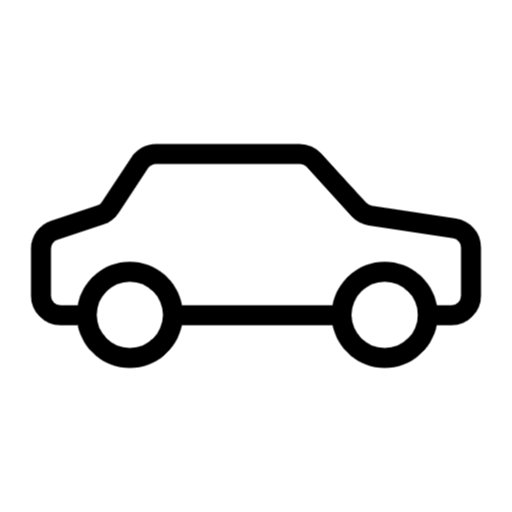
\includegraphics[width=65pt,height=55pt]{Images/car_png.png}};
    \node[car-image] (bike) at (210,122) {
\includegraphics[width=24pt,height=21pt]{Images/bike_png.png}};

    % BLUE CONCENTRATION (c_c)
    \begin{scope}[myblue]
        \draw[dashed-line] (169,64) -- (168,137.4);  % Vertical dashed line
        \draw (162,62.4) -- (177,62.4);  % Top tick mark
        \draw (161,137.4) -- (176,137.4);  % Bottom tick mark
    \end{scope}

    % RED CONCENTRATION (c_c - c_b)
    \begin{scope}[myred]
        \draw[dashed-line] (255,62) -- (255,90.4);  % Vertical dashed line
        \draw (248,62.4) -- (263,62.4);  % Top tick
        \draw (248,93.4) -- (263,93.4);  % Middle tick
    \end{scope}

   % GREEN CONCENTRATION (c_b)
    \begin{scope}[mygreen]
        \draw[dashed-line] (255,135.97) -- (255,108.4);  % Vertical dashed line
        \draw (248,106.4) -- (263,106.4);  % Top tick
        \draw (248,137.4) -- (263,137.4);  % Bottom tick
    \end{scope}
    
    % BLUE ALIGNMENT (c_c => φ_c)
    \begin{scope}[every node/.style={concentration}]  % Apply concentration style
        \node[myblue] (c-label) at (180,79) {$\theta^\mathrm{c}_{a}$};      % x=190, y=90
        \node[myblue] at (200,79) {$\Rightarrow$};        % x=210, y=90
        \node[myblue] (phi-label) at (230,79) {$t_{a}^\mathrm{c}(\phi_a^\mathrm{c})$}; % x=230, y=90
    \end{scope}

    % RED ALIGNMENT (c_c - c_b => φ_c')
    \begin{scope}[every node/.style={concentration}]  % Apply concentration style
        \node[myred] (c-label) at (285,79) {$\downarrow  \theta^\mathrm{c}_{a}$};      % x=275, y=90
        \node[myred] at (318,79) {$\Rightarrow$};            % x=305, y=90
        \node[myred] (phi-label) at (355,79) {$\uparrow t^\mathrm{c}_{a}(\phi_a^\mathrm{c}) $}; % x=325, y=90
    \end{scope}

    % GREEN ALIGNMENT (c_b => φ_b)
    \begin{scope}[every node/.style={concentration}]  % Apply concentration style
        % \node[mygreen] (c-label) at (270,125) {$\theta^\mathrm{b}_{a}$};      % x=270, y=135
        % \node[mygreen] at (290,125) {$\Rightarrow$};        % x=290, y=135
        \node[mygreen] (phi-label) at (280,125) {$\phi_a^\mathrm{b}$}; % x=310, y=135
    \end{scope}

    % DASHED CONNECTION BETWEEN VEHICLES
    \draw[dashed-line] (172,100.36) -- (375,100.36);  % Dashed connection between vehicles
\end{tikzpicture}
\caption{\footnotesize The creation/upgrading of a bike lane is modeled as reducing the capacity of the affected car link, resulting in an increased travel time $\uparrow t^\mathrm{c}_{a}(\phi_a^\mathrm{c})$.}
    \label{bike_impact}
 \end{figure}

\begin{figure}[t]
\vspace{0.2cm}
  \centering
  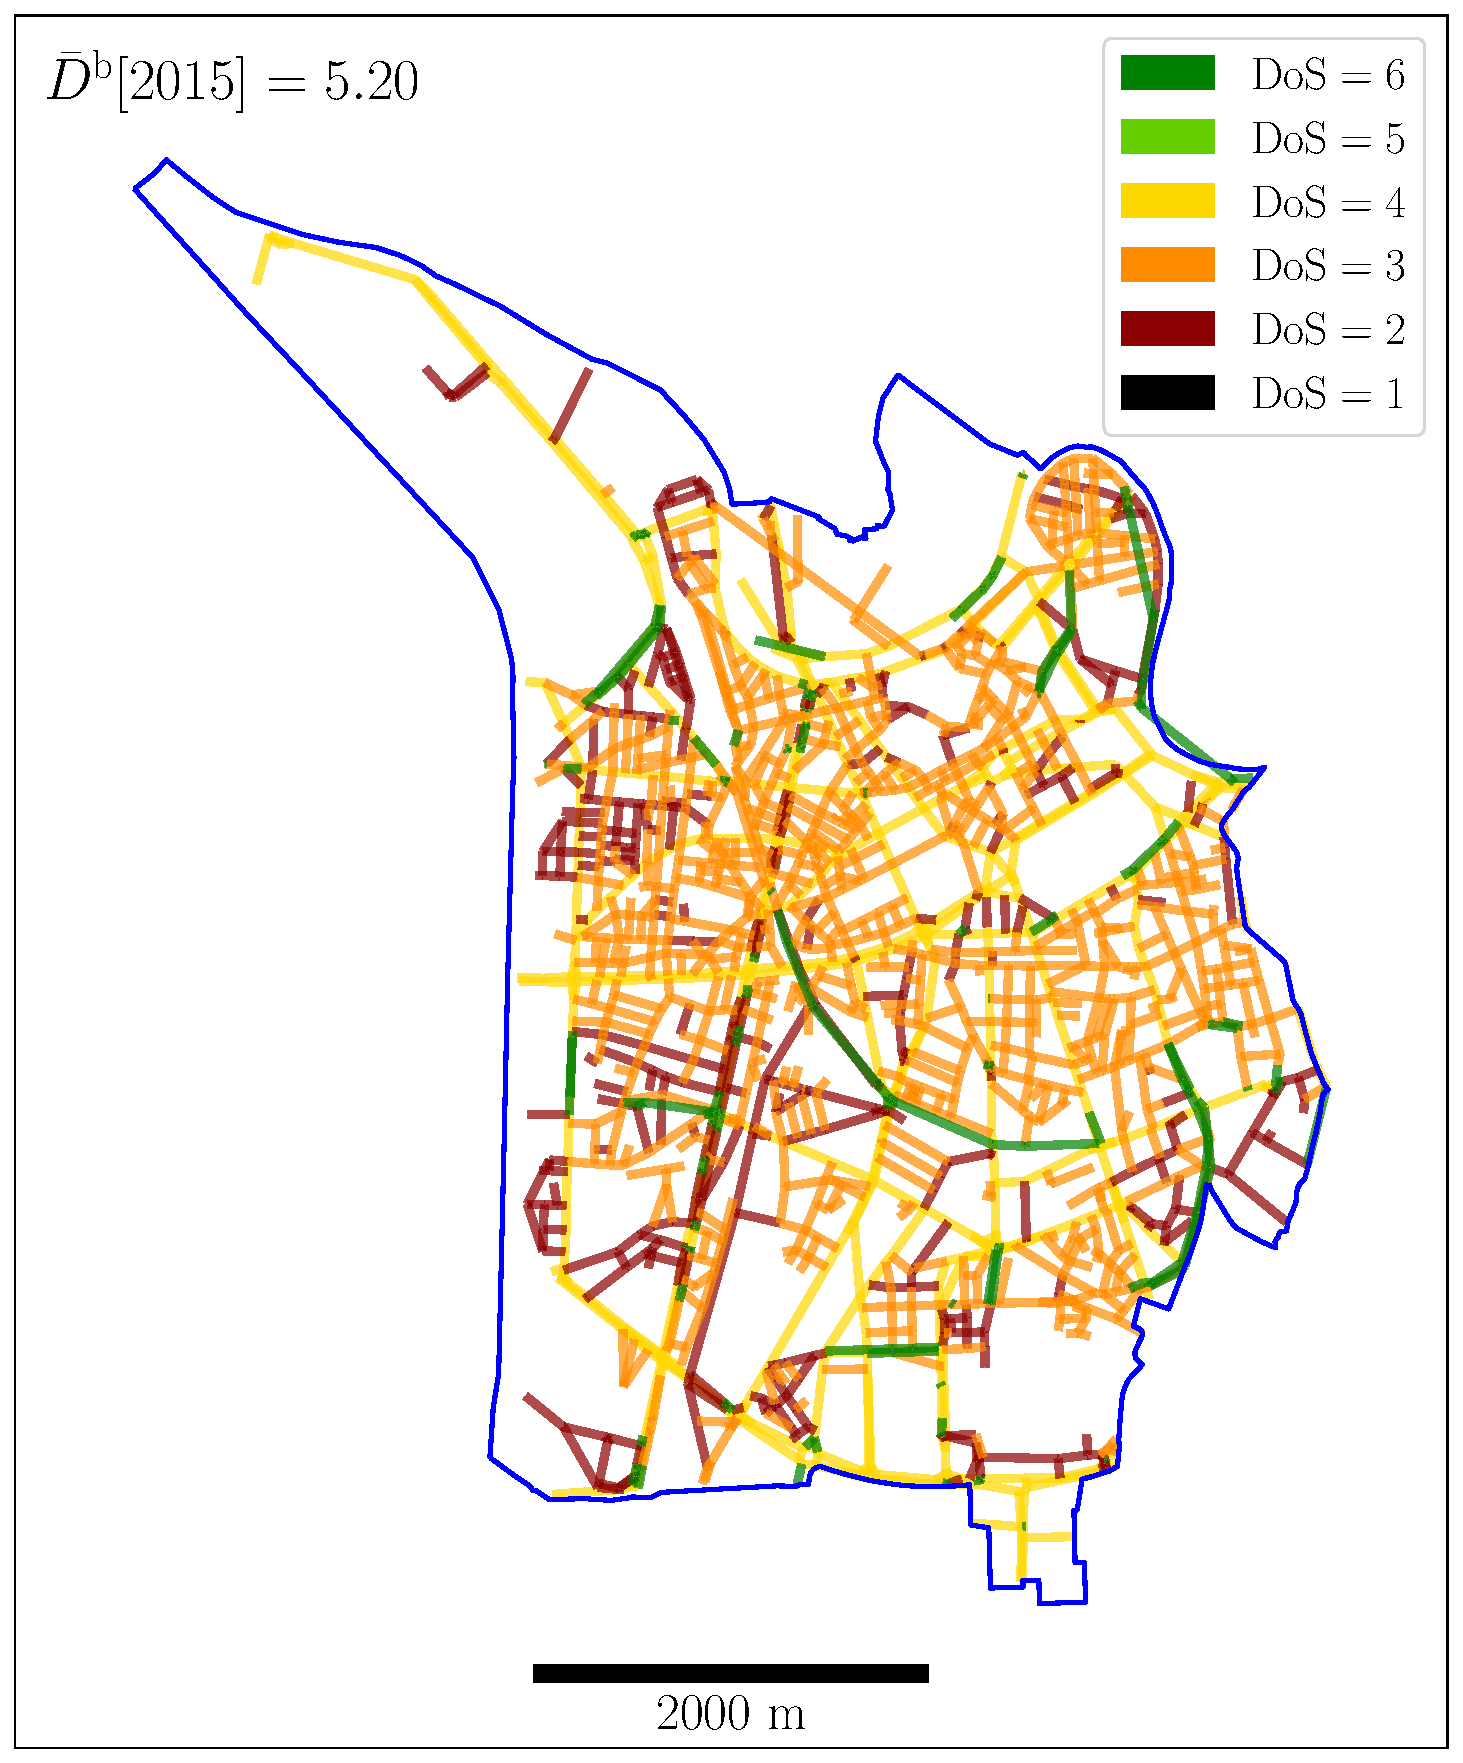
\includegraphics[width=0.48\linewidth]{Images/Grenoble_bikes_network_2015.pdf}
  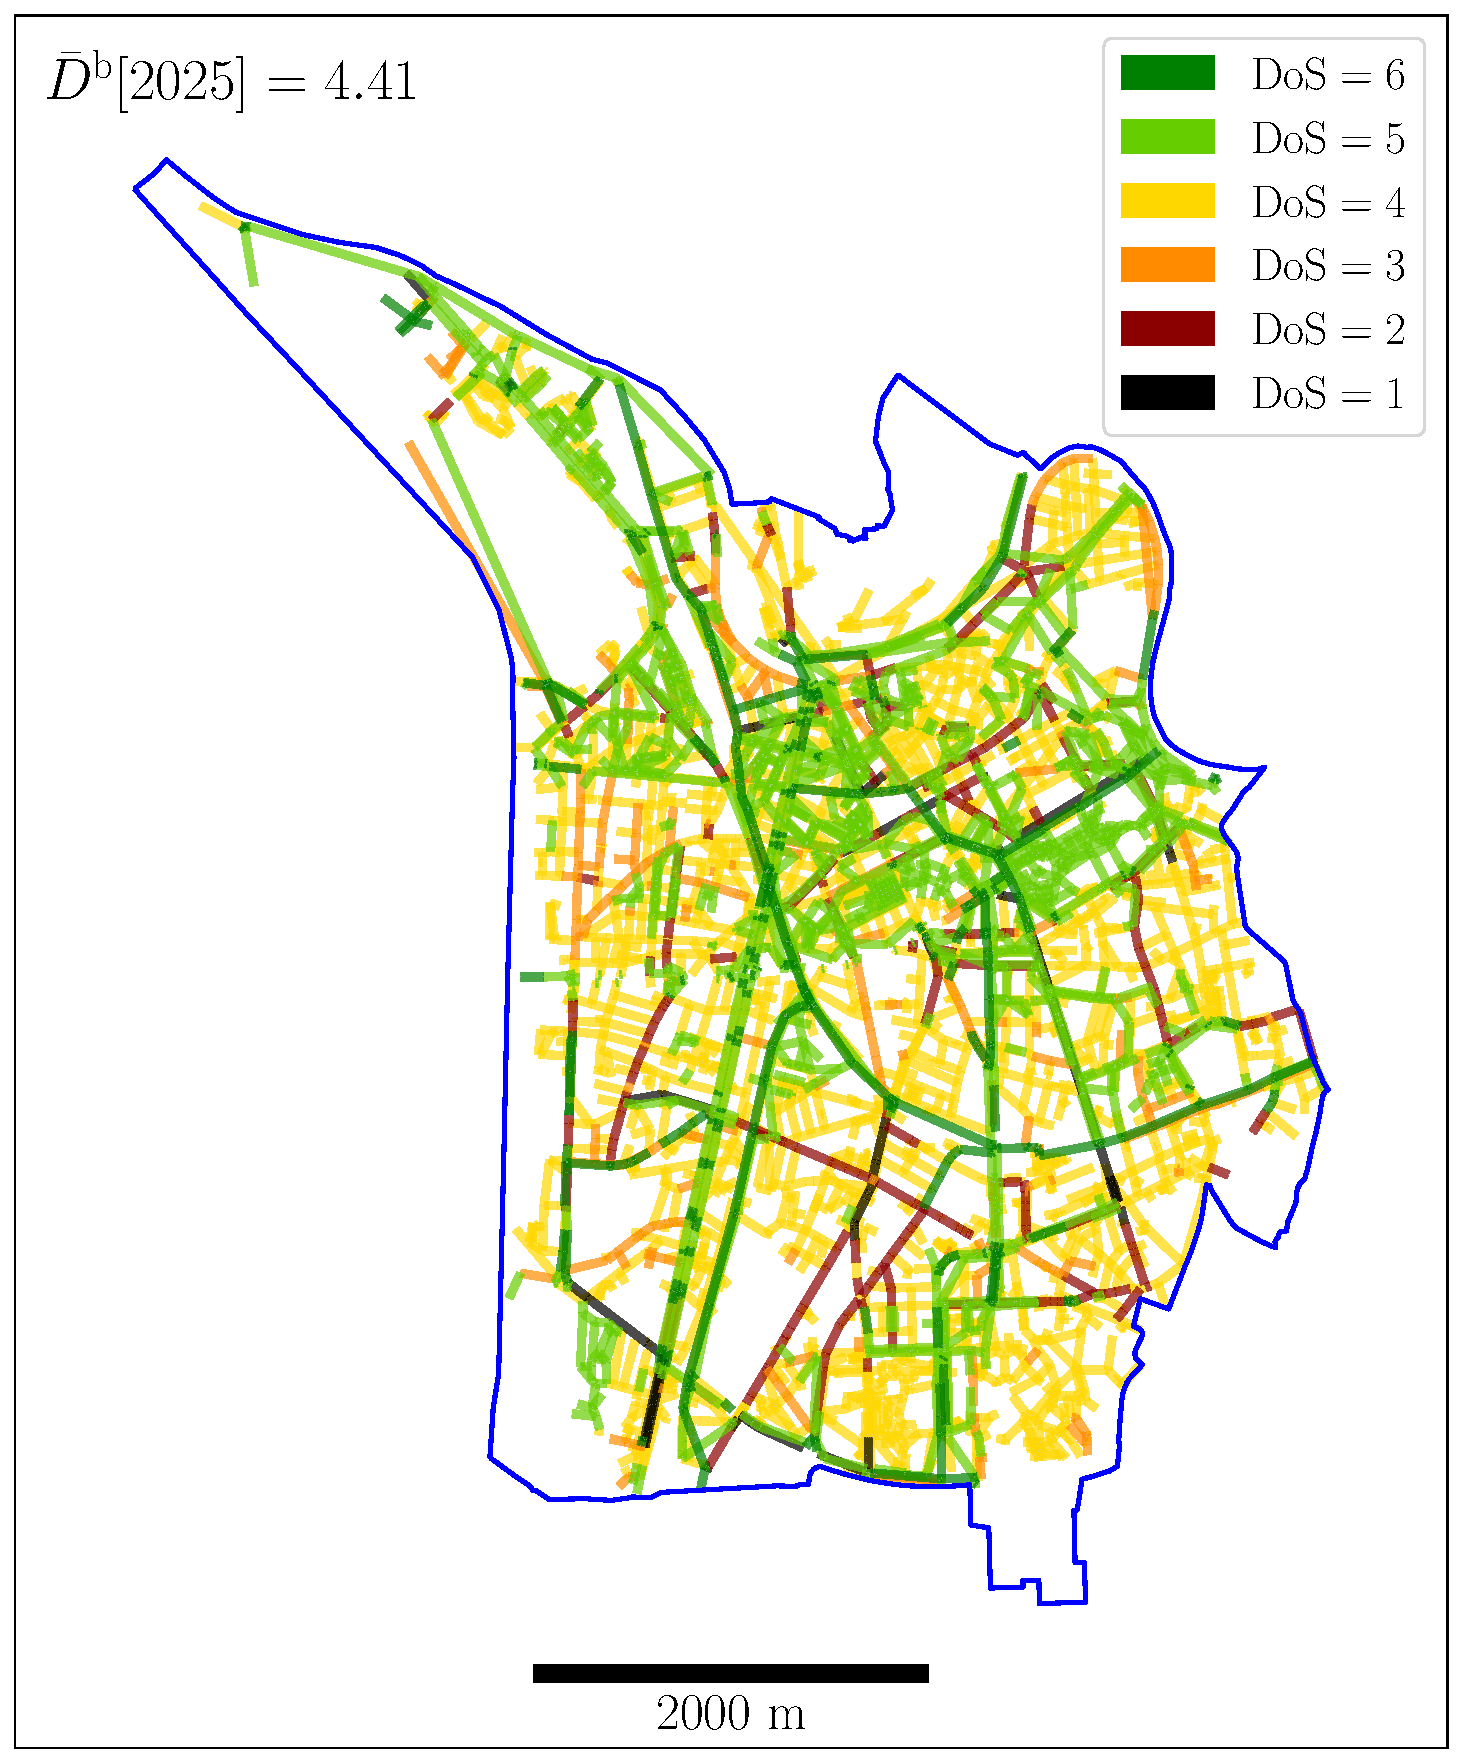
\includegraphics[width=0.48\linewidth]{Images/Grenoble_bikes_network_2025.pdf}
  \caption{\footnotesize Historical cycling network of Grenoble, France. 
  \textit{Left:} year 2015. \textit{Right:} year 2025. The average cycling distance 
2  $\overline{D}^\mathrm{b}[k]$ decreases as the network expands and improves.}
  \label{historical_cycling_network}
\end{figure}

We develop a binary mode choice model linking changes in cycling network quality to variations in bicycle mode share over time, using historical data from the Grenoble metropolitan area.  
The annual cycling networks for 2015--2025 were extracted from OpenStreetMap using the \texttt{OSMnx} Python package \cite{boeing2017}.  
For each year $k \in \{2015, 2016, \ldots, 2025\}$, we compute the average (safety-adjusted) cycling distance as
\begin{equation}
    \overline{D}^\mathrm{b}[k] =
    \frac{1}{|\mathcal{V}_{\mathcal{O}}^\mathrm{b} \times \mathcal{V}_{\mathcal{D}}^\mathrm{b}|}
    \sum_{(u,v) \in \mathcal{V}_{\mathcal{O}}^\mathrm{b} \times \mathcal{V}_{\mathcal{D}}^\mathrm{b}}
    \bar{d}_{(u,v)}^\mathrm{b}[k],
\end{equation}
where $\bar{d}_{(u,v)}^\mathrm{b}[k]$ denotes the cyclist distance between origin $u$ and destination $v$ for the network configuration and traffic conditions of year $k$. Fig.~\ref{historical_cycling_network} illustrates the Grenoble cycling network in 2015 and its projected configuration for 2025.
Fig.~\ref{linear_regression} reports the average cycling distance and the bicycle mode share for the historical network between 2015 and 2025, based on observed values from French National Institute of Statistics and
Economic Studies (INSEE) and other surveys \cite{aller2017, aurg2020, cie2024}, with intermediate years estimated through linear regression.
As shown, there is an inverse relationship between the two variables: the average cycling distance decreases almost monotonically over time, while the bicycle mode share steadily increases, reflecting a progressive shift toward shorter but more frequent cycling trips as infrastructure expands and connectivity improves.
% See Fig.~\ref{historical_cycling_network} for an example of the Grenoble cycling network in 2025 and the current cycling network in 2015. TABLE~\ref{grenoble_historical_table} shows the average cycling distance and the bicycle mode share for the historical Grenoble cycling network between 2015-2025 based on observed values reported in \cite{aller2017, aurg2020, cie2024}, with intermediate years estimated through linear regression.
% \begin{table}[!h]
% \centering
% \begin{tabular}{c|c|c}
% \textbf{Year ($k$)} & \textbf{Average cycling distance $\overline{D}^\mathrm{b}[k]$} & \textbf{Bicycle mode share $P^\mathrm{b}[k]$} \\ \hline
% 2015 & 5.20 & 1.16\% \\
% 2016 & 5.14 & 2.24\% \\
% 2017 & 5.08 & 3.01\% \\
% 2018 & 5.03 & 4.00\% \\
% 2019 & 4.97 & 5.24\% \\
% 2020 & 4.92 & 6.75\% \\
% 2021 & 4.81 & 8.50\% \\
% 2022 & 4.71 & 10.44\% \\
% 2023 & 4.60 & 12.50\% \\
% 2024 & 4.50 & 14.50\% \\
% 2025 & 4.41 & 16.49\% \\
% \end{tabular}
% \caption{Historical safety-adjusted cycling distance and bicycle mode share in Grenoble.}
% \label{grenoble_historical_table}
% \end{table}
% \vspace{0.3em}
% \noindent
\begin{figure}[t]
\vspace{0.2cm}
  \centering
 % \includegraphics[width=0.49\linewidth]{Images/G_original_flow.png}
  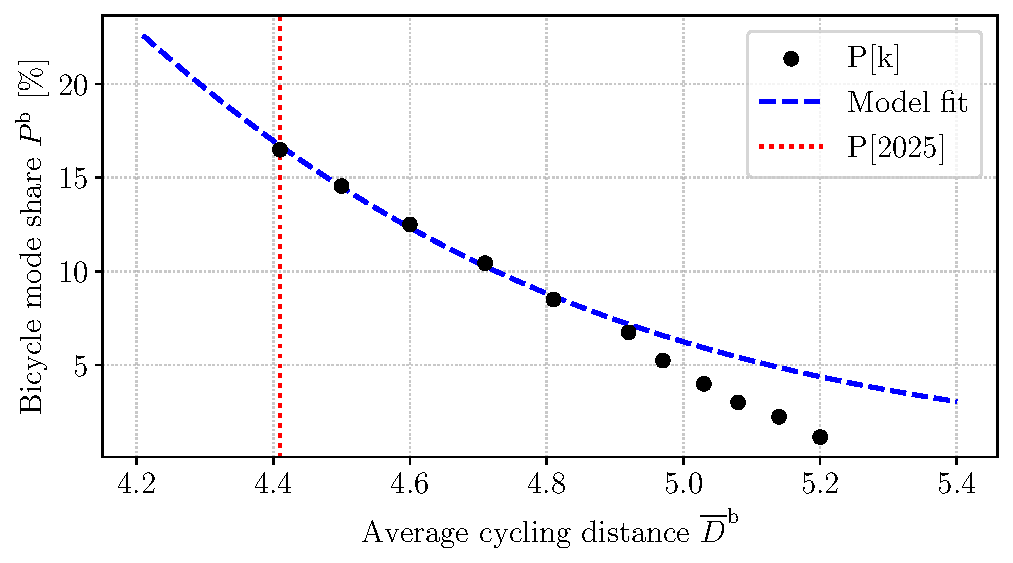
\includegraphics[width=0.9\linewidth]{Images/regression_plot_second.pdf}
  \label{log_a}
  \caption{\footnotesize The logit model plot to predict $P^\mathrm{b}[k]$ using $\bar{D}^\mathrm{b}$.}
  \label{linear_regression}
\end{figure}

We acknowledge that cycling adoption is influenced by a wide range of factors, including social context, municipal initiatives, historical development, and gender dynamics \cite{glachant2024negotiating, parsha2022social}. 
However, in this study we adopt a macroscopic formulation in which infrastructure is the sole explanatory variable of bicycle mode choice. 
This assumption is supported by evidence showing that the quality of cycling facilities strongly affects travel behavior, as cyclists consistently prefer routes separated from motorized traffic, while poor surface conditions tend to discourage cycling \cite{buehler2016bikeway, adam2024agent}. We model the annual probability of choosing cycling, denoted as $ P^\mathrm{b}[k] $, based on the utility associated with the bicycle mode, $ V^\mathrm{b}[k] $. 
This utility is assumed to depend linearly on the average cycling distance $ \overline{D}^\mathrm{b}[k] $
\begin{equation}
\label{eq:bike_utility}
    V^\mathrm{b}[k] = \alpha + \beta\,\overline{D}^\mathrm{b}[k].
\end{equation}
Using a binary logit model, with the car mode as the reference alternative, the probability of choosing the bicycle mode in year $ k $ is expressed as
\begin{equation}
    P^\mathrm{b}[k] = 
    \frac{\exp(V^\mathrm{b}[k])}{\exp(V^\mathrm{b}[k]) + \exp(V^\mathrm{c}[k])}.
\end{equation}
Since only relative utilities influence the choice, we normalize the utility of the car mode to zero ($ V^\mathrm{c} \equiv 0 $) without loss of generality. 
This yields the standard logit formulation 
\begin{equation}
\label{eq:logit_expression}
    P^\mathrm{b}[k] = 
    \frac{\exp(V^\mathrm{b}[k])}{1 + \exp(V^\mathrm{b}[k])}
    = \frac{1}{1 + \exp(-V^\mathrm{b}[k])},
\end{equation}
where $ \alpha $ is an alternative-specific constant capturing unobserved 
factors favoring car use (e.g., travel time, fuel cost, or parking convenience),
and $ \beta < 0 $ represents the sensitivity of the cycling adoption to the
perceived distance or effort. Substituting \eqref{eq:bike_utility} into the logit expression \eqref{eq:logit_expression} yields the predicted 
bicycle mode share
\begin{equation}
    \widehat{P}^\mathrm{b}[k] = 
    \frac{1}{1 + \exp\!\big(-(\alpha + \beta\,\overline{D}^\mathrm{b}[k])\big)}.
\end{equation}
The parameters $ (\alpha, \beta) $ are estimated from the observed annual data pairs
$ \{(\overline{D}^\mathrm{b}[k], P^\mathrm{b}[k])\} $ by minimizing the squared difference between 
observed and predicted bicycle shares:
\begin{equation}
    \min_{\alpha,\beta} 
    \sum_{k}
    \left[
        P^\mathrm{b}[k] - \widehat{P}^\mathrm{b}[k]
    \right]^2.
\end{equation}
To ensure consistency with the current situation, $ \alpha $ is calibrated so that,
for the existing 2025 network, the model reproduces the observed cycling share.
Hence, if no network upgrades are applied 
(\emph{i.e.}, $\boldsymbol{w}^\mathrm{b} $ identical to 2025),
the predicted bicycle probability $ \mathbb{P}^\mathrm{b} $ equals the observed value
$ P^\mathrm{b}_{\mathrm{2025}} $.

For any upgraded configuration $\boldsymbol{w}^\mathrm{b} $, 
the corresponding average cycling distance 
$ \overline{D}^\mathrm{b}(\tilde{\boldsymbol{w}}^\mathrm{b}) $ 
determines the updated mode shares. 
Although $ \overline{D}^\mathrm{b}[k] $ varies over time, it can also be viewed as a function 
of the network configuration $ \boldsymbol{w}^\mathrm{b} $, 
since infrastructure upgrades that increase the DoS, modify travel 
effort and route choices, thus affecting the resulting cycling share.
\begin{align}
    \mathbb{P}^\mathrm{b}(\boldsymbol{w}^\mathrm{b})
        &= \frac{1}{1 + \exp\!\big(-(\alpha + \beta\,\overline{D}^\mathrm{b}(\boldsymbol{w}^\mathrm{b}))\big)},\\[2pt]
    \mathbb{P}^\mathrm{c}(\boldsymbol{w}^\mathrm{b})
        &= 1 - \mathbb{P}^\mathrm{b}(\boldsymbol{w}^\mathrm{b}),
\end{align}
and the total travel demand between each origin–destination pair $ (u,v) $ 
is reallocated as
\begin{align}
\label{eq:mode_shift}
    q_{(u,v)}^\mathrm{b}(\boldsymbol{w}^\mathrm{b})
        &= \mathbb{P}^\mathrm{b}(\boldsymbol{w}^\mathrm{b})\, \cdot Q_{(u,v)},\\[2pt]
    q_{(u,v)}^\mathrm{c}(\boldsymbol{w}^\mathrm{b})
        &= \mathbb{P}^\mathrm{c}(\boldsymbol{w}^\mathrm{b})\, \cdot Q_{(u,v)},
\end{align}
where $ Q_{(u,v)} $ denotes the total travel demand of car drivers and cyclists between origin $ u $ 
and destination $ v $.


\subsubsection{Surrogate-Based Flow Prediction with Feasibility Projection}
\label{subsec:gcn_surrogate}

Computing the UE traffic assignment at each iteration is computationally expensive, particularly when travel demand and lane configurations change frequently due to network upgrades. To mitigate this cost, we employ a graph-based surrogate that predicts near-equilibrium car flows and travel times directly from network-level features, followed by a projection step to ensure feasibility.

Let $\tilde{\boldsymbol{\phi}}^\mathrm{c} = [\tilde{\phi}_a^\mathrm{c}]_{a \in \mathcal{A}^\mathrm{c}}^\top \in \mathbb{R}^{|\mathcal{A}^\mathrm{c}|}$ denote the vector of car flows on all arcs, and let $\tilde{\boldsymbol{q}}^\mathrm{c} = [\tilde{q}_{(u,v)}^\mathrm{c}]_{(u, v) \in \mathcal{V}_{\mathcal{O}}^\mathrm{b}\times \mathcal{V}_{\mathcal{D}}^\mathrm{b}}^\top \in \mathbb{R}^{|\mathcal{V}^\mathrm{c}_{\mathcal{O}} \times \mathcal{V}^\mathrm{c}_{\mathcal{D}}|}$ represent the OD demand vector. The UE flow $\boldsymbol{\phi}^{\mathrm{c}^\star}$ satisfies the flow-conservation constraint
\begin{equation}
    B \tilde{\boldsymbol{\phi}}^{c^{\ast}} = \boldsymbol{d}^\mathrm{c},
\end{equation}
where $B \in \{-1,0,1\}^{|\mathcal{V}^\mathrm{c}| \times |\mathcal{A}^\mathrm{c}|}$ is the node--arc incidence matrix and $\boldsymbol{d}^\mathrm{c} \in \mathbb{R}^{|\mathcal{V}^\mathrm{c}|}$ is the net demand vector (positive at origins, negative at destinations, and zero at intersections and junctions).

We train a Graph Convolutional Network (GCN) surrogate $\mathcal{M}$ on UE traffic assignments obtained under random bike-lane upgrade configurations $\tilde{\boldsymbol{w}}^\mathrm{b}$. 
Each configuration alters the car network capacities and OD demands, generating distinct equilibrium flows and travel times used as ground truth. 
The GCN takes as input the car network topology $\mathcal{A}^\mathrm{c}$, the effective arc capacities $\boldsymbol{\theta}^\mathrm{c} = [\theta_{a}^\mathrm{c}]_{a \in \mathcal{A}^\mathrm{c}}$ from~\eqref{eq:effective_capacity}, and the post-shift OD demand vector 
$\boldsymbol{q}^\mathrm{c} = [q_{(u,v)}^\mathrm{c}]_{(u,v) \in \mathcal{V}_{\mathcal{O}}^\mathrm{c} \times \mathcal{V}_{\mathcal{D}}^\mathrm{c}}^{\top}$ from \eqref{eq:mode_shift}, 
and learns the mapping from network configuration to predict UE traffic flow distribution $\boldsymbol{\phi}^\mathrm{c}$ as follows:
\begin{equation}
    \mathcal{M}:\; (\mathcal{A}^\mathrm{c},\; \boldsymbol{\theta}^\mathrm{c},\; \boldsymbol{q}^\mathrm{c})
    \;\longmapsto\;
    \boldsymbol{\phi}^\mathrm{c}.
\end{equation}

Since these inputs, in particular $\boldsymbol{\theta}^\mathrm{c}$ and potentially $\boldsymbol{q}^\mathrm{c}$ through mode choice, are functions of the upgraded cycling configuration $\boldsymbol{w}^\mathrm{b}$, we write the surrogate compactly as
\begin{equation}
    \mathcal{M}:\; \boldsymbol{w}^\mathrm{b} \;\longmapsto\;
    \boldsymbol{\phi}^\mathrm{c}.
\end{equation}
However, since the GCN does not explicitly enforce flow conservation, $\boldsymbol{\phi}^\mathrm{c}$ may violate $B \boldsymbol{\phi}^\mathrm{c} = \boldsymbol{d}^\mathrm{c}$. We restore feasibility by projecting the surrogate prediction onto the flow-conserving subspace via the quadratic program
\begin{equation}
    \boldsymbol{\phi}^{c^{\star}}
    \;=\;
    \arg\min_{\boldsymbol{\phi}^\mathrm{c} \ge 0}\;
      \big\|\tilde{\boldsymbol{\phi}}^\mathrm{c} - \boldsymbol{\phi}^\mathrm{c}\big\|_2^2
      \quad \text{s.t.}\quad
      B \boldsymbol{\phi}^\mathrm{c} = \boldsymbol{d}^\mathrm{c}.
\end{equation}
The solution $\boldsymbol{\phi}^{c^{\star}}$ represents the Euclidean projection of the GCN-predicted flows onto the feasible subspace, ensuring node-level flow conservation and nonnegativity. 
The corresponding car total system travel time associated with $\boldsymbol{\phi}^{c^{\star}}$ is  denoted as $\mathcal{T}^\mathrm{c}(\boldsymbol{w}^\mathrm{b})$. 
Finally, the surrogate-based total system travel time combines the computed bicycle component with the GCN-predicted car component
\begin{equation}
\label{total_system_travel}
    \mathcal{T}_{\mathrm{tot}}(\boldsymbol{w}^\mathrm{b})
    \;=\;
    \mathcal{T}_\mathrm{b}(\boldsymbol{w}^\mathrm{b})
    \;+\;
    \mathcal{T}_\mathrm{c}(\boldsymbol{w}^\mathrm{b}).
\end{equation}
This GCN--projection framework provides fast and consistent approximations of network performance, enabling efficient optimization of multi-modal configurations while substantially reducing computational cost. A detailed assessment of the model’s predictive accuracy and reliability is presented in the Results section.


\subsection{Optimization Problem (Utilitarian Perspective)}

We now introduce the utilitarian formulation of the trade-off problem for upgrading cycling infrastructure. 
Under a utilitarian perspective, the planner seeks to improve the overall performance of the transport system by minimizing aggregate costs across users. 
Given a fixed budget $B$, the planner selects a subset of road segments to upgrade in order to enhance their degree of separation. 
The objective balances two competing goals: (i) minimizing cyclists’ average exposure to motor traffic, and (ii) limiting the aggregate increase in total travel times due to car capacity reallocation. 
This formulation therefore aims to reduce the overall system cost by jointly accounting for traffic exposure and travel-time inefficiency.

Let the decision variables
\begin{equation}
    \boldsymbol{w}^\mathrm{b} = \big[w_{a}^\mathrm{b}\big]_{a \in \mathcal{A}^\mathrm{b}}^\top
\end{equation}
denote the vector of upgraded DoS values for all bicycle arcs, with the feasible set
\begin{equation}
    \Omega = \Big\{\boldsymbol{w}^\mathrm{b} \in \{1,\dots,6\}^{|\mathcal{A}^\mathrm{b}|} :
    \tilde{w}_a^\mathrm{b} \leq w_a^\mathrm{b} \leq 6, \;\forall a \in \mathcal{A}^\mathrm{b} \Big\}.
\end{equation}

% Table~\ref{tab:variables_utilitarian} summarizes the main quantities used in the optimization model.

% \begin{table}[!h]
% \centering
% \caption{Notation used in the utilitarian optimization formulation.}
% \label{tab:variables_utilitarian}
% \begin{tabular}{l|c|c|c}
% \textbf{Symbol} & \textbf{Description} & \textbf{Domain} & \textbf{Unit} \\ \hline
% $\phi_a^\mathrm{b}(\boldsymbol{w}^\mathrm{b})$ & Bicycle flow on arc $a$ & $\mathbb{R}_{\geq 0}$ & bike/day \\
% $d_a^\mathrm{b}$ & Length of bike arc $a$ & $\mathbb{R}_{>0}$ & m \\
% $\bar{d}_a^\mathrm{b}(\boldsymbol{w}^\mathrm{b})$ & Cyclist distance on arc $a$ & $\mathbb{R}_{>0}$ & m \\
% $\mathcal{E}_a(\boldsymbol{w}^\mathrm{b})$ & Cyclist exposure on arc $a$ & $\mathbb{R}_{\geq 0}$ & –  \\
% $\pi(\tilde{w}_a^\mathrm{b}, w_a^\mathrm{b})$ & Upgrade cost of arc $a$ & $\mathbb{R}_{\geq 0}$ & \text{€} \\
% $\theta_a^\mathrm{c}(\boldsymbol{w}^\mathrm{b})$ & Updated car lane capacity on arc $a$ & $\mathbb{R}_{\geq 0}$ & veh/day \\
% $\mathcal{T}_{\mathrm{tot}}(\boldsymbol{w}^\mathrm{b})$ & Predicted total travel time & $\mathbb{R}_{\geq 0}$ & $\frac{\mathrm{travelers}\cdot \mathrm{hr}}{\mathrm{day}}$ \\ \hline
% \end{tabular}
% \end{table}

We formulate the problem as a bi-level optimization, where the upper level determines infrastructure upgrades, and the lower level models the resulting cyclist route choices.

At the \textit{upper level} ($\mathbb{U}$), the planner selects upgrades $\boldsymbol{w}^\mathrm{b}~\in~\Omega$ subject to the budget $B$, minimizing total cyclist exposure and total travel time while controlling the impact on the average car total travel times. The formulation naturally prioritizes the improvement of longer links with both high cyclist and vehicle volumes, since these contribute most to total exposure and travel cost.

At the \textit{lower level} ($\mathbb{L}$), given a specific upgraded configuration $\boldsymbol{w}^\mathrm{b}$, cyclist flows are assigned to origin–destination pairs using an all-or-nothing (AON) shortest-path assignment based on the effective cyclist distance defined in Section~\ref{cyclist_exposure}. This ensures that the induced flow distribution reflects perceived safety across the network.
\begin{problem}[\textbf{Utilitarian Trade-Off Network Upgrade}]
\label{trade_off_problem_util}
\begin{align}
\mathbb{U}: \quad  \, &  \boldsymbol{w}^{\mathrm{b}^\star} 
= \arg\min_{\boldsymbol{w}^\mathrm{b} \in \Omega} 
\;\; \gamma \cdot 
\underbrace{\sum_{a \in \mathcal{A}^\mathrm{b}} \phi_{a}^{\mathrm{b}^{\star}}(\boldsymbol{w}^\mathrm{b}) \cdot f_a^\mathrm{b}(\boldsymbol{w}^\mathrm{b}) \cdot d_a^\mathrm{b} }_{\text{Cyclist exposure } J_{\mathcal{E}}(\boldsymbol{w}^\mathrm{b})}
\nonumber \\
& \hspace{2.5cm} + (1-\gamma)\cdot 
\underbrace{\mathcal{T}_{\mathrm{tot}}(\boldsymbol{w}^\mathrm{b})}_{\text{Predicted total travel time}}
\label{eq:upper_util} \\
\text{s.t. } &\quad \sum_{a \in \mathcal{A}^\mathrm{b}} d_a^\mathrm{b} \cdot \pi(\tilde{w}_a^\mathrm{b},w_a^\mathrm{b}) \;\leq\; B, \label{eq:budget_util} \\
&\quad \theta_a^\mathrm{c}(\boldsymbol{w}^\mathrm{b}) 
    = \tilde{\theta}_a^\mathrm{c}
\left(1-\frac{z_a}{n_a^\mathrm{c}}\right), \label{eq:effective_capacity_ut}
\end{align}
where the lower-level bicycle flow assignment is
\begin{align}
\mathbb{L}: \quad \, & 
 \boldsymbol{\phi}^{\mathrm{b}^\star}(\boldsymbol{w}^\mathrm{b}) 
= \arg\min_{\boldsymbol{\phi}^\mathrm{b} \in \mathbb{R}_{\geq 0}^{|\mathcal{A}^\mathrm{b}|}}
\sum_{a \in \mathcal{A}^\mathrm{b}} \bar{d}_a^\mathrm{b}(\boldsymbol{w}^\mathrm{b}) \cdot \phi_a^\mathrm{b}
\label{eq:lower_util} \\
\text{s.t. } &\quad \phi_a^\mathrm{b} = \sum_{(u,v) \in \mathcal{V}^\mathrm{b}_\mathcal{O} \times \mathcal{V}^\mathrm{b}_\mathcal{D}}
q_{(u,v)}^\mathrm{b}(\boldsymbol{w}^\mathrm{b}) \cdot \mathbb{I}_{a \in p_{(u,v)}^\mathrm{b}}, \quad \forall a \in \mathcal{A}^\mathrm{b}. \nonumber
\end{align}
\end{problem}
The two objective terms are normalized by their values in the original network configuration, so that cyclist exposure and total travel time become dimensionless and comparable. The parameter $\gamma \in [0,1]$ controls the trade-off between the two terms: Larger values of $\gamma$ give more importance to reducing cyclist exposure, whereas smaller values give more importance to limiting total travel-time impacts. The budget constraint~\eqref{eq:budget_util} ensures feasibility of the selected infrastructure upgrades, while the capacity relation~\eqref{eq:effective_capacity_ut} captures the reduction in car capacity when high-quality separated bicycle infrastructure (DoS $\geq 5$) is introduced. The lower-level problem~\eqref{eq:lower_util} assigns bicycle flows through an all-or-nothing shortest-path model under the updated generalized cyclist distances and the new bicycle demand resulting from modal shifts. These flows $\boldsymbol{\phi}^{\mathrm{b}\star}(\boldsymbol{w}^\mathrm{b})$ then enter the upper-level objective, ensuring consistency between infrastructure upgrades, route choices, flows, and exposure.


The bi-level optimization in Problem~2 is $\text{NP}\text{-hard}$, as it generalizes the 0-1 knapsack problem where each arc upgrade represents an item with cost $\pi(\tilde{w}_a^\mathrm{b},w_a^\mathrm{b})$ and  benefits both  cyclist exposure and traffic flow. The complexity arises from the combinatorial upgrade choices under budget $B$, and the evaluation of cyclist exposure and non-linear car flow effects from changes in $\theta_a^\mathrm{c}$.

% \subsection{Optimization Problem (Sufficientarian Perspective)}
% \label{section_safety_metric}
% Now, we incorporate a sufficientarian perspective into Problem~1 by ensuring that as many individuals as possible achieve a minimum level of safety on paths throughout the network. Using the a similar definition of \eqref{arc_exposure}, for a path $p_{(u,v)}^\mathrm{b}$ between OD pair $(u,v)$, we define the safety score as
% \begin{equation}
%     S_{p_{(u,v)}^\mathrm{b}} = \frac{1}{\sum_{a \in p_{(u,v)}^\mathrm{b}} f_a^\mathrm{b} \cdot d_a^\mathrm{b}   + \epsilon},
% \end{equation}
% where $\phi_{a}^\mathrm{b}$ is the cyclist flow on arc $a$, $f_a^\mathrm{b}$ is the traffic-related risk factor, $d_a^\mathrm{b}$ is its length, and $\epsilon>0$ avoids division by zero and limits the maximum safety score. This score reflects the inverse relationship between cyclist exposure and perceived safety, consistent with established findings in route choice modeling \cite{casello2014modeling}, where cyclists prefer routes with lower traffic volumes. Although this formulation is a simplification, it serves as a continuous proxy for perceived safety when only exposure data is available. 
% \subsection{Optimization Problem (Sufficientarian Perspective)}
% \label{section_safety_metric}

% We now adopt a sufficientarian perspective by targeting a minimum level of perceived cycling safety for as many trips as possible. Empirical evidence shows that perceived safety is strongly shaped by motor-traffic conditions (notably traffic volume and speed) and by the presence and quality of protective infrastructure, and that these perceptions can be reasonably approximated by objective, exposure-based scores when detailed conflict or crash data are not
% available \cite{amiour2022objective,fuest2023bet,useche2019healthy}. Following this rationale, we define an exposure-based path sufficiency score that decreases with the average traffic exposure experienced along the selected cycling path. We use average exposure, rather than cumulative exposure, because the aim of the sufficientarian formulation is not to penalize long trips only for being long, but to identify paths whose protection level is inadequate relative to their length. Total exposure is instead accounted for separately in the utilitarian objective. Therefore, the score below should be interpreted as a normalized indicator of exposure-based path protection, rather than as a direct measure of crash risk or observed safety.


% For a bicycle OD pair $(u,v)$ with selected path $p_{(u,v)}^\mathrm{b}$, we define
% \begin{equation}
% \label{eq:path_safety_score}
% S_{p_{(u,v)}^\mathrm{b}}
% \;=\;
% \frac{1}{
% \displaystyle
% \frac{\sum_{a \in p_{(u,v)}^\mathrm{b}} f_a^\mathrm{b}\, d_a^\mathrm{b}}
% {\sum_{a \in p_{(u,v)}^\mathrm{b}} d_a^\mathrm{b}}
% \;+\;1},
% \end{equation}
% where $f_a^\mathrm{b}$ is the traffic-related exposure factor on arc $a$, and $d_a^\mathrm{b}$ is its length. The term $1$ keeps the score bounded between $0$ and $1$. Higher values indicate paths with lower average exposure to motor traffic, while lower values identify paths with insufficient exposure-based protection \cite{amiour2022objective,fuest2023bet,useche2019healthy}.


% To determine what constitutes a sufficient level of safety, we adopt a relative threshold approach. Let the global average safety across all regions be
% \begin{equation}
%     S_{\mathcal{G}}^\mathrm{b} = \frac{1}{|\mathcal{V}^\mathrm{b}|^2} \sum_{(u,v) \in \mathcal{V}^\mathrm{b} \times \mathcal{V}^\mathrm{b}} S_{p_{(u,v)}^\mathrm{b}}.
% \end{equation}
% We then define a relative path-exposure-based path-protection threshold $s_{\text{thr}}$ as a proportion of the average safety level $s_{\mathcal{G}}^\mathrm{b}$, using a parameter $\lambda$ that takes values from the set $\{10\%, 20\%, 30\%, 40\%, 50\%\}$.
% \begin{equation}
%     S_{\text{thr}} = \lambda S_{\mathcal{G}}^\mathrm{b}.
% \end{equation}

% This method follows the standard practice proposed by Martens in the context of transport justice~\cite{martens2017transport, martens2022equity}, where sufficiency thresholds are defined as a proportion of an average (or median) accessibility level. Cycle trips whose safety scores fall below this threshold ($S_{p_{(u,v)}^\mathrm{b}} \leq S_{\text{thr}}$) are considered insufficiently protected.
% To quantify this shortfall, and following a similar approach to~\cite{salazar2024accessibility}, we adopt a linear form of the Foster–Greer–Thorbecke (FGT) index, originally developed for poverty measurement~\cite{martens2016transport}. In the FGT framework, deprivation is measured as the normalized gap between an individual’s income and a predefined poverty line; analogously, here we measure the exposure-based path insufficiency of each path as the normalized deficit of its safety score relative to the threshold
% \begin{equation}
%     \mathcal{I}_{p_{(u,v)}^\mathrm{b}} = \max \left\{ 0, \; \frac{S_{\text{thr}} - S_{p_{(u,v)}^\mathrm{b}}}{S_{\text{thr}}} \right\}.
% \end{equation}
% This formulation provides a continuous and interpretable measure of how far below the sufficiency threshold a given cycling path falls, enabling aggregate indicators of safety equity across the network.
% Dividing the network into regions $\mathcal{R} = \{1, \dots, R\}$, where $\mathcal{V}^\mathrm{b}_{r} \subseteq \mathcal{V}^\mathrm{b}$ represents nodes in region $r$, allows for regional analysis, then, the regional exposure-based path insufficiency is computed as the demand-weighted average exposure-based path insufficiency for each OD pair within the region
% \begin{equation}
%     \mathcal{I}_r(\boldsymbol{w}^\mathrm{b}) =
%     \frac{\sum_{u \in \mathcal{V}_r^\mathrm{b}} \mathcal{I}_{p_{(u,v)}^\mathrm{b}} \cdot q_{(u,v)}^\mathrm{b}}{\sum_{u \in \mathcal{V}_r^\mathrm{b}} q_{(u,v)}^\mathrm{b}}, 
%     \quad \forall v \in \mathcal{V}^\mathrm{b},
% \end{equation}
% where $q_{(u,v)}^\mathrm{b}$ is the demand for OD pair $(u,v)$. The total population-weighted exposure-based path insufficiency across the network is given by
% \begin{equation}
%     J_{\mathrm{SI}}(\boldsymbol{w}^\mathrm{b}) = 
%     \frac{\sum_{r \in \mathcal{R}} n_r^\mathrm{b} \, \mathcal{I}_r(\boldsymbol{w}^\mathrm{b})}{\sum_{r \in \mathcal{R}} n_r^\mathrm{b}}.
% \end{equation}
% where $n_{r}$ represents the number of cyclists in region $r$. 

% To formulate the sufficientarian perspective in terms of temporal accessibility for both cars and bicycles, we first introduce a path travel time threshold denoted by $T_{\mathrm{thr}}$ (e.g., $T_{\mathrm{thr}} = 20~\text{min} = 1200$\,s, as used in \cite{salazar2024accessibility}). 
% For bicycles, given any trip $(u,v)$ and its corresponding chosen path $p_{(u,v)}$, and using the previously defined path travel time $T_{p_{(u,v)}}^\mathrm{b}$ in \eqref{bike_travel_time}, the trip insufficiency is defined as
% \begin{equation}
% \label{eq:time_insufficiency}
% \mathcal{I}_{p_{(u,v)}}^\mathrm{b} 
% \;=\; \max\!\left\{0,\; 
% \frac{T_{p_{(u,v)}}^\mathrm{b} - T_{\mathrm{thr}}}{T_{\mathrm{thr}}} 
% \right\}.
% \end{equation}
% This quantity measures how much longer a bicycle trip takes compared to the acceptable travel-time threshold $T_{\mathrm{thr}}$. 
% A trip between $u$ and $v$ is considered accessible if its travel time does not exceed the threshold ($T_{p_{(u,v)}}^\mathrm{b} \leq T_{\mathrm{thr}}$), and unaccessible otherwise. 
% Hence, $\mathcal{I}_{p_{(u,v)}}^\mathrm{b}$ represents the relative excess of travel time beyond this limit. 
% To capture cyclists trip insufficiency at a regional level, we consider the demand-weighted average of trip-level insufficiency for all trips originating in region $r$:
% \begin{equation}
% \label{eq:region_insuff_time}
% \mathcal{I}^\mathrm{b}_r(\boldsymbol{w}^\mathrm{b})
% \;=\;
% \frac{\sum_{(u,v):\,u\in\mathcal{V}_r^\mathrm{b}} 
% \mathcal{I}_{p_{(u,v)}}^\mathrm{b} \cdot q^\mathrm{b}_{(u,v)}}
% {\sum_{(u,v):\,u\in\mathcal{V}_r^\mathrm{b}} q^\mathrm{b}_{(u,v)}}.
% \end{equation}
% This formulation ensures that regions with higher cycling demand exert a proportionally greater influence on the overall insufficiency measure. 
% To evaluate cyclist trip insufficiency at the network level, we define the cyclist-weighted network time trip insufficiency, which aggregates regional accessibilities unfairness according to the number of cyclists $n_r^\mathrm{b}$ in each region:
% \begin{equation}
% \label{eq:network_insuff_time}
% J_{\mathrm{TI}}^\mathrm{b}(\boldsymbol{w}^\mathrm{b})
% \;=\;
% \frac{\sum_{r\in\mathcal{R}} n_r^\mathrm{b} \cdot \mathcal{I}_r^\mathrm{b}(\boldsymbol{w}^\mathrm{b})}
% {\sum_{r\in\mathcal{R}} n_r^\mathrm{b}}.
% \end{equation}
% This indicator provides a system-level measure of time trip insufficiency, reflecting the share of the cycling population whose trips exceed acceptable travel-time limits. Analogously, we define drivers-weighted network time trip insufficiency $J_{\mathrm{TI}}^\mathrm{c}(\boldsymbol{w}^\mathrm{b})$ for cars. 

% Finally, we define the sufficientarian bi-level optimization problem, where $\mathbb{U}_{\text{thr}}$ ensures that as many cyclists as possible reach a path-exposure-based path-protection threshold and as many cyclist and drivers as possible meet the minimum path travel time threshold. As in the utilitarian formulation, the lower level $\mathbb{L}$ 
% determines the resulting cyclist flow distribution under the upgraded network.

%%%%%%%%%%%%%%%%%%%%%%%%%%%%%%%%%%%%%%%%%
\subsection{Optimization Problem (Sufficientarian Perspective)}
\label{section_safety_metric}

We now adopt a sufficientarian perspective by targeting a minimum acceptable level of exposure-based path protection for as many cycling trips as possible. Empirical evidence shows that perceived cycling safety is strongly shaped by motor-traffic conditions, notably traffic volume and speed, and by the presence and quality of protective infrastructure. When detailed conflict or crash data are not available, these perceptions can be approximated through objective, exposure-based indicators \cite{amiour2022objective,fuest2023bet,useche2019healthy}. Following this rationale, we define an exposure-based path sufficiency score that decreases with the average traffic exposure experienced along the selected cycling path. We use average exposure, rather than cumulative exposure, because the sufficientarian formulation aims to identify paths whose protection level is inadequate relative to their length, rather than penalizing long trips only because they are long. Total cyclist exposure is instead accounted for separately in the utilitarian objective. Therefore, the score below should be interpreted as a normalized indicator of exposure-based path protection, rather than as a direct measure of crash risk or observed safety.

For a bicycle OD pair $(u,v)$ with selected path $p_{(u,v)}^\mathrm{b}$, we define
\begin{equation}
\label{eq:path_safety_score}
S_{p_{(u,v)}^\mathrm{b}}
\;=\;
\frac{1}{
\displaystyle
\frac{\sum_{a \in p_{(u,v)}^\mathrm{b}} f_a^\mathrm{b}\, d_a^\mathrm{b}}
{\sum_{a \in p_{(u,v)}^\mathrm{b}} d_a^\mathrm{b}}
\;+\;1},
\end{equation}
where $f_a^\mathrm{b}$ is the traffic-related exposure factor on arc $a$, and $d_a^\mathrm{b}$ is its length. The term $1$ keeps the score bounded between $0$ and $1$. Higher values indicate paths with lower average exposure to motor traffic, while lower values identify paths with weaker exposure-based protection \cite{amiour2022objective,fuest2023bet,useche2019healthy}.

To determine what constitutes a sufficient level of exposure-based path protection, we adopt a relative threshold approach. Let the global average path sufficiency score be
\begin{equation}
    S_{\mathcal{G}}^\mathrm{b}
    =
    \frac{1}{|\mathcal{V}^\mathrm{b}|^2}
    \sum_{(u,v) \in \mathcal{V}^\mathrm{b} \times \mathcal{V}^\mathrm{b}}
    S_{p_{(u,v)}^\mathrm{b}}.
\end{equation}
We then define a relative path-sufficiency threshold $S_{\text{thr}}$ as a proportion of the average score $S_{\mathcal{G}}^\mathrm{b}$, using a parameter $\lambda$ that takes values from the set $\{10\%, 20\%, 30\%, 40\%, 50\%\}$:
\begin{equation}
    S_{\text{thr}} = \lambda S_{\mathcal{G}}^\mathrm{b}.
\end{equation}

This method follows the sufficientarian logic used in transport justice~\cite{martens2017transport,martens2022equity}, where sufficiency thresholds are defined as a proportion of an average or reference value. Cycling paths whose scores fall below this threshold, i.e., $S_{p_{(u,v)}^\mathrm{b}} \leq S_{\text{thr}}$, are considered insufficiently protected in exposure-based terms.

To quantify this shortfall, and following a similar approach to~\cite{salazar2024accessibility}, we adopt a linear form of the Foster--Greer--Thorbecke (FGT) index, originally developed for poverty measurement, which is well suited to capture transport injustice~\cite{martens2017transport, pereira2017distributive}. In the FGT framework, deprivation is measured as the normalized gap between an observed value and a predefined threshold. Analogously, here we measure the exposure-based path insufficiency as the normalized deficit of the path score relative to the sufficiency threshold
\begin{equation}
    \mathcal{I}_{p_{(u,v)}^\mathrm{b}}
    =
    \max \left\{
    0,\;
    \frac{S_{\text{thr}} - S_{p_{(u,v)}^\mathrm{b}}}{S_{\text{thr}}}
    \right\}.
\end{equation}
This quantity is zero when the selected path meets or exceeds the threshold and increases continuously as the path-sufficiency score falls further below it. It should therefore be interpreted as a normalized exposure-based protection deficit, rather than as a direct measure of crash risk, welfare loss, or accessibility deprivation. This deficit measure enables aggregation across trips and regions to characterize exposure-based path insufficiency at the network level.


Dividing the network into regions $\mathcal{R} = \{1,\dots,R\}$, where
$\mathcal{V}_r^\mathrm{b} \subseteq \mathcal{V}^\mathrm{b}$ represents the set of
bicycle nodes in region $r$, allows the exposure-based path insufficiency to be
evaluated spatially. We use a demand-weighted average over all bicycle trips
originating in region $r$,
\begin{equation}
    \mathcal{I}_r(\boldsymbol{w}^\mathrm{b})
    =
    \frac{
    \sum_{(u,v):\,u\in\mathcal{V}_r^\mathrm{b}}
    \mathcal{I}_{p_{(u,v)}^\mathrm{b}} \cdot q_{(u,v)}^\mathrm{b}
    }{
    \sum_{(u,v):\,u\in\mathcal{V}_r^\mathrm{b}}
    q_{(u,v)}^\mathrm{b}
    }.
\end{equation}
Here, $\mathcal{I}_{p_{(u,v)}^\mathrm{b}}$ denotes the exposure-based path
insufficiency of the selected cycling path, and $q_{(u,v)}^\mathrm{b}$ is the
bicycle demand for OD pair $(u,v)$. The total population-weighted exposure-based path insufficiency across the network is given by
\begin{equation}
    J_{\mathrm{SI}}(\boldsymbol{w}^\mathrm{b})
    =
    \frac{
    \sum_{r \in \mathcal{R}}
    n_r^\mathrm{b} \, \mathcal{I}_r(\boldsymbol{w}^\mathrm{b})
    }{
    \sum_{r \in \mathcal{R}} n_r^\mathrm{b}
    },
\end{equation}
where $n_r^\mathrm{b}$ represents the number of cyclists in region $r$.

To formulate the sufficientarian perspective in terms of trip travel time for both cars and bicycles, we first introduce a path travel-time threshold denoted by $T_{\mathrm{thr}}$; for example, $T_{\mathrm{thr}} = 20~\text{min} = 1200$\,s, as used in \cite{salazar2024accessibility}. For bicycles, given any trip $(u,v)$ and its corresponding chosen path $p_{(u,v)}^\mathrm{b}$, and using the previously defined path travel time $T_{p_{(u,v)}}^\mathrm{b}$ in \eqref{bike_travel_time}, the bicycle trip insufficiency is defined as
\begin{equation}
\label{eq:time_insufficiency}
\mathcal{I}_{p_{(u,v)}}^\mathrm{b}
\;=\;
\max\!\left\{
0,\;
\frac{T_{p_{(u,v)}}^\mathrm{b} - T_{\mathrm{thr}}}{T_{\mathrm{thr}}}
\right\}.
\end{equation}
This quantity measures the relative excess travel time above the acceptable threshold $T_{\mathrm{thr}}$. A trip between $u$ and $v$ is considered trip-sufficient if its travel time does not exceed the threshold, i.e., $T_{p_{(u,v)}}^\mathrm{b} \leq T_{\mathrm{thr}}$, and trip-insufficient otherwise. Hence, $\mathcal{I}_{p_{(u,v)}}^\mathrm{b}$ represents the relative excess travel time beyond this limit.

We use the same demand-weighted regional aggregation for trip-time
insufficiency, but now the trip-level quantity is
$\mathcal{I}_{p_{(u,v)}}^\mathrm{b}$, which measures excess bicycle travel time
relative to $T_{\mathrm{thr}}$. Thus, cyclists' regional trip insufficiency is
defined as
\begin{equation}
\label{eq:region_insuff_time}
\mathcal{I}^\mathrm{b}_r(\boldsymbol{w}^\mathrm{b})
\;=\;
\frac{
\sum_{(u,v):\,u\in\mathcal{V}_r^\mathrm{b}}
\mathcal{I}_{p_{(u,v)}}^\mathrm{b} \cdot q^\mathrm{b}_{(u,v)}
}{
\sum_{(u,v):\,u\in\mathcal{V}_r^\mathrm{b}}
q^\mathrm{b}_{(u,v)}
}.
\end{equation}
This formulation ensures that regions with higher cycling demand exert a proportionally greater influence on the regional insufficiency measure. To evaluate cyclist trip insufficiency at the network level, we define the cyclist-weighted network trip insufficiency as
\begin{equation}
\label{eq:network_insuff_time}
J_{\mathrm{TI}}^\mathrm{b}(\boldsymbol{w}^\mathrm{b})
\;=\;
\frac{
\sum_{r\in\mathcal{R}}
n_r^\mathrm{b} \cdot \mathcal{I}_r^\mathrm{b}(\boldsymbol{w}^\mathrm{b})
}{
\sum_{r\in\mathcal{R}} n_r^\mathrm{b}
}.
\end{equation}
This indicator provides a population-weighted measure of bicycle trip insufficiency, reflecting the severity of travel-time exceedances across regions. Analogously, we define the driver-weighted network trip insufficiency $J_{\mathrm{TI}}^\mathrm{c}(\boldsymbol{w}^\mathrm{b}) $ for car users.

Finally, we define the sufficientarian bi-level optimization problem, where $\mathbb{U}_{\text{thr}}$ seeks to reduce exposure-based path insufficiency for cyclists and trip insufficiency for both cyclists and drivers. As in the utilitarian formulation, the lower level $\mathbb{L}$ determines the resulting cyclist flow distribution under the upgraded network.
%%%%%%%%%%%%%%%%%%%%%%%%%%%%%%%%%%%%%%%%%


\begin{problem}[\textbf{Sufficientarian Trade-Off Network-Upgrade}]  
\label{prob:sufficientarian}
\begin{align}
\mathbb{U}_{\text{thr}}: \quad  
& \boldsymbol{w}^{\mathrm{b}^\star} 
= \arg\min_{\boldsymbol{w}^\mathrm{b} \in \Omega} 
\;\; \gamma \cdot 
\underbrace{J_{\mathrm{SI}}(\boldsymbol{w}^\mathrm{b})}_{\text{Exposure-based path insufficiency}}
\nonumber \\
& \hspace{2.5cm} + (1-\gamma)\cdot \eta \cdot
\underbrace{ \left [J^\mathrm{b}_{\mathrm{TI}}(\boldsymbol{w}^\mathrm{b}) + J^\mathrm{c}_{\mathrm{TI}}(\boldsymbol{w}^\mathrm{b})\right ]}_{\text{Trip insufficiency}}
% \mathbb{U}_{\text{thr}}: \quad  
% & \tilde{\boldsymbol{w}}^{\mathrm{b}^\star} 
% = \arg\min_{\tilde{\boldsymbol{w}}^\mathrm{b} \in \Omega} 
% \;\; \epsilon \cdot 
% J_{\mathrm{SI}} + (1-\epsilon)\cdot 
%  \left [J^\mathrm{c}_{\mathrm{TI}}(\tilde{\boldsymbol{w}}^\mathrm{b}) + J^\mathrm{b}_{\mathrm{TI}}(\tilde{\boldsymbol{w}}^\mathrm{b})\right ]
\label{eq:upper_suff} \\
\text{s.t. } &\quad 
\sum_{a \in \mathcal{A}^\mathrm{b}} d_a^\mathrm{b} \cdot \pi(\tilde{w}_a^\mathrm{b},w_a^\mathrm{b}) \;\leq\; B, \label{eq:budget_suff} \\
&\quad 
\theta_a^\mathrm{c}(\boldsymbol{w}^\mathrm{b}) =
% \begin{cases}
% \frac{1}{2n_{a}^\mathrm{c}}\theta_a^\mathrm{c}, & \tilde{w}_a^\mathrm{b} \geq 5,\; a \in \mathcal{A}^\mathrm{b} \cap \mathcal{A}^\mathrm{c}, \\
% \theta_a^\mathrm{c}, & \text{otherwise}. 
% \end{cases} 
 % \theta_a^\mathrm{c} \cdot \left[ 1 - \frac{1}{n_a^\mathrm{c}} \cdot \mathbb{I}_{\{\tilde{w}_a^\mathrm{b} \geq 5\}} \cdot I_a^{\text{feasible}} \right] \label{eq:capacity_suff}
\tilde{\theta}_a^\mathrm{c}  \cdot \left(1 - \frac{z_a}{n_a^\mathrm{c}}\right),
\end{align}
and as before, $\mathbb{L}$ models the resulting flow distribution.
\begin{align}
\mathbb{L}: \quad  
& \boldsymbol{\phi}^{\mathrm{b}^\star}(\boldsymbol{w}^\mathrm{b}) 
= \arg\min_{\boldsymbol{\phi}^\mathrm{b} \in \mathbb{R}_{\geq 0}^{|\mathcal{A}^\mathrm{b}|}}
\sum_{a \in \mathcal{A}^\mathrm{b}} \bar{d}_a^\mathrm{b}(\boldsymbol{w}^\mathrm{b}) \cdot \phi_a^\mathrm{b}
\label{eq:lower_suff} \\
\text{s.t. } &\quad 
\phi_a^\mathrm{b} = \sum_{(u,v) \in \mathcal{V}^\mathrm{b}_\mathcal{O} \times \mathcal{V}^\mathrm{b}_\mathcal{D}}
q_{(u,v)}^\mathrm{b}(\boldsymbol{w}^\mathrm{b})  \cdot \mathbb{I}_{a \in p_{(u,v)}^\mathrm{b}}, 
\quad \forall a \in \mathcal{A}^\mathrm{b}. \nonumber
\end{align}
\end{problem}
A summary of the model notation is given in Table~\ref{table:notation_summary}.
\begin{table}[h!]
\centering
\vspace{0.2cm}
\scriptsize
\setlength{\tabcolsep}{4pt}
\renewcommand{\arraystretch}{0.92}
\begin{tabular}{c|l|c|c}
\hline
\textbf{Symbol} & \textbf{Description} & \textbf{Domain} & \textbf{Unit} \\ \hline
$q_{(u,v)}^{\mathrm{b}/\mathrm{c}}$ & Bike/Car demand from $u$ to $v$ & $\mathbb{R}_{\geq 0}$ & bike/day \\
% $p_{(u,v)}^\mathrm{b}$ & Bike shortest path between $u$ and $v$ & $\mathcal{A}^\mathrm{b}$ & - \\ 
% $d_{a}^{b/c}$ & Bike/Car arc $a$ length/distance & $\mathbb{R}_{>0}$ & m \\ 
% $\measuredangle_{a}^\mathrm{b}$ & Bike angular change at $a$ & $\mathbb{R}_{\geq 0}$ & deg \\ 
% $s_{a}^\mathrm{b}$ & Bike slope factor of arc $a \in \mathcal{A}^\mathrm{b}$ & $\mathbb{R}_{\geq 0}$ & - \\ 
% $f_{a}^\mathrm{b}$ & Bike traffic factor on arc $a\in \mathcal{A}^\mathrm{b}$ & $\mathbb{R}_{\geq 0}$ & - \\ 
% $\rho, \kappa, \psi$ & Calibration parameters & $\mathbb{R}$ & - \\ 
$\bar{d}_{(u,v)}^\mathrm{b}$ & Cyclist distance $u$-$v$ & $\mathbb{R}_{\geq 0}$ & m \\ 
% $F(a)$ & Annual average daily traffic adjacent to $a\in \mathcal{A}^\mathrm{b}$ & $\mathbb{R}_{\geq 0}$ & veh/day \\ 
$F(a)$ & Annual average daily traffic adjacent  & & \\ 
& to $a\in \mathcal{A}^\mathrm{b}$ & $\mathbb{R}_{\geq 0}$ & veh/day \\ 
$S_{\text{thr}}$ & Safety path threshold & $\mathbb{R}_{\geq 0}$ & - \\ 
$T_{\text{thr}}$ & Time path threshold & $\mathbb{R}_{\geq 0}$ & - \\ 
$\tilde{\boldsymbol{w}}^\mathrm{b}$ & Vector of original DoS for all $a \in \mathcal{A}^\mathrm{b}$ & $\left \{ 1,\ldots, 6\right\}$ & - \\ 
$\boldsymbol{w}^\mathrm{b}$ & Candidate vector DoS for all $a\in \mathcal{A}^\mathrm{b}$ & $\left \{ 1,\ldots, 6\right\}$ & - \\ 
$\phi^\mathrm{b}_{a}(\boldsymbol{w}^\mathrm{b})$ & Bicycle flow on arc $a \in \mathcal{A}^\mathrm{b}$ & $\mathbb{R}_{\geq 0}$ & bike/day \\
$\phi^\mathrm{c}_{a}(\boldsymbol{w}^\mathrm{b})$ & Car flow on arc $a \in \mathcal{A}^\mathrm{c}$ & $\mathbb{R}_{\geq 0}$ & car/day \\
$\bar{D}_{a}^\mathrm{b}(\boldsymbol{w}^\mathrm{b})$ & Average cyclist distance & $\mathbb{R}_{\geq 0}$ & m \\ 
$\mathcal{E}_{a}(\boldsymbol{w}^\mathrm{b})$ & Cyclist exposure on $a \in \mathcal{A}^\mathrm{b}$ & $\mathbb{R}_{\geq 0}$ & - \\ 
$\theta^\mathrm{c}_{a}(\boldsymbol{w}^\mathrm{b})$ & Updated car capacity on $a \in \mathcal{A}^\mathrm{c}$ & $\mathbb{R}_{\geq 0}$ & veh/day \\
$\pi(\tilde{w}_{a}^\mathrm{b},w_{a}^\mathrm{b})$ & Upgrade cost on $a \in \mathcal{A}^\mathrm{b}$ & $\mathbb{R}_{\geq 0}$ &$\text{€}$  \\ 
$\mathcal{T}_{\mathrm{tot}}(\boldsymbol{w}^\mathrm{b})$ & Predicted total system travel time & $\mathbb{R}_{\geq 0}$  & $\frac{\mathrm{travelers}\cdot \mathrm{hr}}{\mathrm{day}}$ \\
$J_{\mathcal{E}}(\boldsymbol{w}^\mathrm{b})$ & Total cyclist exposure & $\mathbb{R}_{\geq 0}$ & -\\
$J_{\mathrm{SI}}(\boldsymbol{w}^\mathrm{b})$ & Exposure-based path insufficiency & $\mathbb{R}_{\geq 0}$ & - \\ 
$J_{\mathrm{TI}}^\mathrm{b}(\boldsymbol{w}^\mathrm{b})$ & Total bike-time insufficiency & $\mathbb{R}_{\geq 0}$ & - \\ 
$J_{\mathrm{TI}}^\mathrm{c}(\boldsymbol{w}^\mathrm{b})$ & Total car-time insufficiency & $\mathbb{R}_{\geq 0}$ & - \\ 
 \hline
\end{tabular}
\caption{\footnotesize Abbreviated notation for variables in trade-off network model. Notation for optimization variables depending on the upgrade configuration $\boldsymbol{w}^\mathrm{b}$}
\label{table:notation_summary}
\end{table}
% \section{Solution Algorithms}
% \label{solution_algorithm}
% To manage the computational complexity of the proposed bi-level optimization problems within a practical time frame, we employ two heuristic algorithms: a genetic algorithm (GA) with efficient budget utilization. The GA is applied to both problem formulations—the utilitarian (Problem~\ref{trade_off_problem_util}) and sufficientarian (Problem~\ref{prob:sufficientarian}) approaches—referred to as \mbox{utilitarian} and \mbox{the sufficientarian formulation}, respectively. The \mbox{GA} is used in both cases with an initial population as the outcome of an algorithm called Maximize Largest Connected Component (MLCC) algorithm \cite{2024graphbased}, that aims to improve the network of high-safety bike lanes by improving connectivity between regions exhibiting higher accessibility unfairness and the largest connected component (CC) with safety level 6, thus mitigating regional accessibility disparities, and has been checked a efficient way to warm up the population for improving the result on cycling networks optimization according to \cite{jurado2025graph}.
\section{Solution Algorithm}
\label{solution_algorithm}

To address the computational complexity of the proposed bi-level optimization problems within a practical time frame, we adopt a genetic algorithm (GA) as the main solution approach. The GA is applied to both problem formulations—the utilitarian problem (Problem~\ref{trade_off_problem_util}) and the sufficientarian problem (Problem~\ref{prob:sufficientarian}).
To improve convergence and reduce search time, the initial GA population is warm-started using a connectivity-based heuristic inspired by the Maximize Largest Connected Component (MLCC) approach \cite{2024graphbased}. This heuristic is used solely to generate an initial feasible solution that enhances the connectivity of high-safety (DoS~6) cycling infrastructure, particularly in areas exhibiting higher trip insufficiency. As shown in \cite{jurado2025graph}, such a warm-start strategy can significantly improve GA performance in cycling network optimization. No separate MLCC-based optimization results are reported.

\subsection{Genetic Algorithm with Efficient Budget Spending (Utilitarian / Sufficientarian)}

The GA iteratively explores upgrade configurations $\tilde{\boldsymbol{w}}^\mathrm{b}$ under a fixed budget $B$. Each candidate solution represents a vector of upgraded DoS values for the bicycle network and is evaluated using the corresponding objective function, in the utilitarian formulation minimizes total cyclist exposure $J_{\mathcal{E}}(\tilde{\boldsymbol{w}}^\mathrm{b})$ (utilitarian perspective), on the other hand, the sufficientarian formulation minimizes safety or time insufficiency $J_{\mathrm{SI}}(\tilde{\boldsymbol{w}}^\mathrm{b})$ or $J_{\mathrm{TI}}^\mathrm{b}(\tilde{\boldsymbol{w}}^\mathrm{b})$ (sufficientarian perspective). An initial population of upgrade solutions is generated randomly within the feasible set $\Omega$ (see Section~\ref{section_safety_metric}). Solutions are evolved through selection, crossover, and mutation operations. Infeasible individuals exceeding the available budget are discarded. A budget optimization phase ensures efficient spending: Whenever residual budget $\tilde{B}$ remains, the algorithm greedily upgrades arcs with the lowest DoS until no feasible upgrades are possible. This guarantees near-complete budget use without compromising solution feasibility. While the GA does not guarantee global optimality, it provides high-quality, computationally tractable solutions for both formulations. The pseudocode below summarizes the GA procedure, common to both variants.
\begin{itemize}
    \item $\tilde{B}$: Remaining budget after the initial solution $\tilde{\boldsymbol{w}}^\mathrm{b}$ has been evaluated.
    \item $\Delta_a$: Cost to upgrade arc $a$ to DoS $=6$, i.e., $\pi(\tilde{w}_a^\mathrm{b}, 6)$.
\end{itemize}
\begin{algorithm}[H]
\caption{Genetic Algorithm}
\label{pseudocode:GA}
\footnotesize
\begin{algorithmic}[1]
\State \textbf{Input:} Candidate weights $\tilde{\boldsymbol{w}}^\mathrm{b}$, remaining budget $\tilde{B}$
\State \textbf{Output:} Updated weights $\tilde{w}_a^\mathrm{b}$, remaining budget $\tilde{B}$
\For{$a \in \mathcal{A}^\mathrm{b}$ sorted by $\text{DoS}(a)$}
    \State Compute upgrade cost $\Delta_a = \pi(\tilde{w}_a^\mathrm{b}, w_{\text{DoS}_6})$
    \If{$\tilde{B} \geq \Delta_a$}
        \State Upgrade arc $\tilde{w}_a^\mathrm{b}$ to $w_{\text{DoS}} = 6$
        \State Update budget $\tilde{B} \gets \tilde{B} - \Delta_a$
    \EndIf
    \If{$\tilde{B} < 0$}
        \State \textbf{Exit}
    \EndIf
\EndFor
\State \textbf{Return:} Updated $\tilde{w}_a^\mathrm{b}$, remaining $\tilde{B}$
\end{algorithmic}
\end{algorithm}

% \subsection{Maximize Largest Connected Component Algorithm (MLCC)}
% As a benchmark, we implement a modified version of the MLCC algorithm from~\cite{2024graphbased}; for simplicity, we continue to refer to it as MLCC, designed to improve the connectivity of high-safety cycling subnetworks. The algorithm first identifies regions exhibiting the highest accessibility unfairness and iteratively connects them to the largest connected component (CC) of arcs with $\text{DoS}=6$. If the budget allows, it proceeds to interconnect these high-unfairness regions and then continues linking the remaining CC with progressively lower $\text{DoS}$ values (from 5 down to 1) to the largest CC with $\text{DoS}=6$. Each connection upgrades the arcs along the selected paths to $\text{DoS}=6$, ensuring the formation of contiguous, high-safety corridors across the city. This heuristic prioritizes structural and spatial connectivity to high exposure-based path insufficiency regions rather than directly optimizing exposure, providing an interpretable, connectivity-based reference to compare the utilitarian and the sufficientarian formulation results.
% \begin{algorithm}[H]
% \caption{Modified MLCC Algorithm}
% \label{pseudocode:MLCC}
% \footnotesize
% \begin{algorithmic}[1]
% \State \textbf{Input:} Budget $B$, graph $\mathcal{G}$, unfairness regions $\mathcal{R}$
% \State \textbf{Output:} Upgraded DoS levels for arcs $\mathcal{A}^\mathrm{b}$
% \While{$B > 0$}
%     \State Identify largest CC $\mathcal{C}_6$ with $\text{DoS}=6$
%     \State Connect regions in $\mathcal{R}$ with highest unfairness to $\mathcal{C}_6$
%     \State \textbf{if} all $\mathcal{R}$ connected and $B>0$ \textbf{then}
%         \State \hspace{1em} Interconnect $\mathcal{R}$ and remaining CCs by descending $\text{DoS}$ ($5 \to 1$)
%     \State Upgrade arcs along connection paths to $\text{DoS}=6$
%     \State Update budget $B$
% \EndWhile
% \State \textbf{Return:} Final upgraded DoS configuration $\tilde{\boldsymbol{w}}^\mathrm{b}$
% \end{algorithmic}
% \end{algorithm}

Now that we have presented the solution algorithms, we will introduce the case study of this work.
\section{Grenoble Cycling Network Case Study}
\label{study_case}
This section introduces the parameters for the AON flow assignment, a sensitivity analysis for budget selection, and a case study of Grenoble, France. It also examines the results obtained using the MLCC, the utilitarian and sufficientarian formulations in comparison to the original scenario.
 \subsection{Parameters and Algorithm Comparisons}
To solve the AON traffic assignment problem and determine cyclist flows, as described in Section~\ref{cyclist_exposure}, we use parameters that are better suited for the model, as suggested by \cite{cooper2017using}. Specifically, we set $\rho = 0.04$, $\kappa = 0.14$, and $\psi~=~0.84$. The slope factor $s_{a}$ is determined in Table~\ref{table:slope_factors}, where downhill routes are considered the reciprocal of the slope factor when traversing in the opposite direction.
\begin{table}[h!]
\centering
\begin{tabular}{c|c|c}
\hline
Slope ($m_a$) \% & Uphill Factor ($s_a$) & Downhill Factor ($s_a$) \\ \hline
$m_a < 2$ & 1.0 & 1.0 \\ 
$2 \leq m_a < 4$ & 1.371 & $1/1.371 \approx 0.729$ \\ 
$4 \leq m_a < 6$ & 2.203 & $1/2.203 \approx 0.454$ \\ 
$m_a \geq 6$ & 4.239 & $1/4.239 \approx 0.236$ \\ \hline
\end{tabular}
\caption{\footnotesize Slope factors for cycling distance calculation as in \cite{jurado2025improving, cooper2017using}.}
\label{table:slope_factors}
\end{table}
In the experiments, the lane width threshold is set to $l_a \leq 4.5\,\mathrm{m}$, corresponding to the standard lane width recommended in France \cite{CEREMA2020}. Using the historical data from Fig.~\ref{linear_regression}, the estimated parameters of the bicycle mode-choice model are $\alpha = 0.128$ and $\beta = -0.886$, in this logit formulation, $\alpha$ is an alternative specific constant that captures unobserved factors favoring cycling over car use such as cultural preferences, infrastructure quality, or policy incentives when the perceived cycling distance is zero. 
The parameter $\beta < 0$ quantifies the sensitivity of cycling adoption to the average cycling distance: as distances increase, the perceived disutility of cycling rises, leading to a lower probability of choosing the bicycle mode. 
The estimated values indicate a moderate baseline preference for cycling and a strong negative influence of distance on mode choice, consistent with observed behavioral patterns in the Grenoble metropolitan area. The 912 UE samples were generated in parallel, requiring a total of 5,928 CPU hours. Fig.~\ref{prediction_model} \textbf{(a)}–\textbf{(b)} illustrate the evolution of the training, testing, and generalization gap losses over 800 epochs, obtained using PyTorch~\cite{NEURIPS2019_9015} to train the GCN.
They also show how the predicted flow progressively converges toward the optimal car flow distribution derived from the UE model. To substantiate the approximation quality, we report standard regression error metrics between predicted and UE flows. The mean absolute error (MAE) is $68.9$ veh/h and the root mean squared error (RMSE) is $105.9$ veh/h. The coefficient of determination is $R^2=0.9696$, indicating that the surrogate explains most of the variance in UE flows. In addition, $51.5\%$ of link flows are predicted within $\pm 5\%$ of the UE value, and $82.1\%$ within $\pm 10\%$. Finally, the $95^{\text{th}}$ and $99^{\text{th}}$ percentiles of the absolute error are $227$ and $369$ veh/h, respectively, showing that the largest discrepancies occur on a small fraction of high-flow links. These errors are relevant because car travel-time estimates influence the upper-level trade-off between cycling improvements and driver trip insufficiency. Therefore, the GCN should be interpreted as a computationally efficient surrogate for guiding the search, rather than as an exact replacement for UE assignment. While the reported accuracy supports its use for identifying broad performance trends and promising infrastructure configurations, small differences between near-optimal solutions should be interpreted with caution. These results also motivate the feasibility-projection step introduced in Section~\ref{subsec:gcn_surrogate}.
% Fig.~\ref{linear_regression}\textbf{(b)}–\textbf{(c)} illustrate the evolution of the training, testing, and generalization gap losses over 800 epochs, as well as how the predicted flow progressively converges toward the optimal car flow distribution obtained from the UE model, respectively.
\begin{figure}[t]
\vspace{0.2cm}
  \centering
 % \includegraphics[width=0.49\linewidth]{Images/G_original_flow.png}
  \subfloat[\footnotesize Training, test and gap progress.]{
  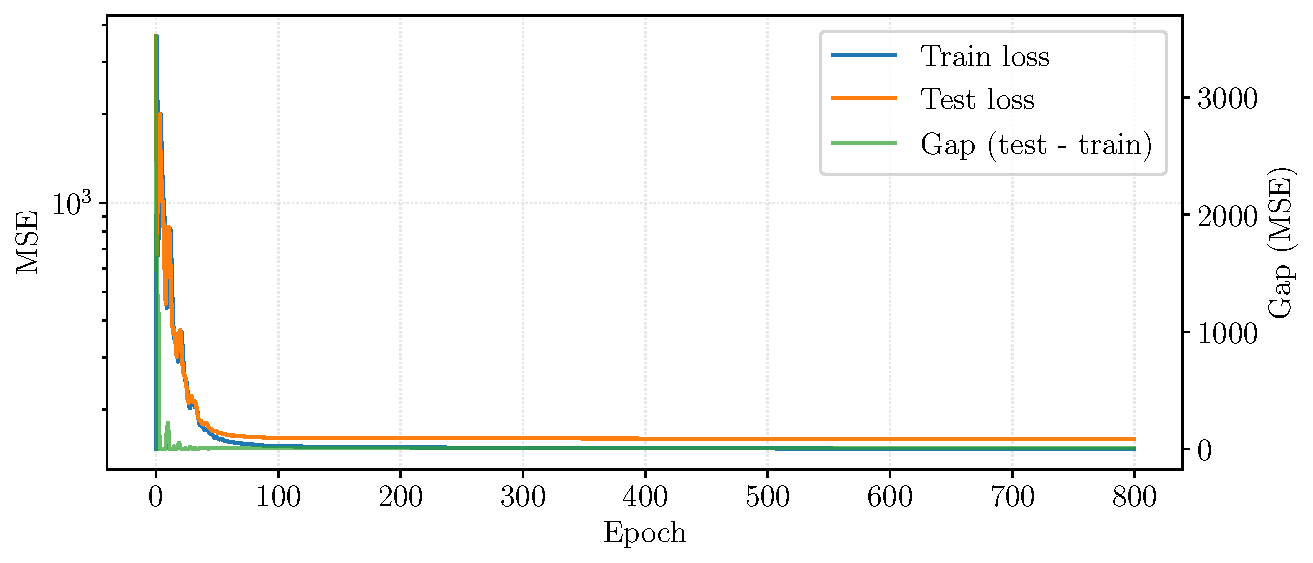
\includegraphics[width=1\linewidth]{Images/epoches_evolution.pdf}}\label{log_b} \\
  \subfloat[\footnotesize Predicted vs true flows using the surrogate model]{
  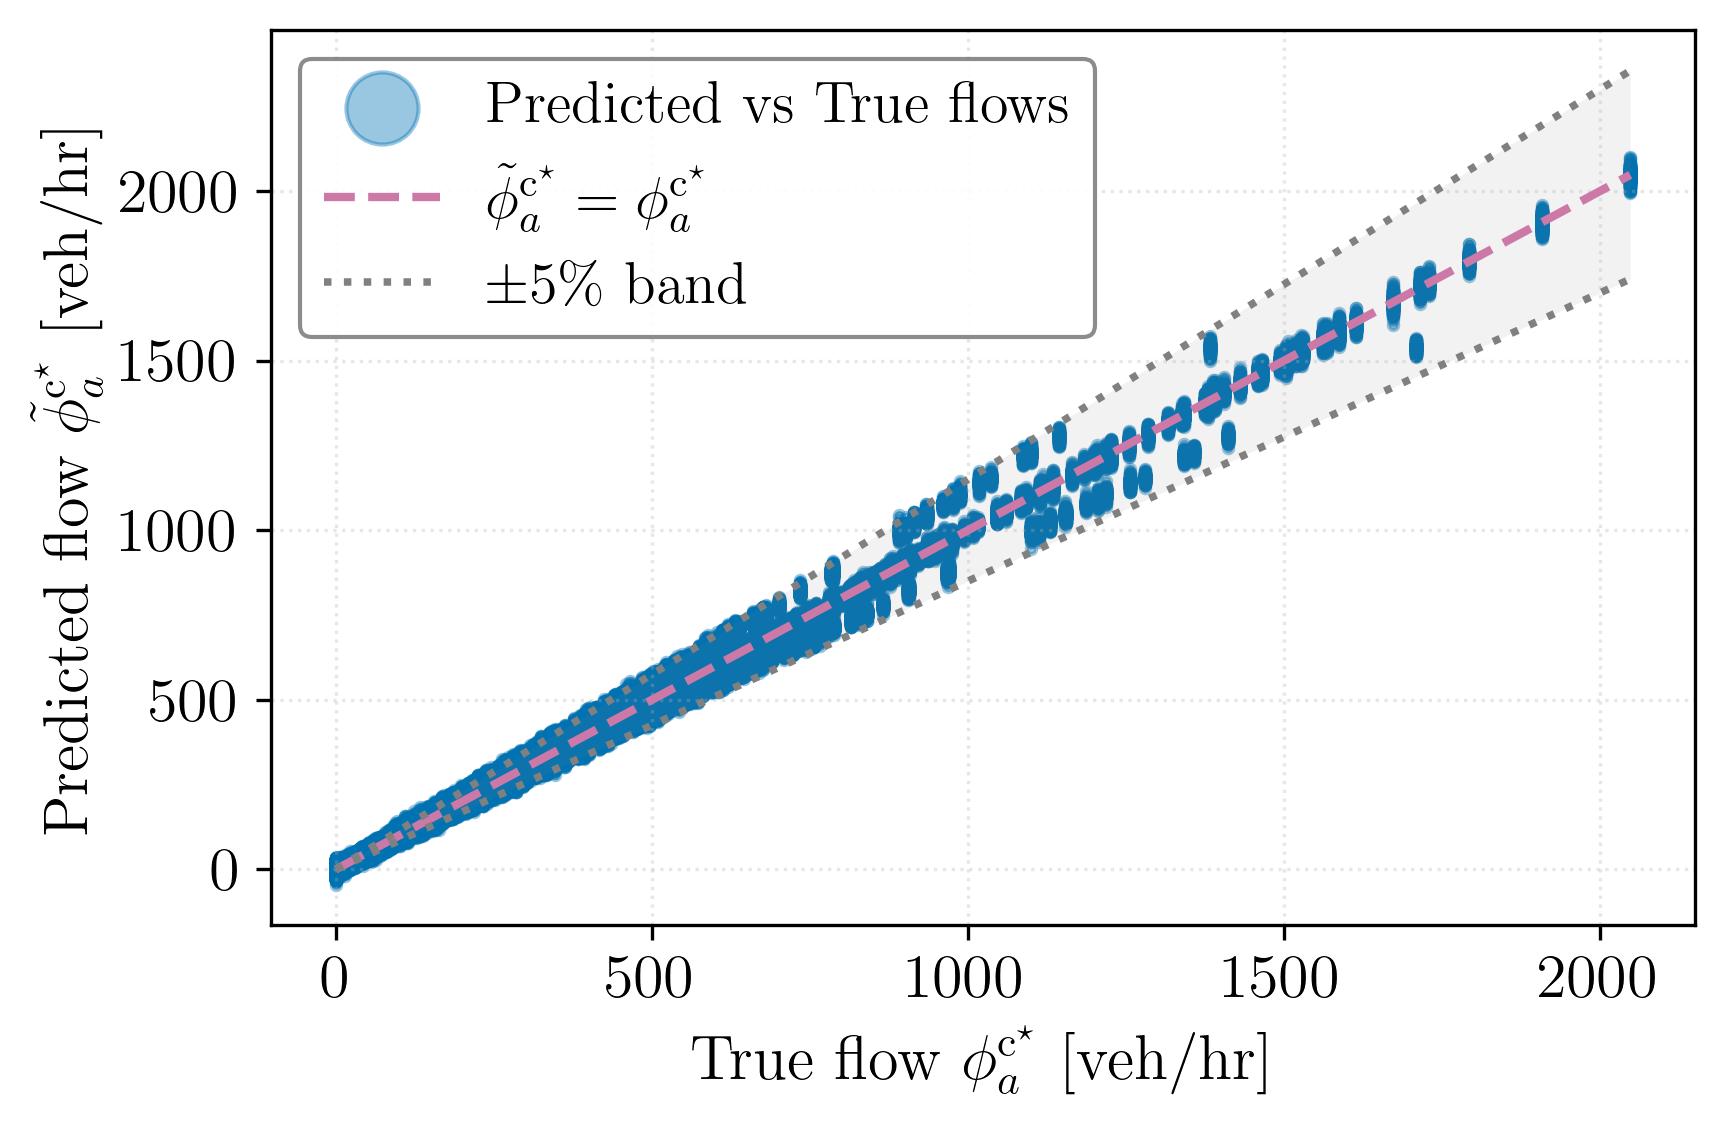
\includegraphics[width=0.9\linewidth]{Images/parity_plot_labeled.png}}\label{log_c}
  \caption{\footnotesize On the top we present the epochs evolution with the 912 samples created for solving Problem~1 and on the bottom how the predicted flows approaches the true flow found by the UE.}
  \label{prediction_model}
\end{figure}
 
 Let $B_{\text{max}}$ represent the budget required to upgrade the entire network to DoS $=6$. The cost per meter $\pi(w_a^\mathrm{b}, \tilde{w}_a^\mathrm{b})$ of upgrading arc $a$ from $w_a^\mathrm{b}$ to $\tilde{w}_a^\mathrm{b}$ is given by the matrix below. The total cost of upgrading an arc is computed as $d_a^\mathrm{b} \cdot \pi(w_a^\mathrm{b}, \tilde{w}_a^\mathrm{b})$, where $d_a^\mathrm{b}$ is the arc length, making the cost distance-dependent. The cost matrix $\Pi$ is adapted from Cerema’s reported unit construction costs for cycling
infrastructure upgrades in France~\cite{cerema2024_cost}.
\renewcommand{\arraystretch}{0.8} % Reduce row height
\setlength{\tabcolsep}{3pt} % Reduce column spacing
\begin{equation}
  \Pi =
  \scriptsize
  \begin{pmatrix} % Brackets like pmatrix
    \tilde{w}_{a} \textbackslash w_{a} & 1 & 2 & 3 & 4 & 5 & 6 \\ \hline
    1 \quad      \vert & 0\text{€}   & 150\text{€}  & 250\text{€}  & 300\text{€}  & 500\text{€}  & 750\text{€}  \\
    2 \quad   \vert & 0\text{€}   & 0\text{€}    & 100\text{€}  & 150\text{€}  & 350\text{€}  & 600\text{€}  \\
    3 \quad  \vert & 0\text{€}   & 0\text{€}    & 0\text{€}    & 50\text{€}   & 250\text{€}  & 500\text{€}  \\
    4 \quad  \vert & 0\text{€}   & 0\text{€}    & 0\text{€}    & 0\text{€}    & 200\text{€}  & 450\text{€}  \\
    5 \quad  \vert & 0\text{€}   & 0\text{€}    & 0\text{€}    & 0\text{€}    & 0\text{€}    & 250\text{€}  \\
    6 \quad \vert& 0\text{€}   & 0\text{€}    & 0\text{€}    & 0\text{€}    & 0\text{€}    & 0\text{€}    \\
  \end{pmatrix}
\end{equation}
% According to the investment plan for Grenoble of March 2025 \cite{GrenobleMetropole2025} the investments for the cycling network of Grenoble and are around 24.5M \text{€}, that is $B \approx 0.15 \cdot B_{\max}$, then we solve Problem~2 and Problem~3 for that budget, and for ten different values of $\epsilon~\in~\Lambda = \left\{ 0, \frac{1}{10}, \frac{1}{5}, \frac{3}{10}, \mathrm{40 \%}, \frac{1}{2}, \frac{3}{5}, \frac{7}{10}, \frac{4}{5}, \frac{9}{10}, 1 \right\}$, where $\Lambda$ is called the set of $\epsilon$-constraints. For each $B$, we solve Problem~1 for every $\epsilon \in \Lambda$ and evaluate the resulting set $\left\{ (\epsilon \cdot \mathcal{E}, (1 - \epsilon) \cdot \mathcal{T}) \right\}_{\epsilon \in \Lambda}$. For the utilitarian case (Problem~2), the optimal trade-off between cyclist exposure and total travel time is defined as the point on the Pareto front with the shortest Euclidean distance to the origin
% \begin{equation}
% \label{opt_trade_off_ut}
%     \epsilon^{\star} = \arg\min_{\epsilon \in \Lambda} \sqrt{ \left( \epsilon \cdot J_{\mathcal{E}} \right)^2 + \left( (1 - \epsilon) \cdot \hat{\mathcal{T}} \right)^2 }.
% \end{equation}
% And similarly for Problem~3 $\epsilon \in \Lambda$ and evaluate the resulting set $\left\{ (\epsilon \cdot J_{\mathrm{SI}}, (1 - \epsilon) \cdot \left [J_{\mathrm{TI}}^\mathrm{b} + J_{\mathrm{TI}}^\mathrm{c} \right ]) \right\}_{\epsilon \in \Lambda}$. For the sufficientarian perspective, the optimal trade-off between cyclist exposure-based path insufficiency and travel time insufficiency is defined as the point on the Pareto front with the shortest Euclidean distance to the origin
% \begin{equation}
% \label{opt_trade_off}
%     \epsilon^{\star}_{\lambda} = \arg\min_{\epsilon \in \Lambda} \sqrt{ \left( \epsilon \cdot J_{\mathrm{SI}} \right)^2 + \left( (1 - \epsilon) \cdot \left [J_{\mathrm{TI}}^\mathrm{b} + J_{\mathrm{TI}}^\mathrm{c} \right ] \right)^2 }.
% \end{equation}
% Fig.~\ref{pareto_front} presents the results obtained by the two optimization processes: utilitarian for the utilitarian formulation and the sufficientarian formulation for the sufficientarian one. 
% Each point represents a trade-off value of 
% $\left( \epsilon \cdot \mathcal{E},\, (1 - \epsilon) \cdot \mathcal{T} \right)$. 
% When $\epsilon = 0$, utilitarian and the sufficientarian formulation focus entirely on minimizing either the total system travel time or the total accessibility unfairness, yielding the lowest overall travel times and the smallest bicycle–car time accessibility unfairness. Conversely, when $\epsilon = 1$, the algorithms focus exclusively on minimizing cyclist exposure and safety-path insufficiency, resulting in the highest overall travel times. The Pareto fronts associated with a budget of $\lambda = \mathrm{10\%}$ are generally shifted leftward compared to those with higher relative path-exposure-based path-protection thresholds ($\mathrm{40\%}$ and $\tfrac{1}{3}$). This indicates that, under lower exposure-based path-protection thresholds, greater improvements in safe-path bicycle infrastructure can be achieved with smaller impacts on car travel times. In contrast, the budget $\alpha = \mathrm{50\%}$ achieves the least reduction in cyclist safety-path insufficiency but induces the largest increase in travel times, as it disrupts the car network the most. The optimal trade-off points from Eq.~\eqref{opt_trade_off} are
% $\epsilon^{\star}_{\mathrm{10\%}} = \epsilon^{\star}_{\mathrm{20\%}} = \mathrm{90\%}$,
% $\epsilon^{\star}_{\tfrac{1}{3}} = \tfrac{8}{10}$,
% $\epsilon^{\star}_{\mathrm{40\%}} = \mathrm{70\%}$,
% and $\epsilon^{\star}_{\mathrm{50\%}} = \mathrm{10\%}$. To illustrate this, Fig.~\ref{individual_pareto} shows the normalized individual metrics for each $\epsilon \in \Lambda$ with $\lambda = \mathrm{40\%}$. As expected, in the baseline configuration we observe the highest cyclist exposure and safety-path insufficiency (normalized value of 1), and the lowest travel time and time-path insufficiency (normalized value of 0). As $\epsilon$ increases, the focus gradually shifts: smaller $\epsilon$ values correspond to higher cyclist exposure and lower travel times, while larger $\epsilon$ values yield the opposite trend. The optimal $\epsilon^{\star}_{\alpha}$ values are highlighted in red.

According to the Grenoble cycling investment plan (March 2025)~\cite{GrenobleMetropole2025}, the planned budget is about
$24.5$M\,€, which corresponds to $B \approx 0.15\,B_{\max}$.
We therefore solve Problem~2 (utilitarian) and Problem~3 (sufficientarian) under this budget constraint.

For each formulation, we explore the trade-off between the competing objectives by solving the corresponding bi-level problem for a discrete set of weights
\[
\Lambda=\left\{0,\mathrm{10\%},\mathrm{20\%},\ldots, \mathrm{100\%}\right\},
\]
where $\gamma\in\Lambda$ controls the balance between the safety-related term and the travel-time/accessibility-related term.
This yields, for each $\gamma$, one candidate solution and one point on the corresponding Pareto front (reported in Fig.~\ref{pareto_front}).

In the sufficientarian formulation, we additionally test several safety-threshold levels through
\[
\lambda\in\left\{\mathrm{10\%},\mathrm{20\%},\mathrm{30\%},\mathrm{40\%},\mathrm{50\%}\right\},
\]
which define increasingly demanding path-safety requirements.
For each $\lambda$, the algorithm is run for all $\gamma\in\Lambda$, producing a family of trade-off curves.

Because the two objectives are expressed in different units, we do not define an ``optimal'' compromise point (e.g., via Euclidean distance to the origin).
Instead, selecting $\gamma$ is ultimately a policy decision that reflects how decision makers value safety improvements relative to travel-time impacts.
To support interpretation and visualization of the results, we highlight one representative weight $\gamma_\lambda^\star$ for each threshold level $\lambda$,
chosen solely for illustration: $
\gamma^\star_{\mathrm{10\%}}=\mathrm{20\%},\,
\gamma^\star_{\mathrm{20\%}}=\mathrm{30\%},\,
\gamma^\star_{\mathrm{30\%}}=\mathrm{40\%},\,
\gamma^\star_{\mathrm{40\%}}=\mathrm{50\%},\,
\gamma^\star_{\mathrm{50\%}}=\mathrm{60\%}.$ These $\gamma_\lambda^\star$ values are used only to exemplify the behavior of the utilitarian and sufficientarian solutions in subsequent figures and discussion;
they should not be interpreted as mathematically optimal trade-offs.

Fig.~\ref{pareto_front} compares the sets of solutions produced by the utilitarian formulation (Problem~2) and the sufficientarian formulation (Problem~3).
As expected, small $\gamma$ values emphasize minimizing travel-time/accessibility impacts, while large $\gamma$ values emphasize cyclist safety objectives,
typically at the cost of higher travel-time impacts.
Lower safety-threshold levels (smaller $\lambda$) generally allow larger safety gains with smaller impacts on car travel times, whereas higher $\lambda$
values impose stricter requirements and may lead to larger disruptions in the motorized network.


\begin{figure}[t]
\vspace{0.2cm}
  \centering
  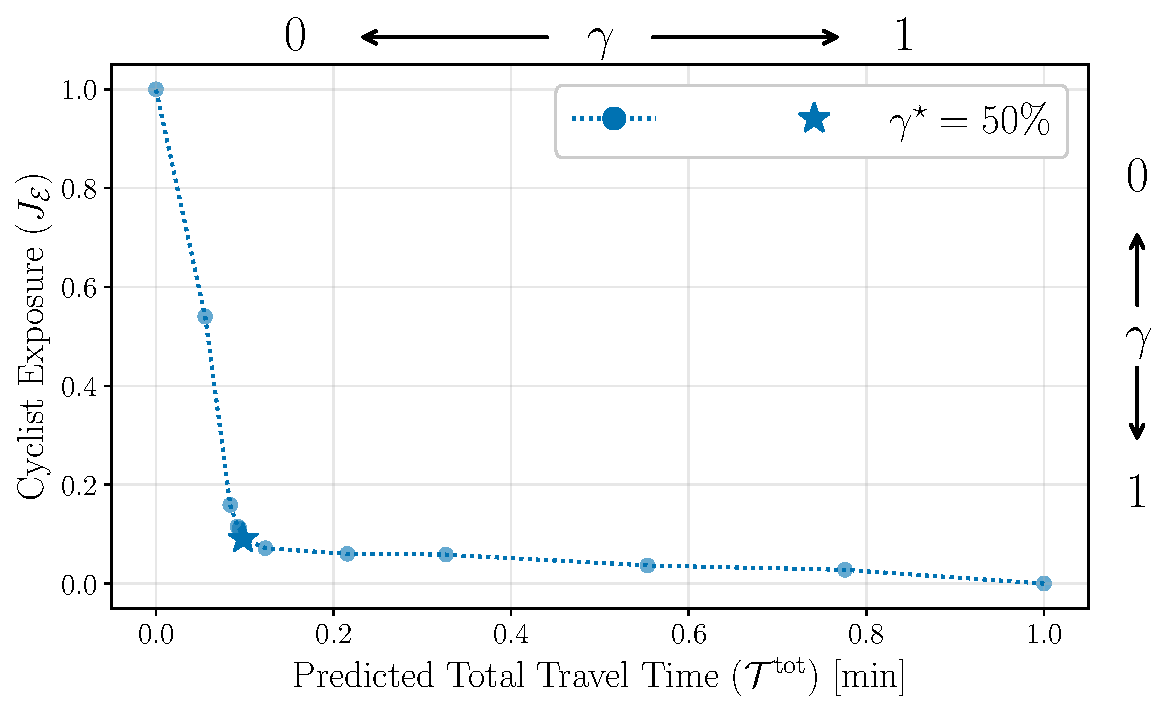
\includegraphics[width=1\linewidth]{Images/pareto_front_swapped_ut.pdf} \\


  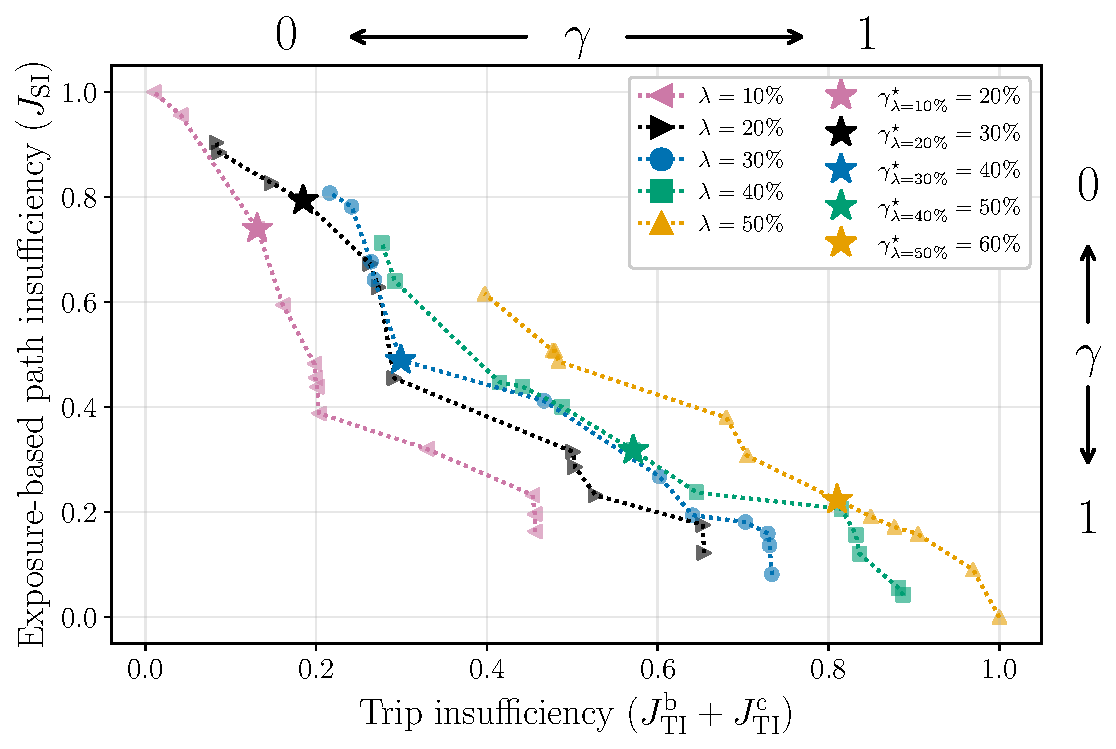
\includegraphics[width=1\linewidth]{Images/pareto_front_swapped_suff.pdf}

  
  \caption{\footnotesize Normalized travel time versus cyclist exposure. 
The top panel shows the Pareto fronts obtained from the trade-off Problem~2 under varying values of $\epsilon \in \Lambda$ and $\alpha \in \Phi$. 
The bottom panel presents the corresponding results for the sufficientarian formulation (Problem~3).}
  \label{pareto_front}
\end{figure}


\begin{figure}[t]
\vspace{0.2cm}
  \centering
  \captionsetup[subfigure]{font={footnotesize}, labelfont={footnotesize, bf}, textfont={footnotesize, rm}}

  \subfloat[\footnotesize Utilitarian perspective]{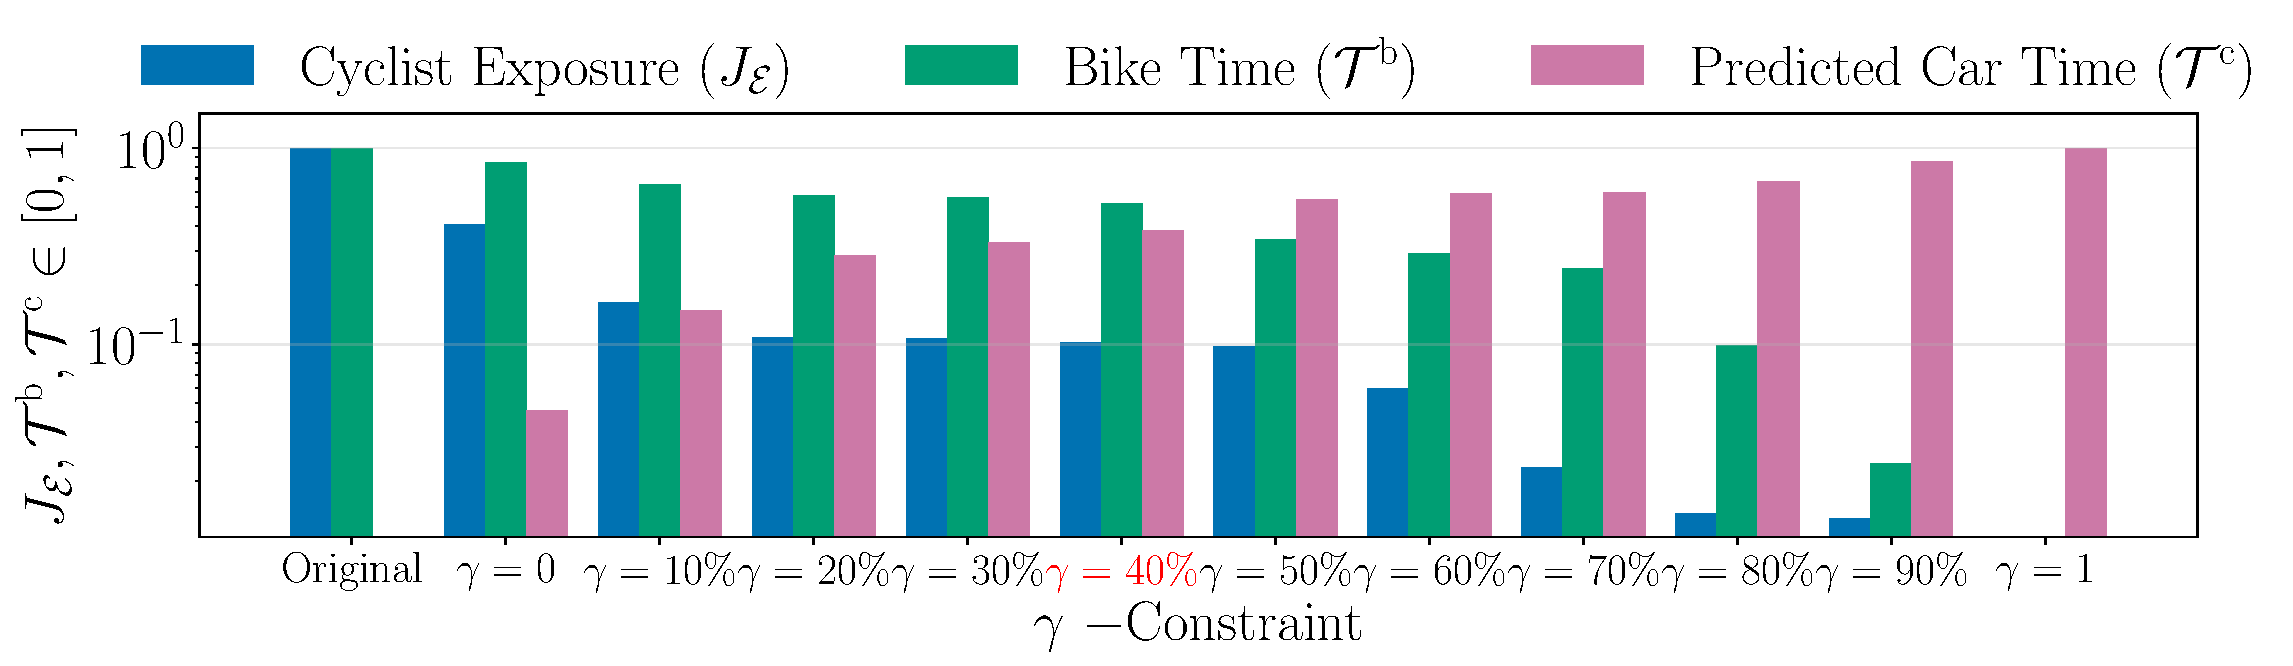
\includegraphics[width=1\linewidth]{Images/exposure_travel_time_comparision_utilitarian.pdf}}\label{ind_ut} \\
  % \subfloat[Sufficientarian perspective $\lambda=\frac{1}{10}$]{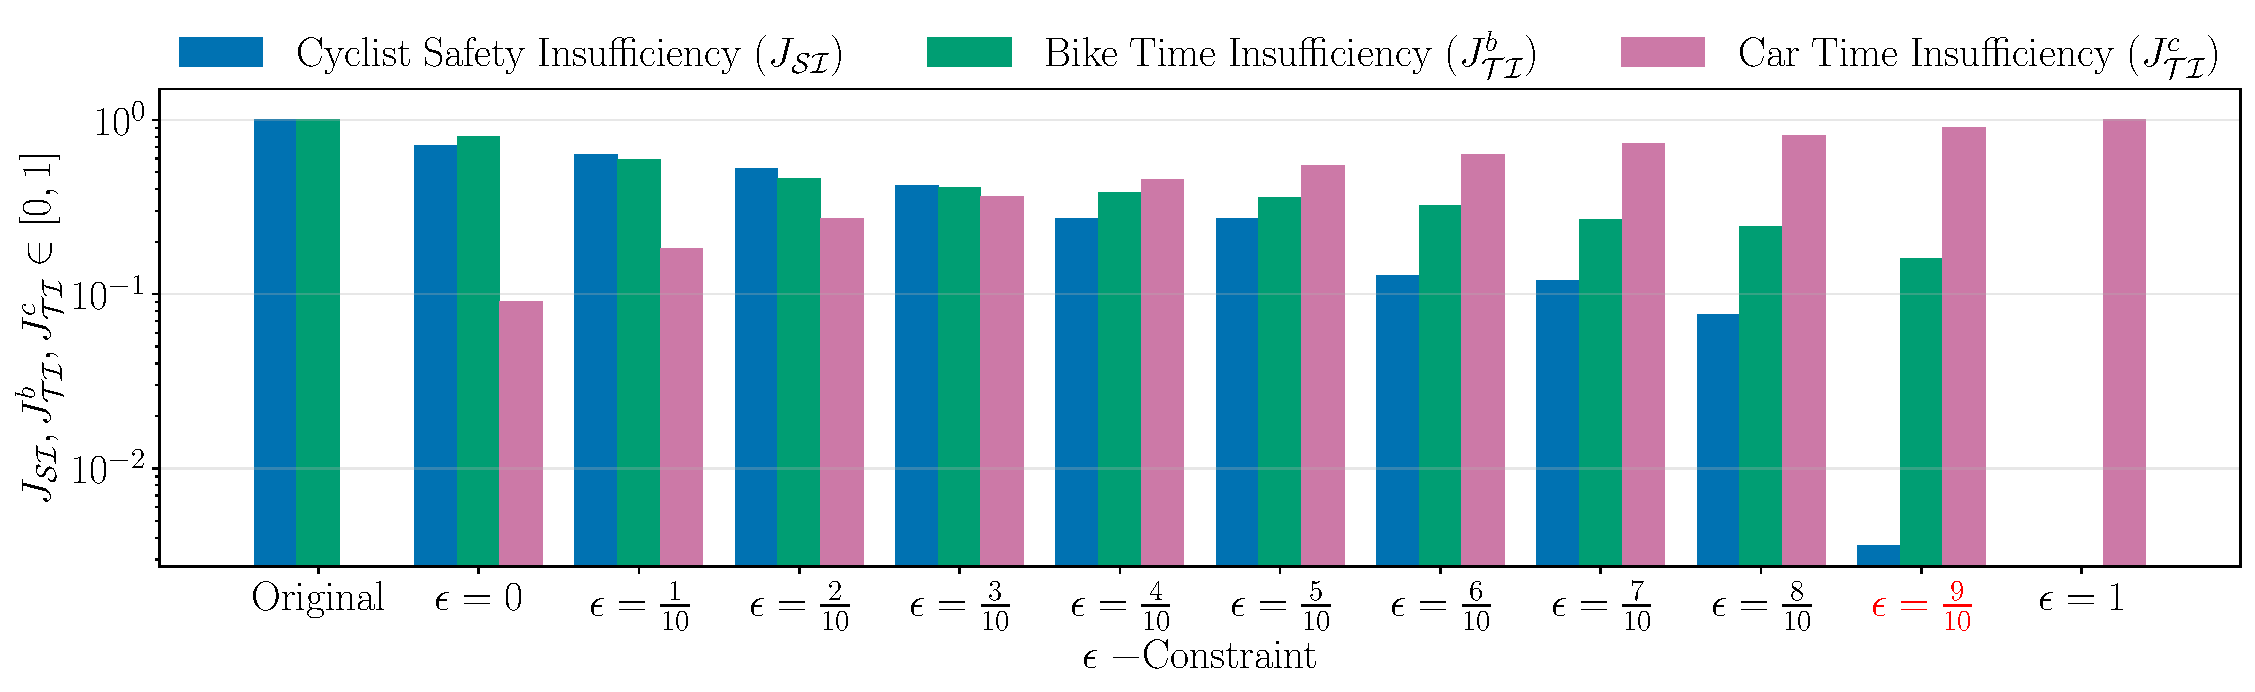
\includegraphics[width=1\linewidth]{Images/exposure_travel_time_comparision_sufficientarian_1_10.pdf}}\label{ind_1_10} \\
  % \subfloat[Sufficientarian perspective $\lambda=\frac{1}{5}$]{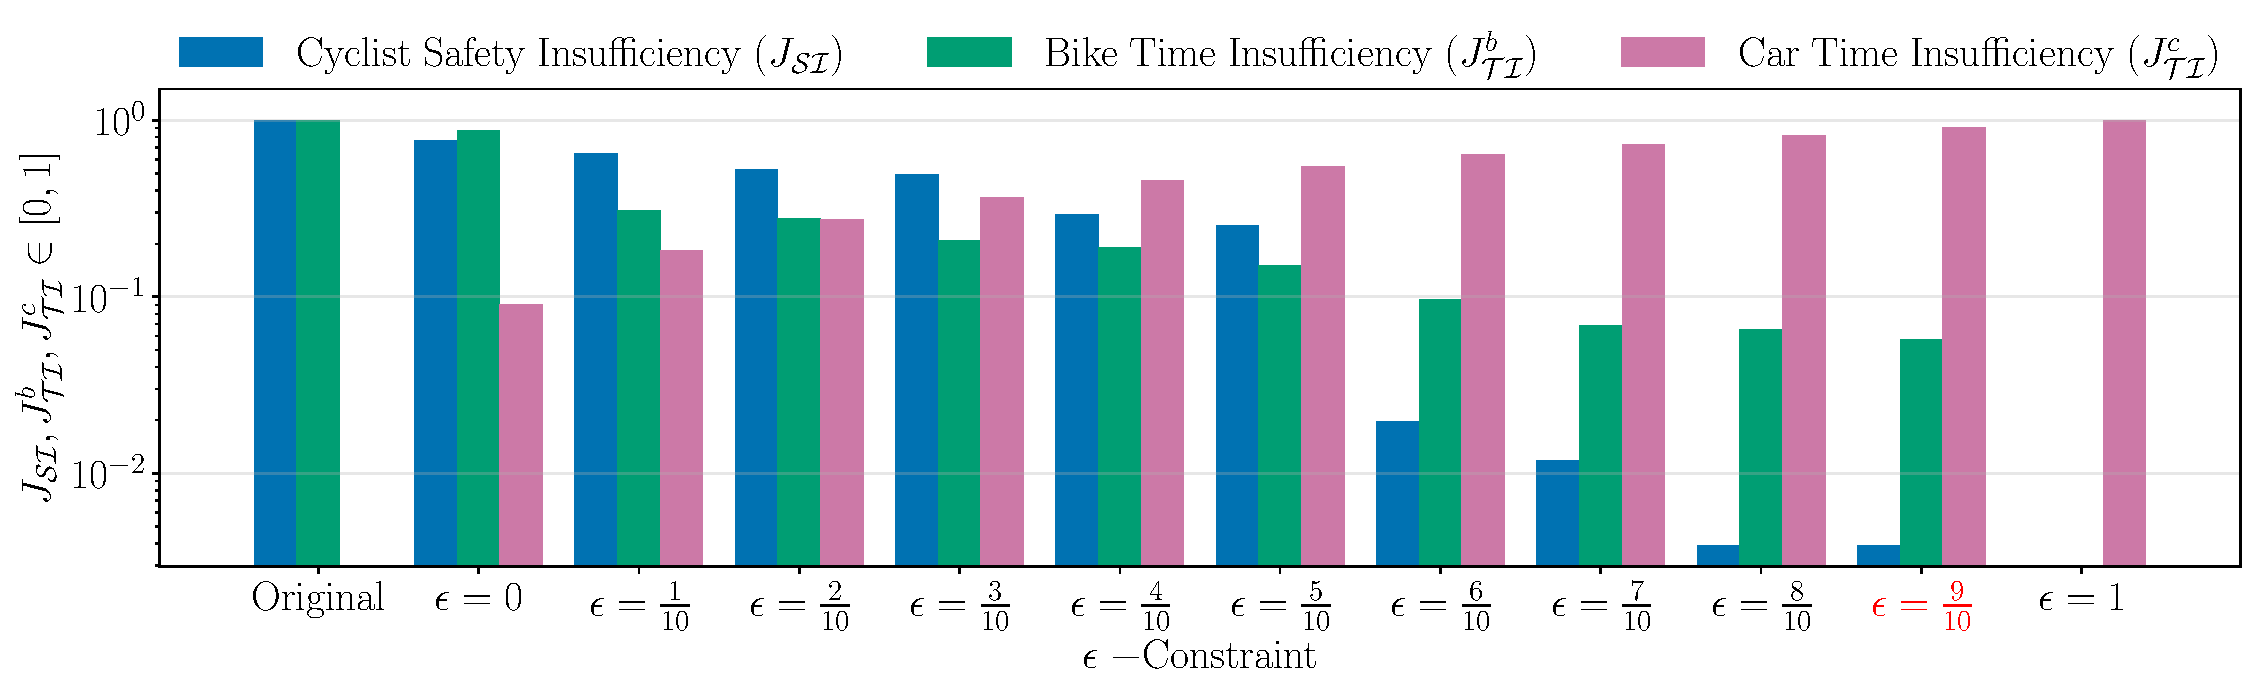
\includegraphics[width=1\linewidth]{Images/exposure_travel_time_comparision_sufficientarian_1_5.pdf}}\label{ind_1_5}\\
  % \subfloat[Sufficientarian perspective $\lambda=\frac{1}{3}$]{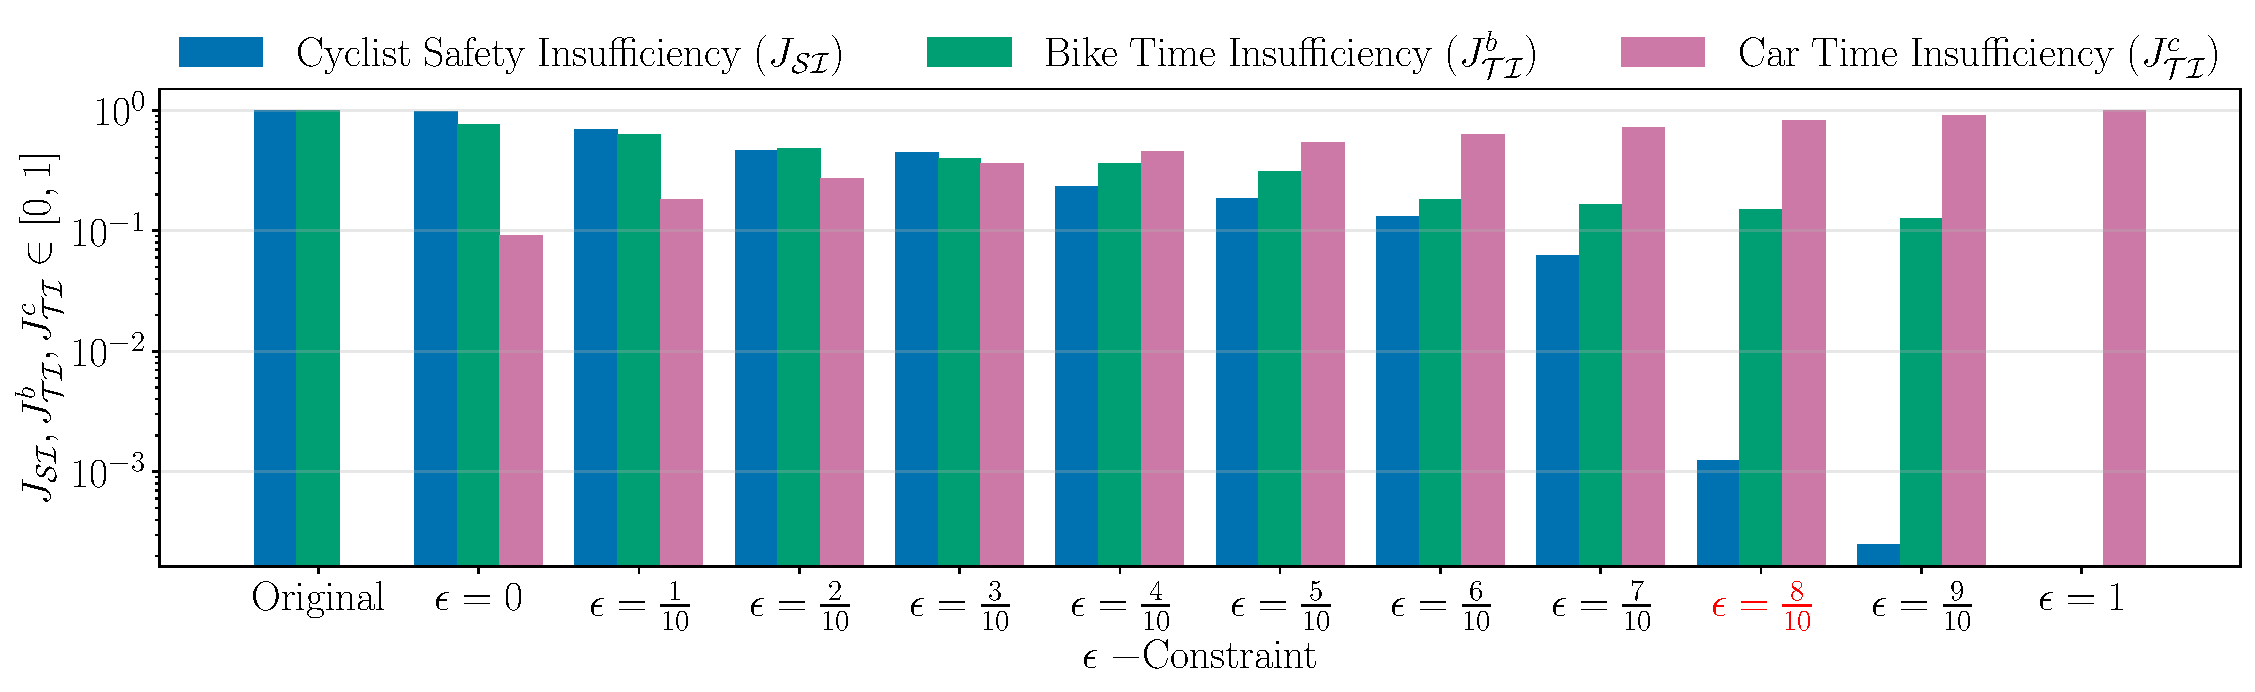
\includegraphics[width=1\linewidth]{Images/exposure_travel_time_comparision_sufficientarian_1_3.pdf}}\label{ind_1_3} \\
  \subfloat[\footnotesize Sufficientarian perspective $\lambda=\mathrm{40 \%}$]{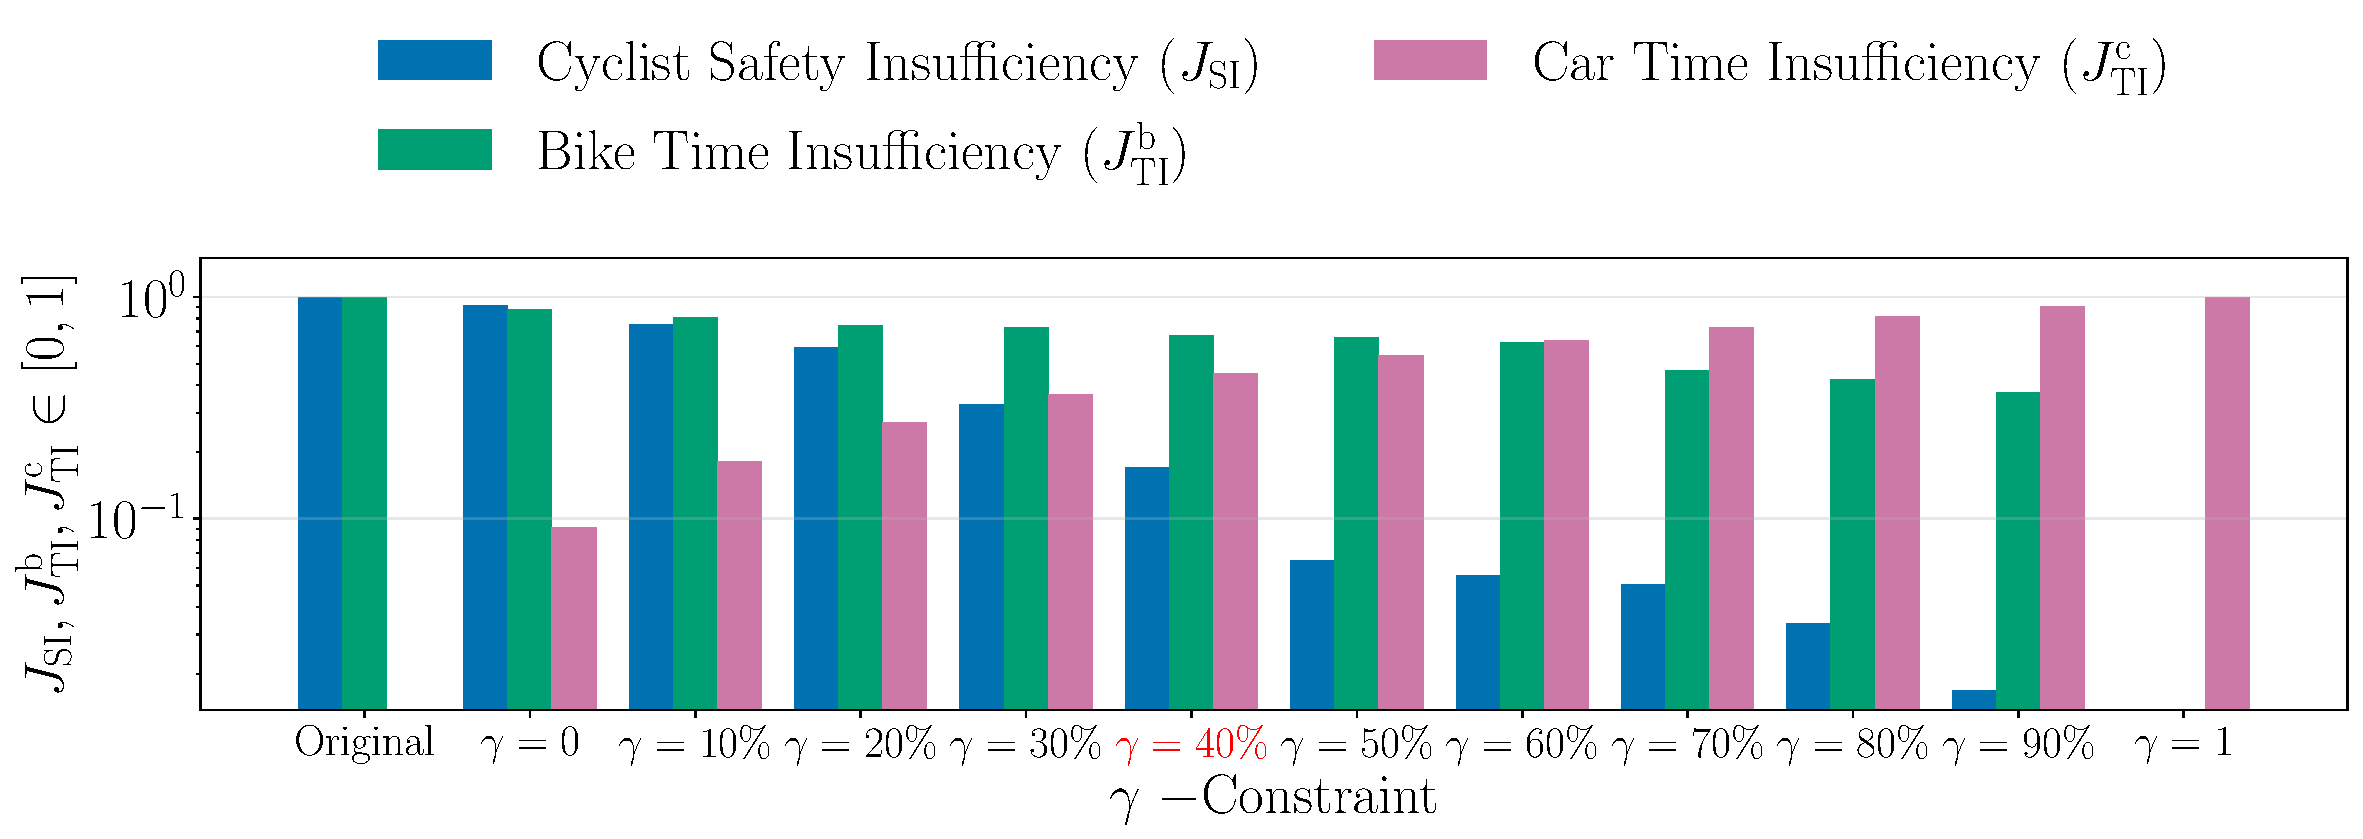
\includegraphics[width=1\linewidth]{Images/exposure_travel_time_comparision_sufficientarian_2_5.pdf}}\label{ind_2_5}
  % \subfloat[Sufficientarian perspective $\lambda=\frac{1}{2}$]{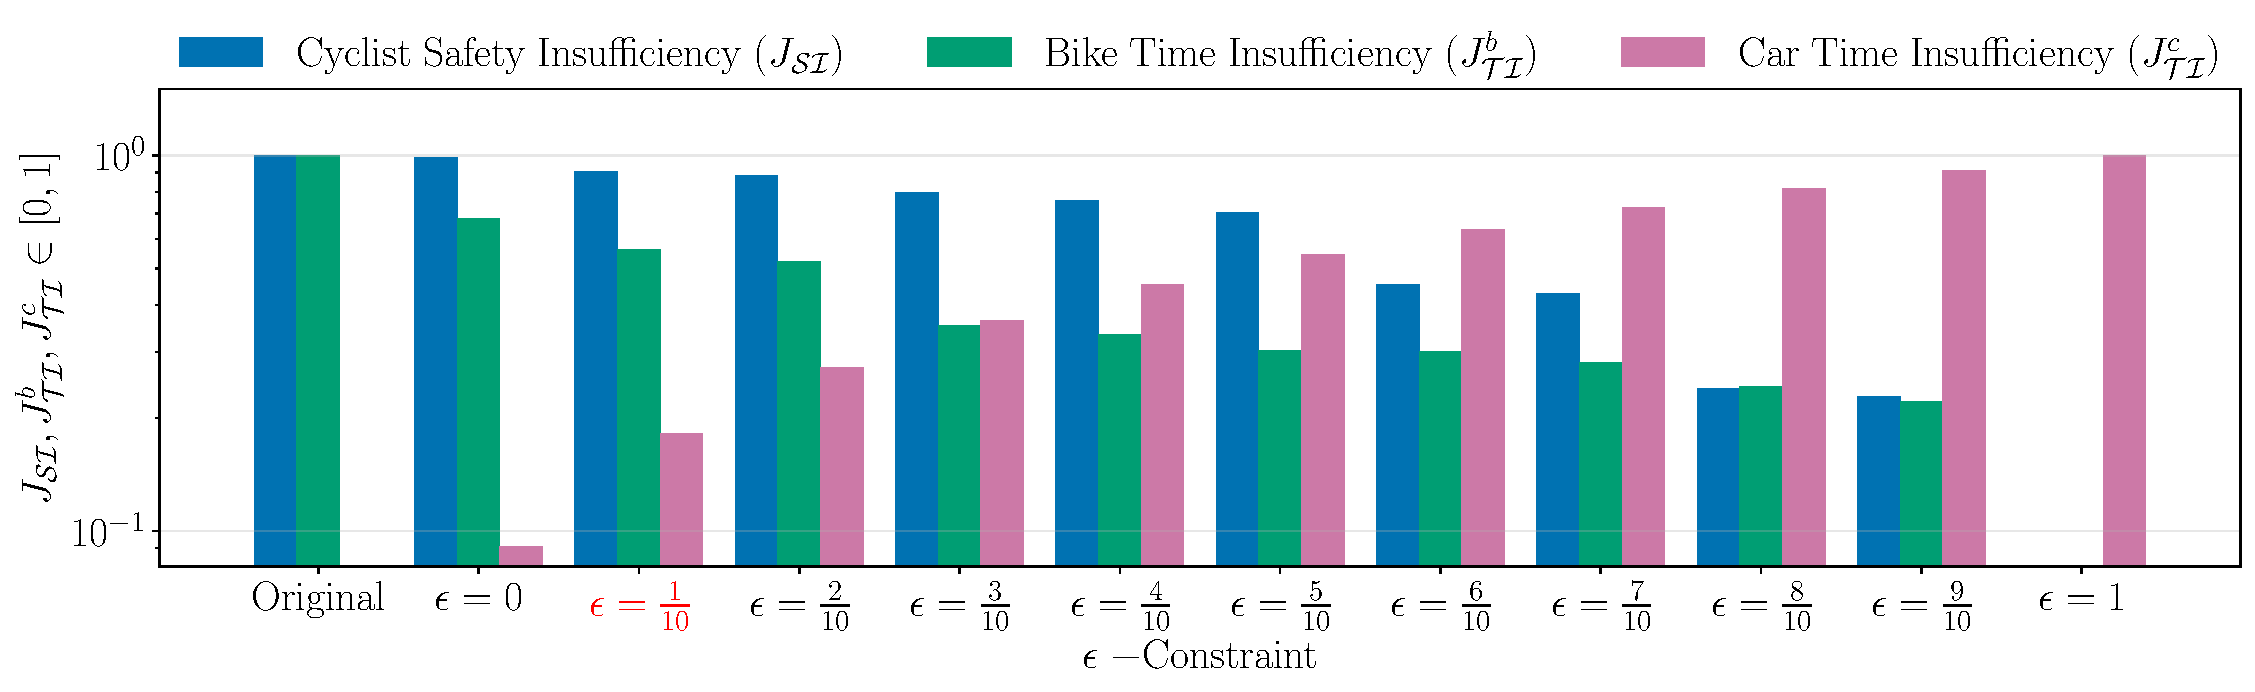
\includegraphics[width=1\linewidth]{Images/exposure_travel_time_comparision_sufficientarian_1_2.pdf}}\label{ind_1_2}
  
  \caption{\footnotesize Normalized cyclist exposure, travel time, safety path insufficiency, cyclist and drivers trip insufficiency trade-off for $\lambda = \mathrm{40 \%}$.}
  \label{individual_pareto}
\end{figure}
\begin{figure}[h!]
\vspace{0.2cm}
\centering

\begin{minipage}{0.99\linewidth}
    \centering
    \textbf{(a) Original}\par\vspace{0.03cm}
    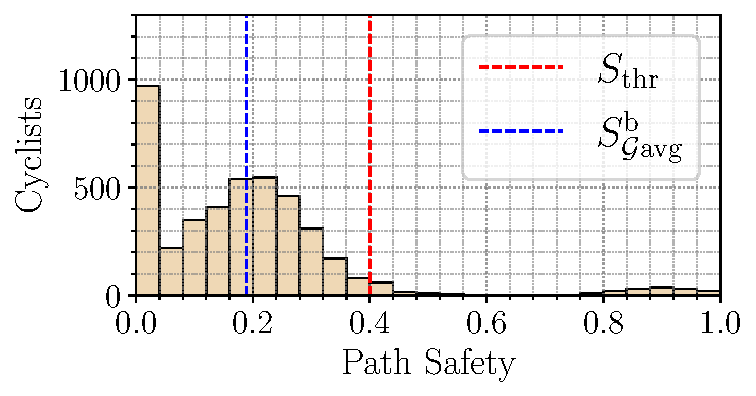
\includegraphics[width=\linewidth]{Images/path_safety_original_only.pdf}
\end{minipage}

\vspace{0.12cm}

\begin{minipage}{0.99\linewidth}
    \centering
    \textbf{(b) Utilitarian}\par\vspace{0.03cm}
    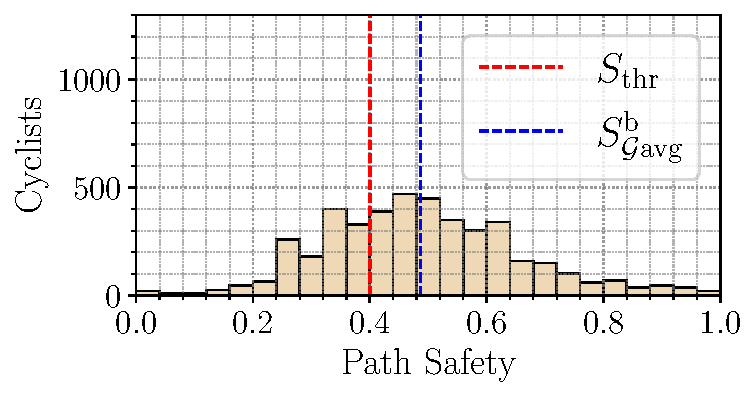
\includegraphics[width=\linewidth]{Images/path_safety_gau_only.pdf}
\end{minipage}

\vspace{0.12cm}

\begin{minipage}{0.99\linewidth}
    \centering
    \textbf{(c) Sufficientarian}\par\vspace{0.03cm}
    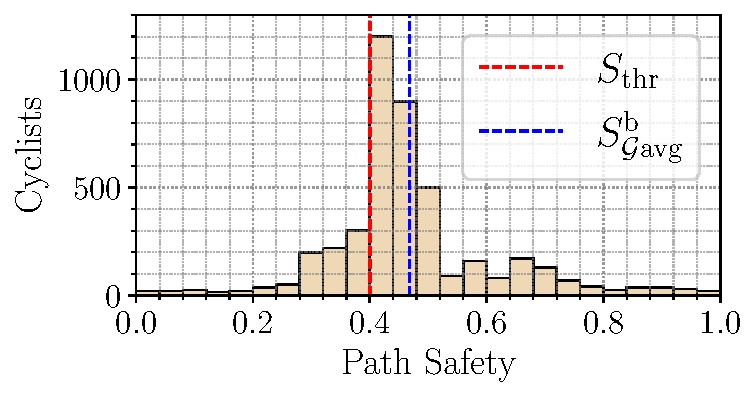
\includegraphics[width=\linewidth]{Images/path_safety_gas_only.pdf}
\end{minipage}

\caption{\footnotesize Exposure-based path-sufficiency score versus the number of cyclists above and below the threshold $\lambda = \mathrm{40\%}$ under a budget of $B$. The dashed red and blue lines indicate the path-sufficiency threshold
$s_{\mathrm{thr}}$ and the average exposure-based path-sufficiency score
$S^{\mathrm{b}}_{\mathcal{G}_{\mathrm{avg}}}$, respectively.}
\label{histograms_plots}
\end{figure}
\begin{figure}[h!]
\vspace{0.2cm}
\centering

\begin{minipage}{0.99\linewidth}
    \centering
    \textbf{(a) Original}\par\vspace{0.03cm}
    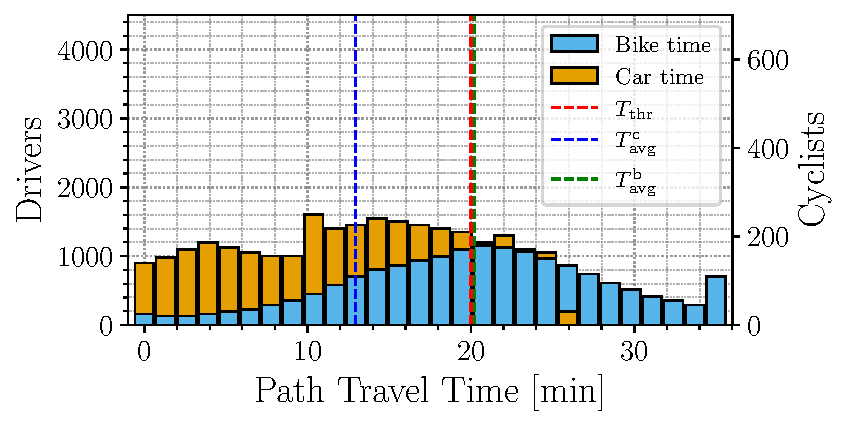
\includegraphics[width=\linewidth]{Images/travel_time_original_only.pdf}
    \label{hist_1_t}
\end{minipage}

\vspace{0.12cm}

\begin{minipage}{0.99\linewidth}
    \centering
    \textbf{(b) Utilitarian}\par\vspace{0.03cm}
    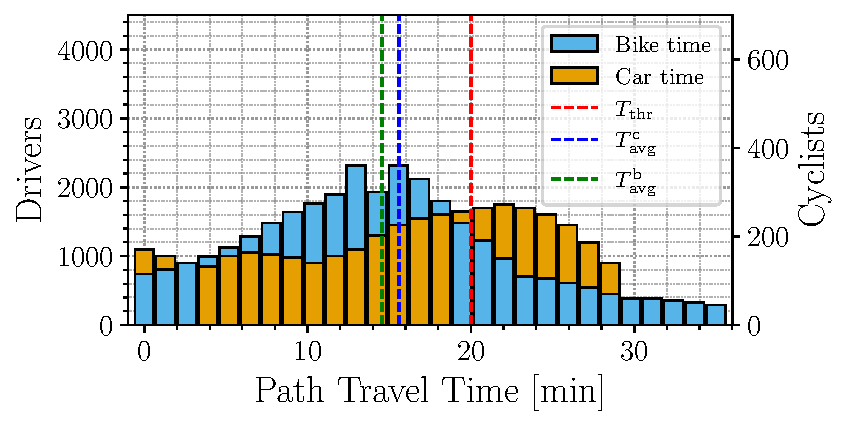
\includegraphics[width=\linewidth]{Images/travel_time_gau_only.pdf}
    \label{hist_3_t}
\end{minipage}

\vspace{0.12cm}

\begin{minipage}{0.99\linewidth}
    \centering
    \textbf{(c) Sufficientarian}\par\vspace{0.03cm}
    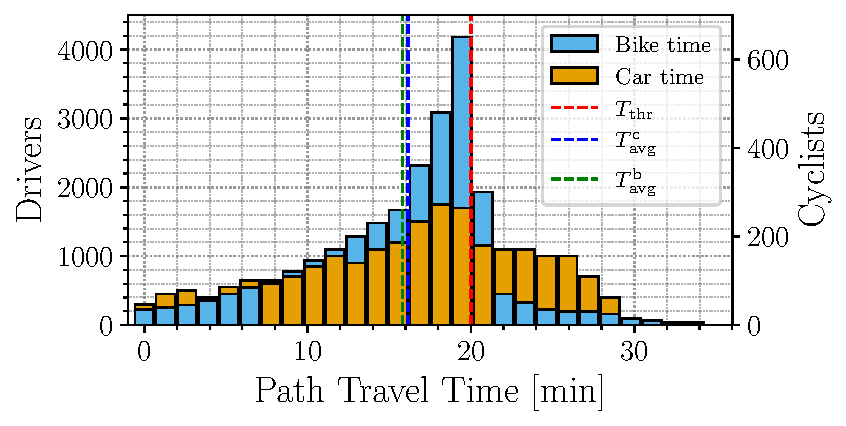
\includegraphics[width=\linewidth]{Images/travel_time_gas_only.pdf}
    \label{hist_4_t}
\end{minipage}

\caption{\footnotesize Drivers (left $y$-axis) and cyclists (right $y$-axis) trip insufficiency versus the number of individuals above and below the threshold $\lambda = \mathrm{40\%}$ under a budget of $B^{\ast}_{\lambda} \approx 0.15 \cdot B_{\max}$ for the different optimization algorithms. The dotted red, blue, and green lines indicate the trip-insufficiency threshold $T_{\mathrm{thr}}$, the average bicycle trip time $T^{\mathrm{b}}_{\mathcal{G}_{\mathrm{avg}}}$, and the average car trip time $T^{\mathrm{c}}_{\mathcal{G}_{\mathrm{avg}}}$ of the entire network, respectively.}
\label{histograms_plots_justice}
\end{figure}



\begin{figure}[t]
\vspace{0.2cm}
  \centering
  \captionsetup[subfigure]{font={footnotesize}, labelfont={footnotesize, bf}, textfont={footnotesize, rm}}

  \subfloat[\footnotesize Exposure-based path insufficiency $\lambda=\mathrm{40 \%}$]{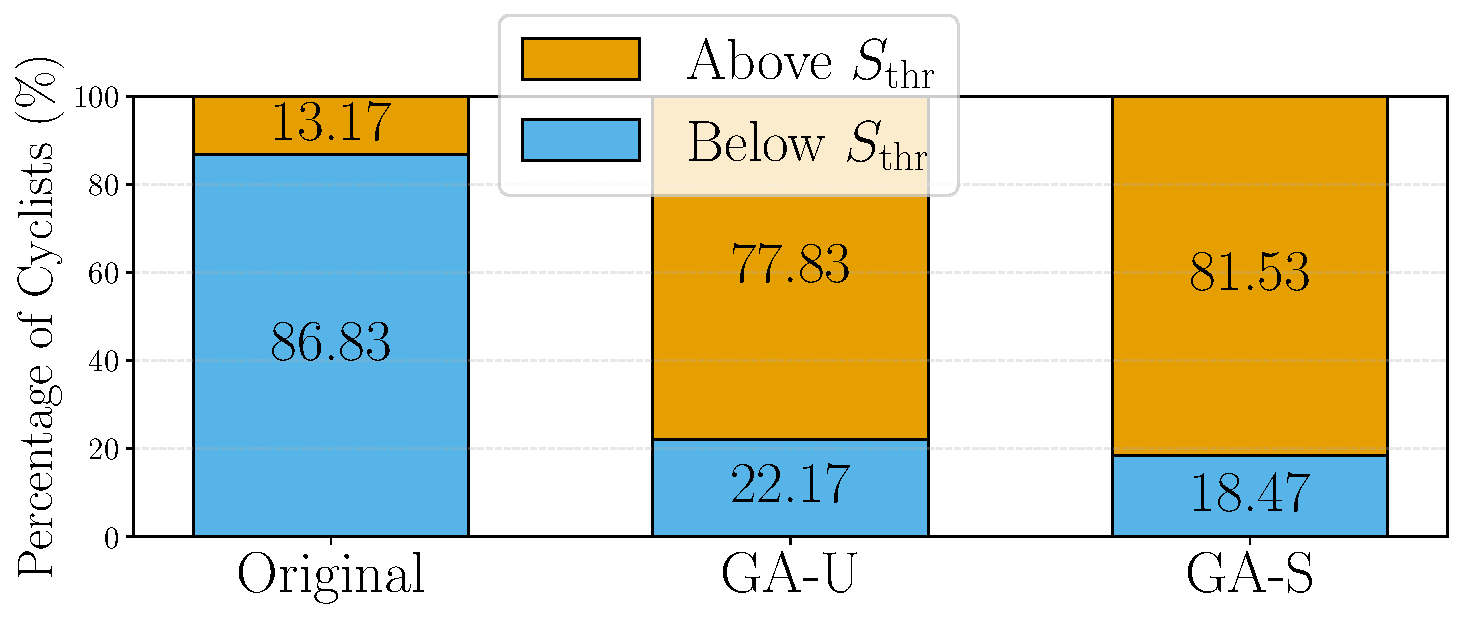
\includegraphics[width=1\linewidth]{Images/percentage_bars_safety_key_0.pdf}}\label{per_saf} \\
  \subfloat[\footnotesize Cyclist trip insufficiency $\lambda=\mathrm{40 \%}$]{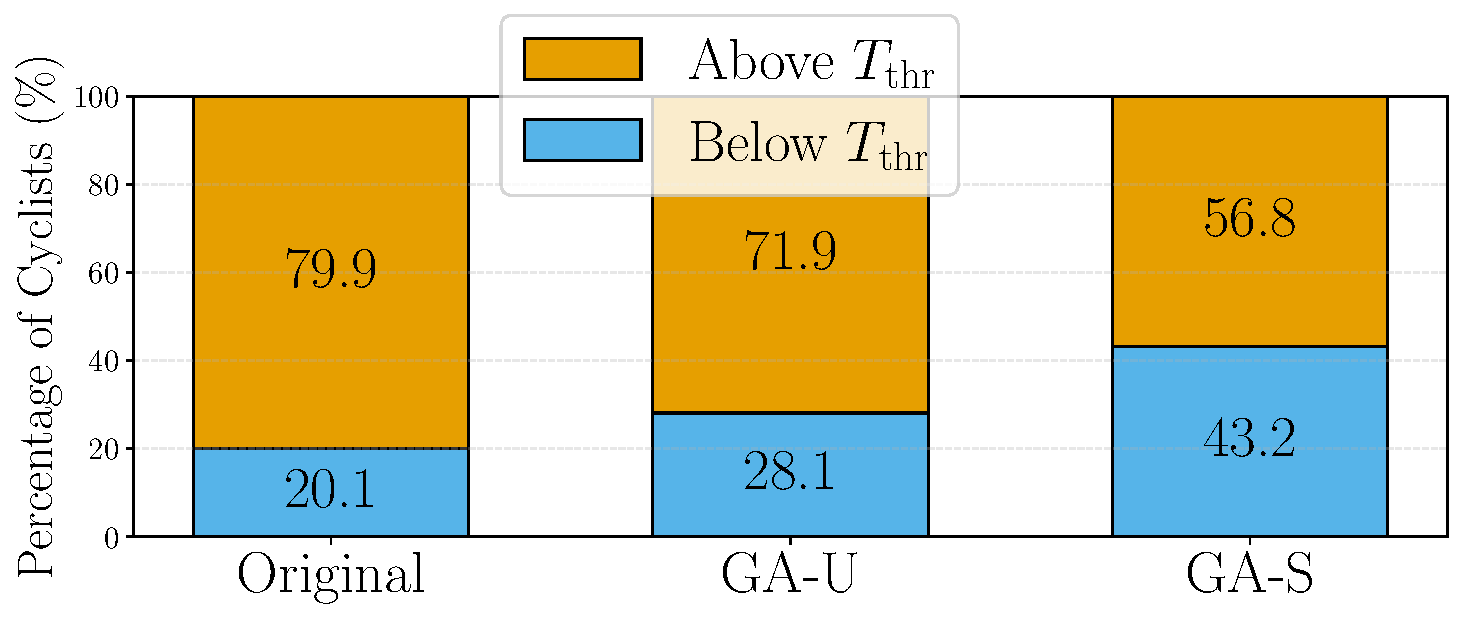
\includegraphics[width=1\linewidth]{Images/percentage_bars_time_key_1.pdf}}\label{per_time} \\
  \subfloat[\footnotesize Drivers trip insufficiency $\lambda=\mathrm{40 \%}$]{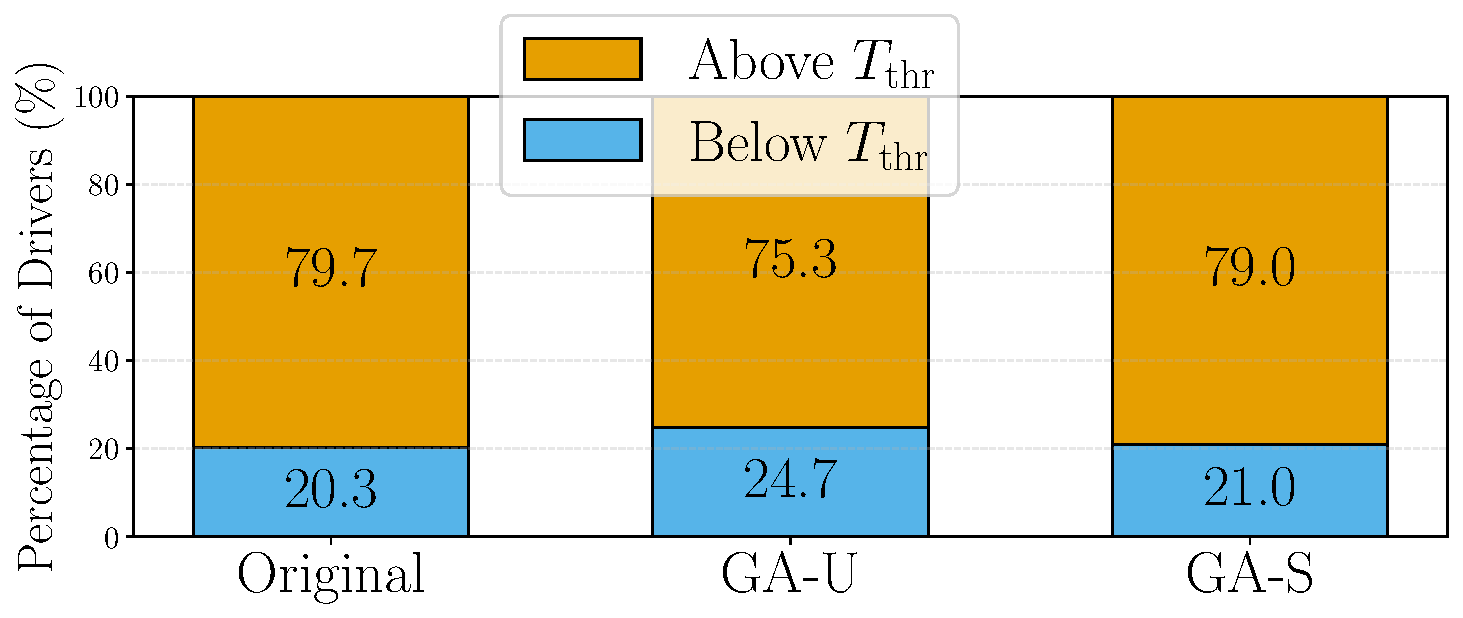
\includegraphics[width=1\linewidth]{Images/percentage_bars_time_cars_key_2.pdf}}\label{per_time_car}
  
  \caption{\footnotesize Normalized exposure-based path insufficiency, bike path-time insufficiency and car path-time insufficiency for $\lambda=\mathrm{40 \%}$.}
  \label{Percentage_thr}
\end{figure}










\subsection{Algorithms Comparison}

\begin{figure*}[!h]
\vspace{0.2cm}
  \centering
  \captionsetup[subfigure]{font={footnotesize}, labelfont={footnotesize, bf}, textfont={footnotesize, rm}}

  \subfloat[Original DoS,  $\overline{D}^\mathrm{b}=4.41$, $P^\mathrm{b} = 16.49$ \%]{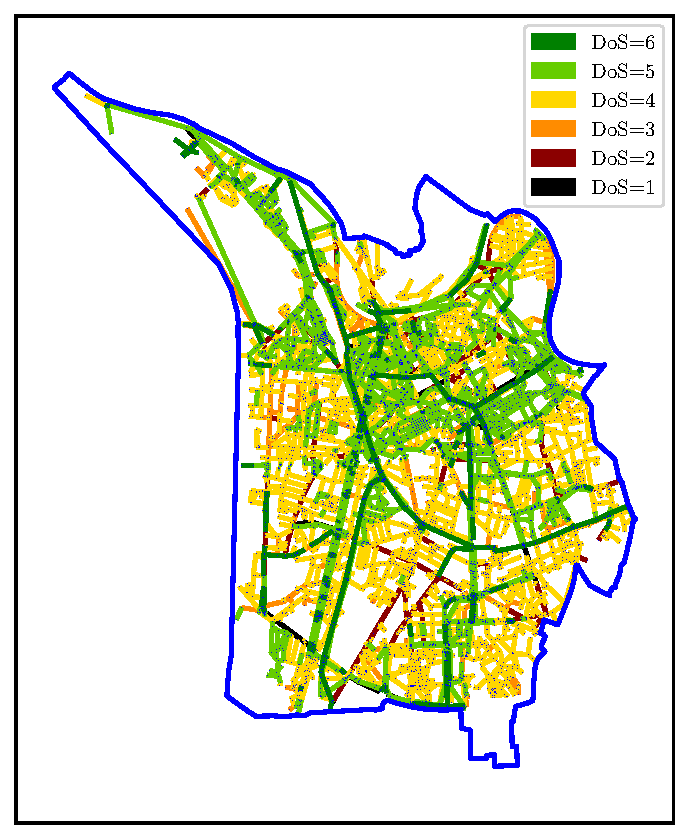
\includegraphics[width=0.23\linewidth]{Images/G_original_DoS_1_2.pdf}\label{1_1}}
  \hspace{0.012\linewidth}
  \subfloat[\mbox{Utilitarian} DoS, $\overline{D}^\mathrm{b}=4.36$, $P^\mathrm{b} = 18.05$ \%.]
  {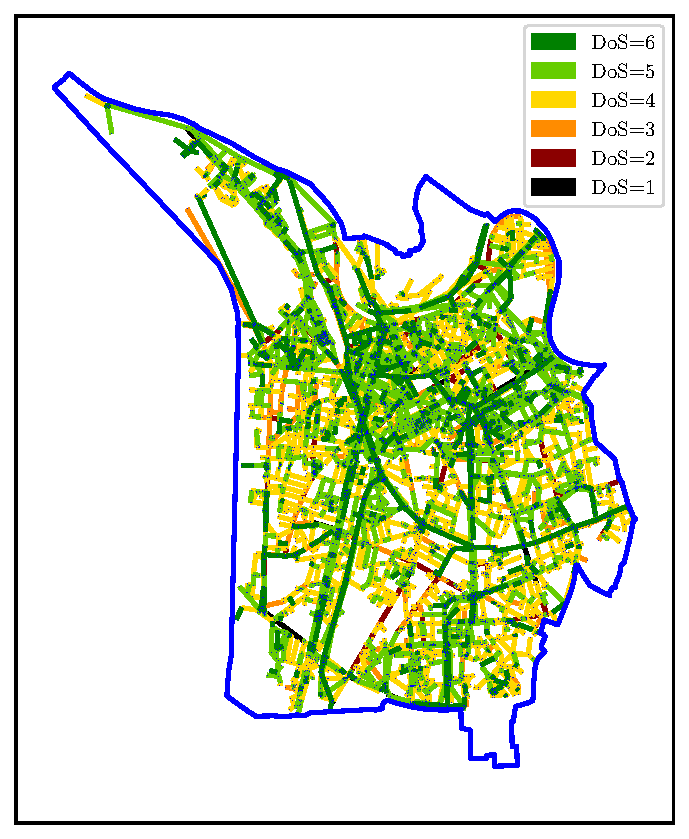
\includegraphics[width=0.23\linewidth]{Images/ut_DoS_1_2.pdf}\label{1_3}}
  \hspace{0.012\linewidth}
  \subfloat[\mbox{Sufficientarian} DoS, $\overline{D}^\mathrm{b}=4.31$, $P^\mathrm{b} = 19.48$ \%.]
  {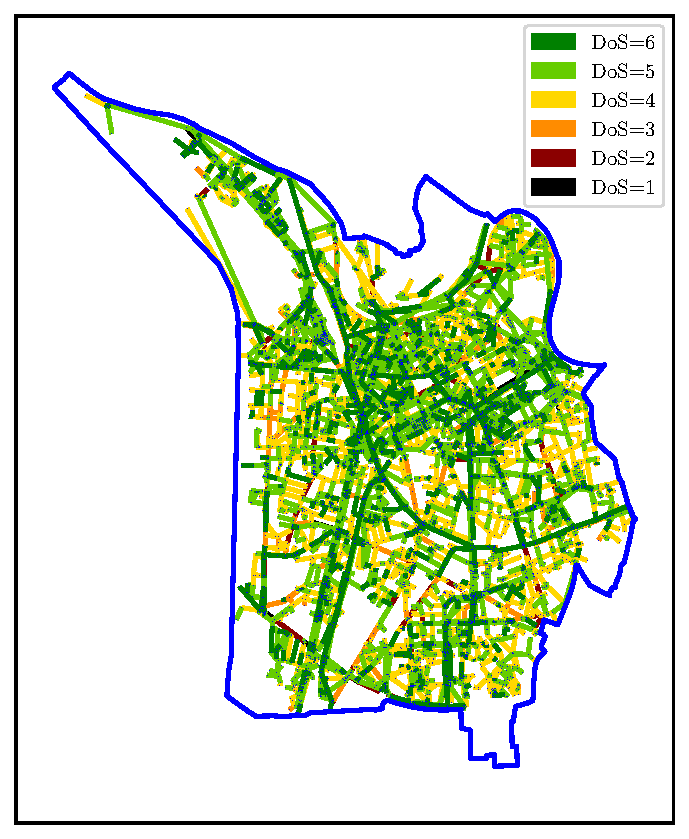
\includegraphics[width=0.23\linewidth]{Images/suff_DoS_1_2.pdf}\label{1_4}}\\
  \subfloat[Original safety path insufficiency]{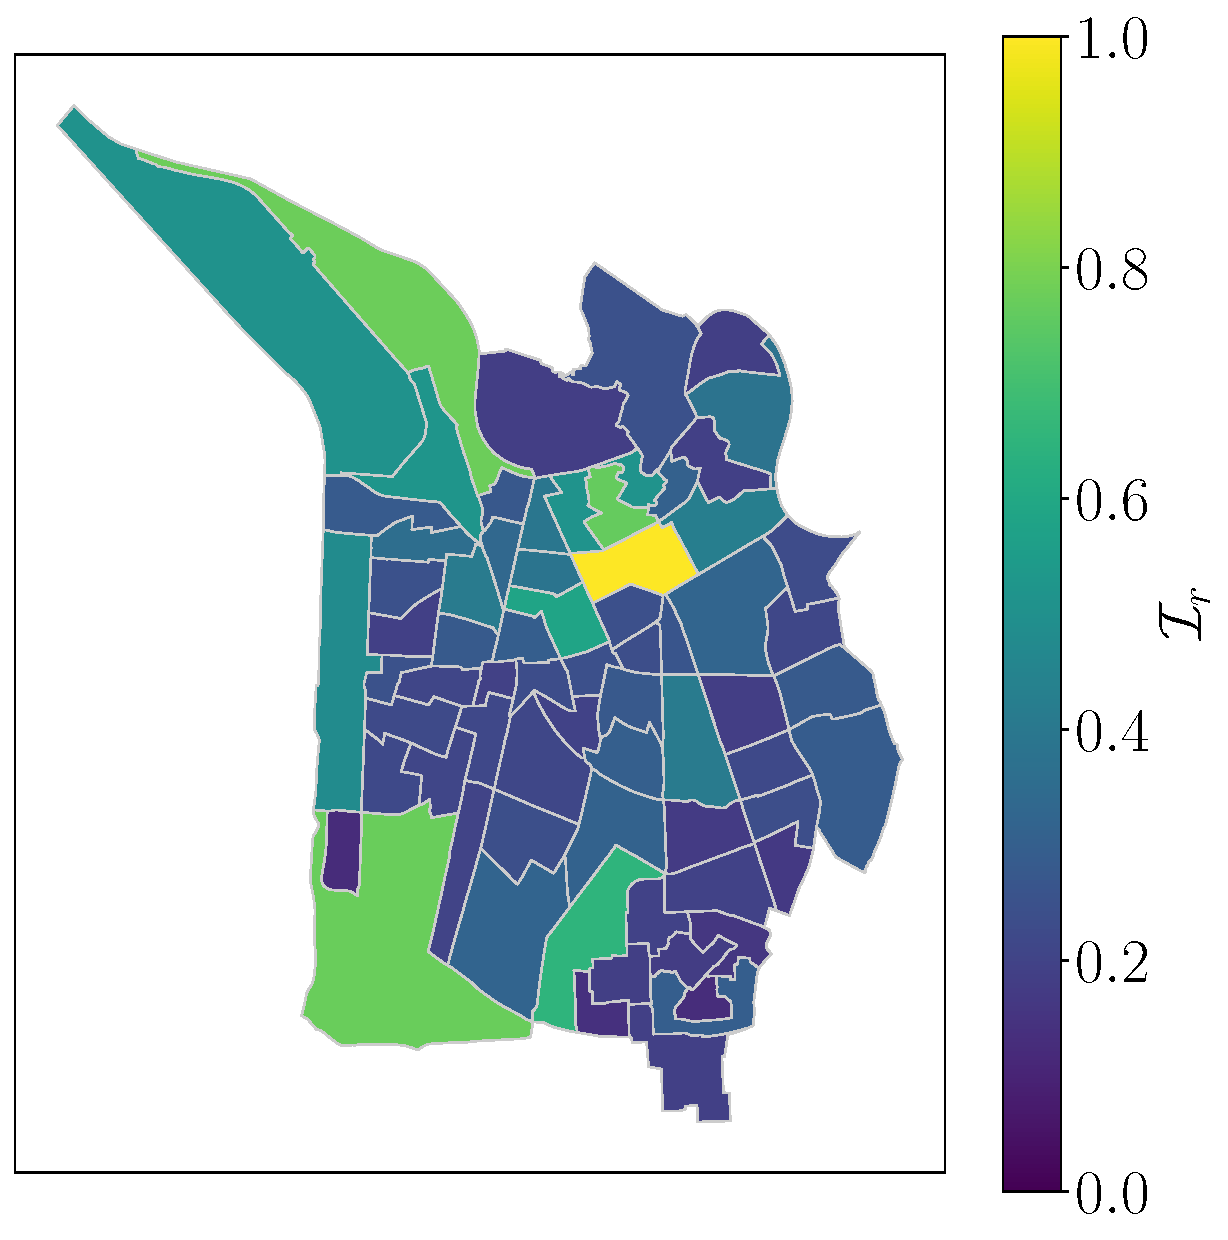
\includegraphics[width=0.24\linewidth]{Images/G_original_regional_1_2.pdf}\label{2_1}}
  \hspace{0.004\linewidth} % Adjust horizontal space as 
  \subfloat[\mbox{Utilitarian} safety path insufficiency]
  {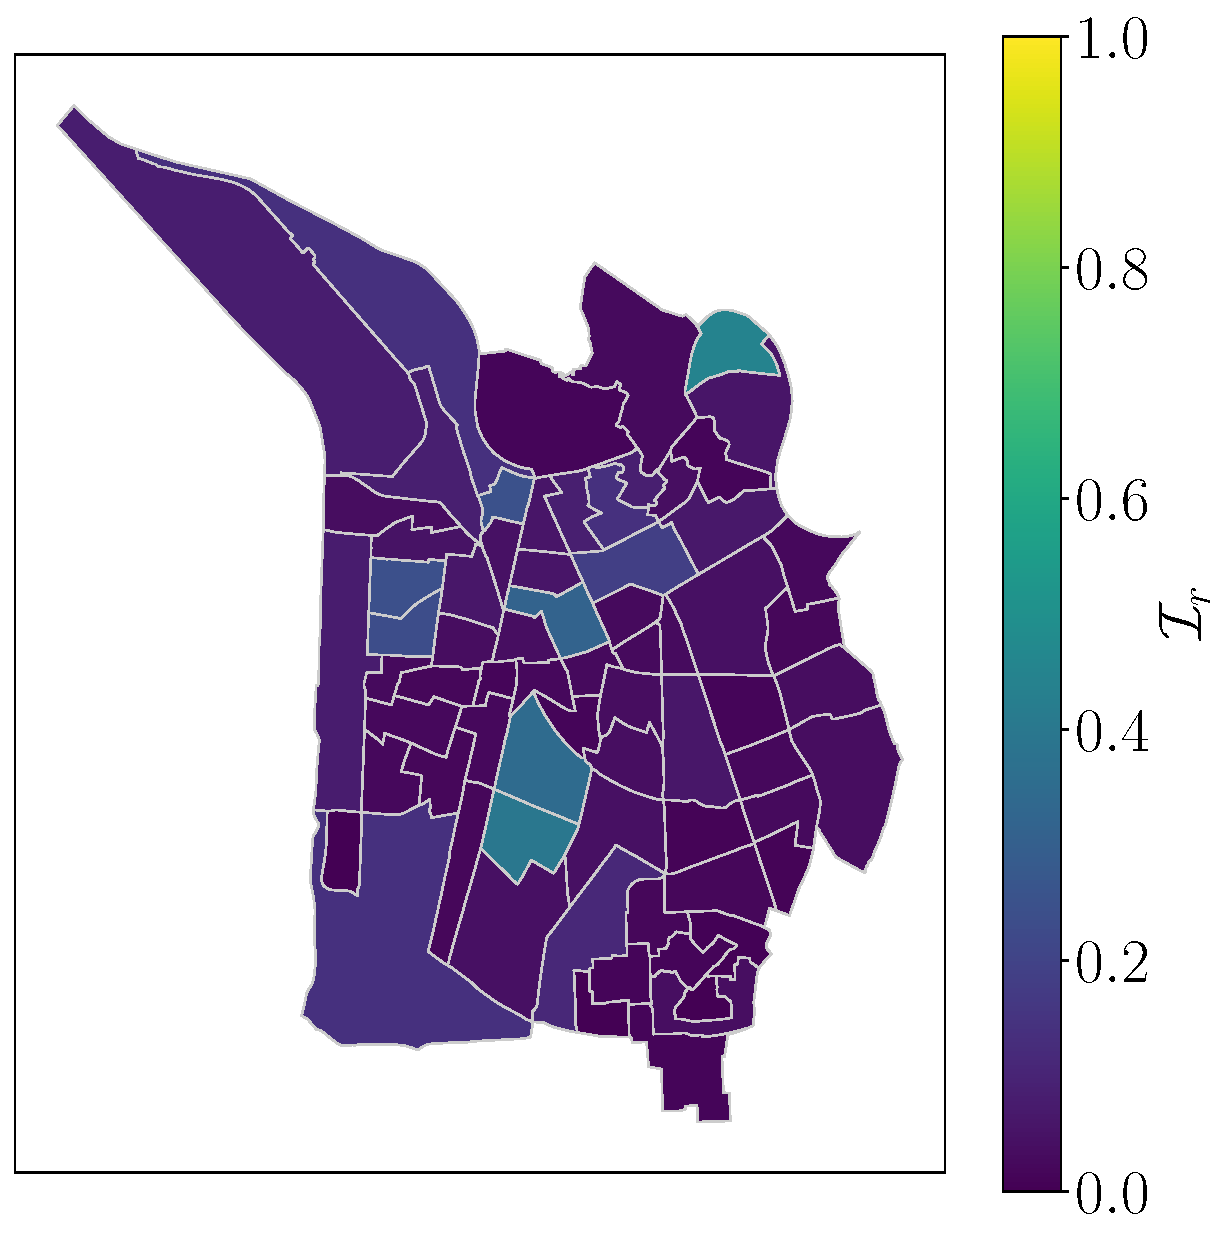
\includegraphics[width=0.24\linewidth]{Images/ut_regional_1_2.pdf}\label{2_3}}
  \hspace{0.004\linewidth}
  \subfloat[\mbox{Sufficientarian} safety path insufficiency]
  {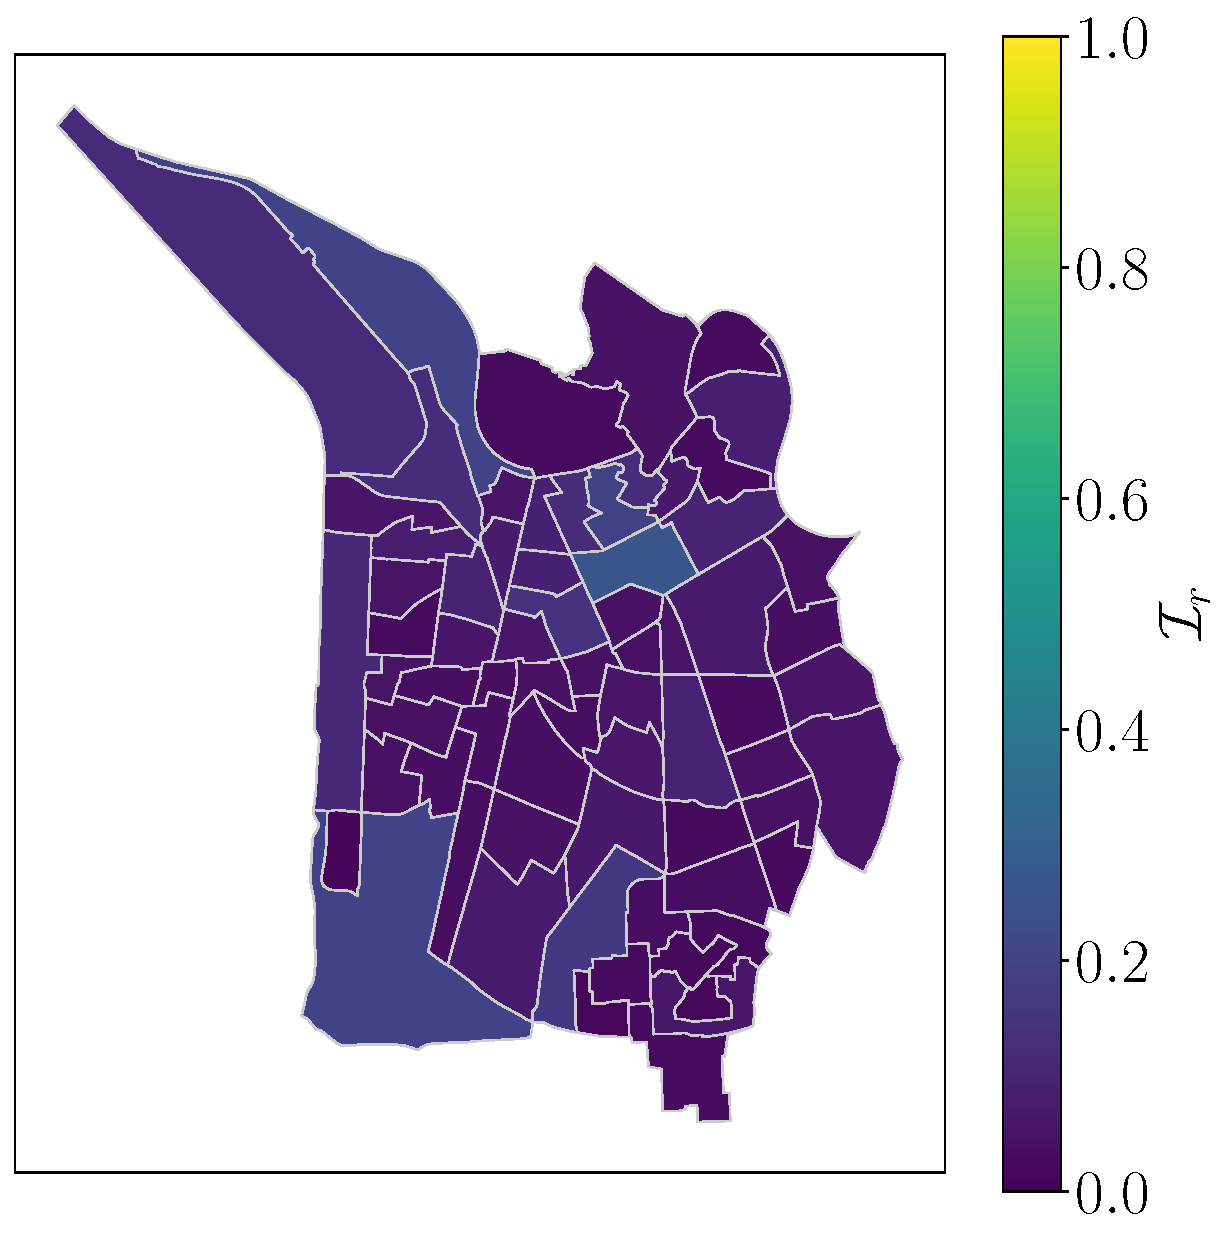
\includegraphics[width=0.24\linewidth]{Images/suff_regional_1_2.pdf}\label{2_4}}\\
  \subfloat[Original bike travel time insufficiency]{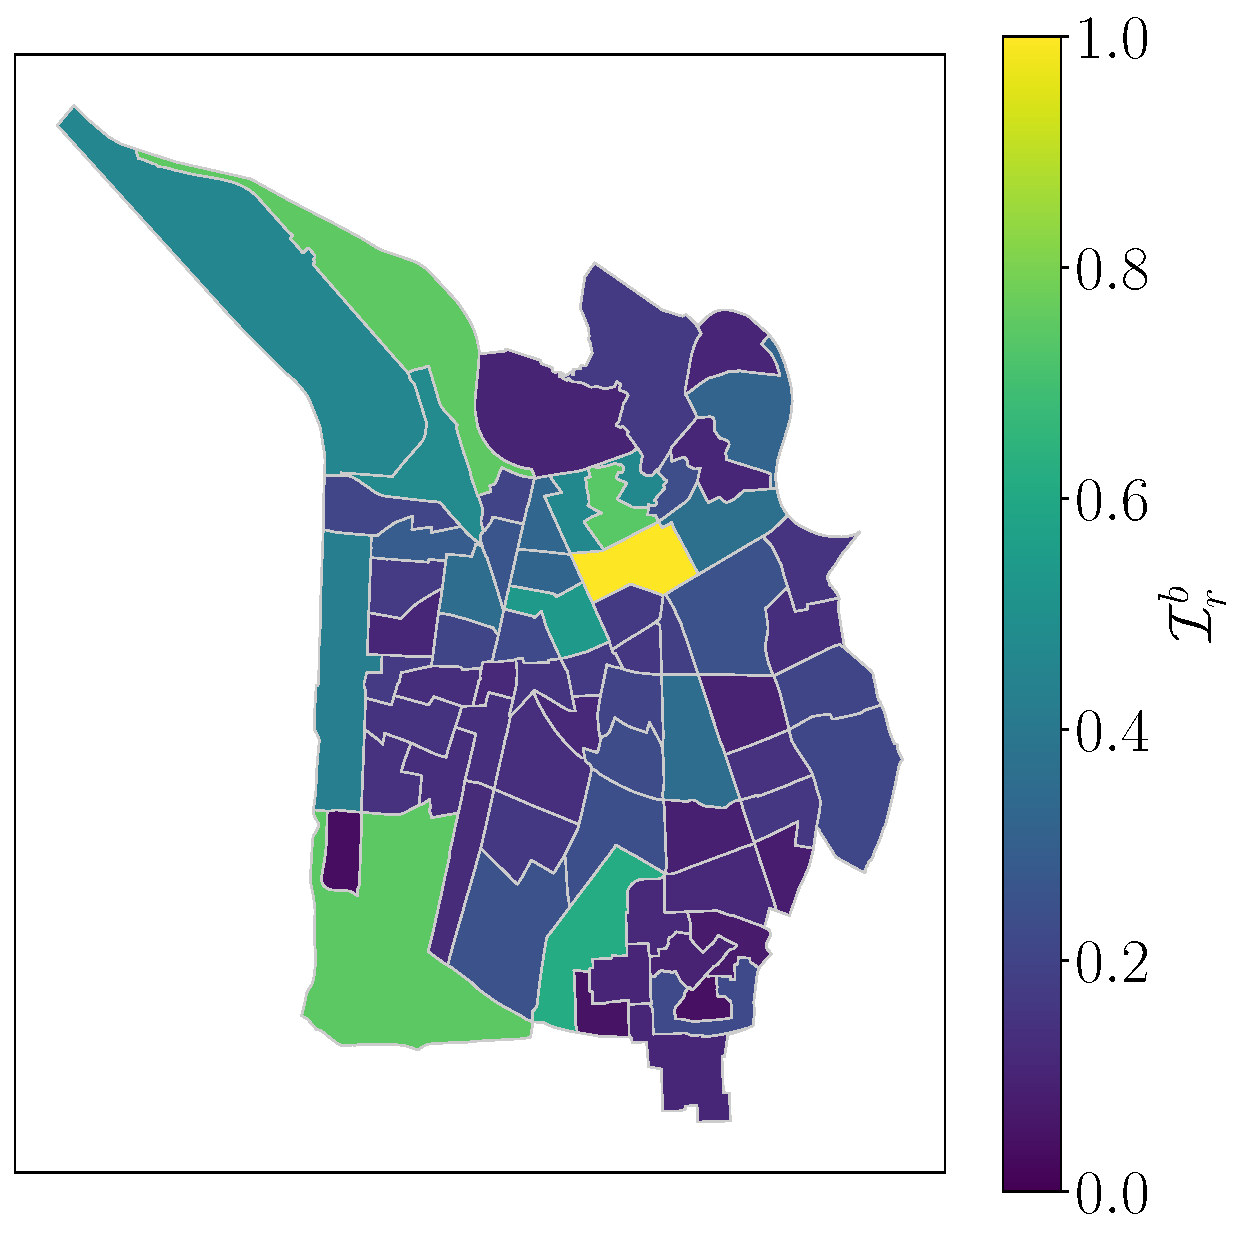
\includegraphics[width=0.24\linewidth]{Images/G_original_regional_bike_time_1_2.pdf}\label{3_1}}
  \hspace{0.004\linewidth} % Adjust horizontal space as 
  \subfloat[\mbox{Utilitarian} bike travel time insufficiency]
  {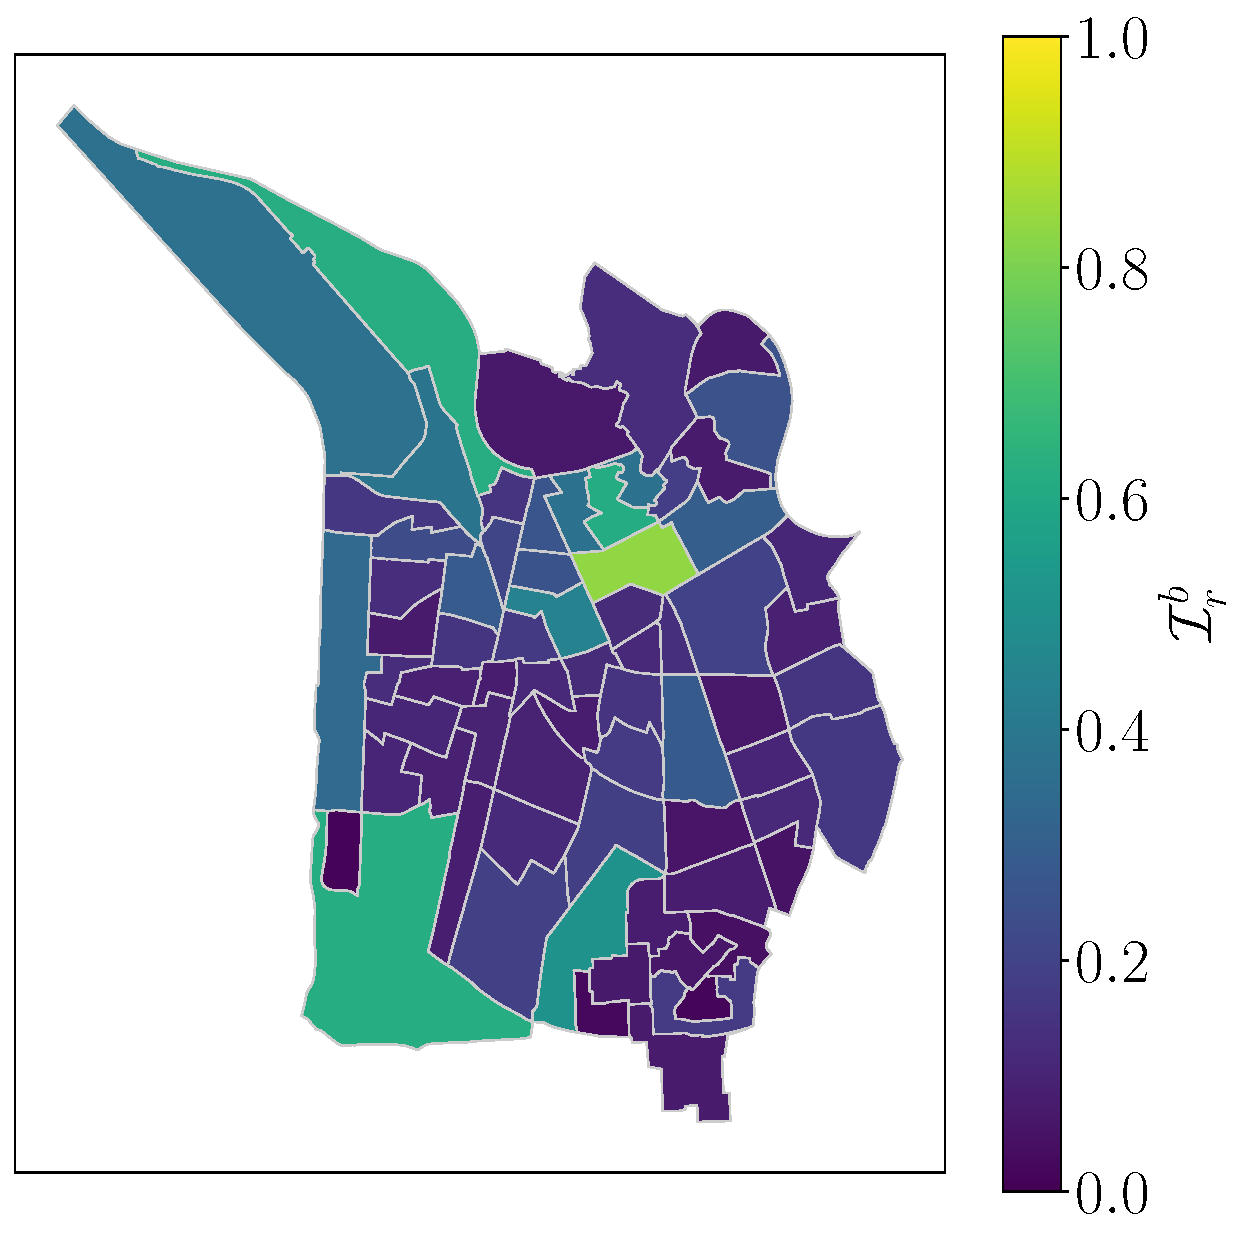
\includegraphics[width=0.24\linewidth]{Images/ut_regional_bike_time_1_2.pdf}\label{3_3}}
  \hspace{0.004\linewidth}
  \subfloat[\mbox{Sufficientarian} bike travel time insufficiency]
  {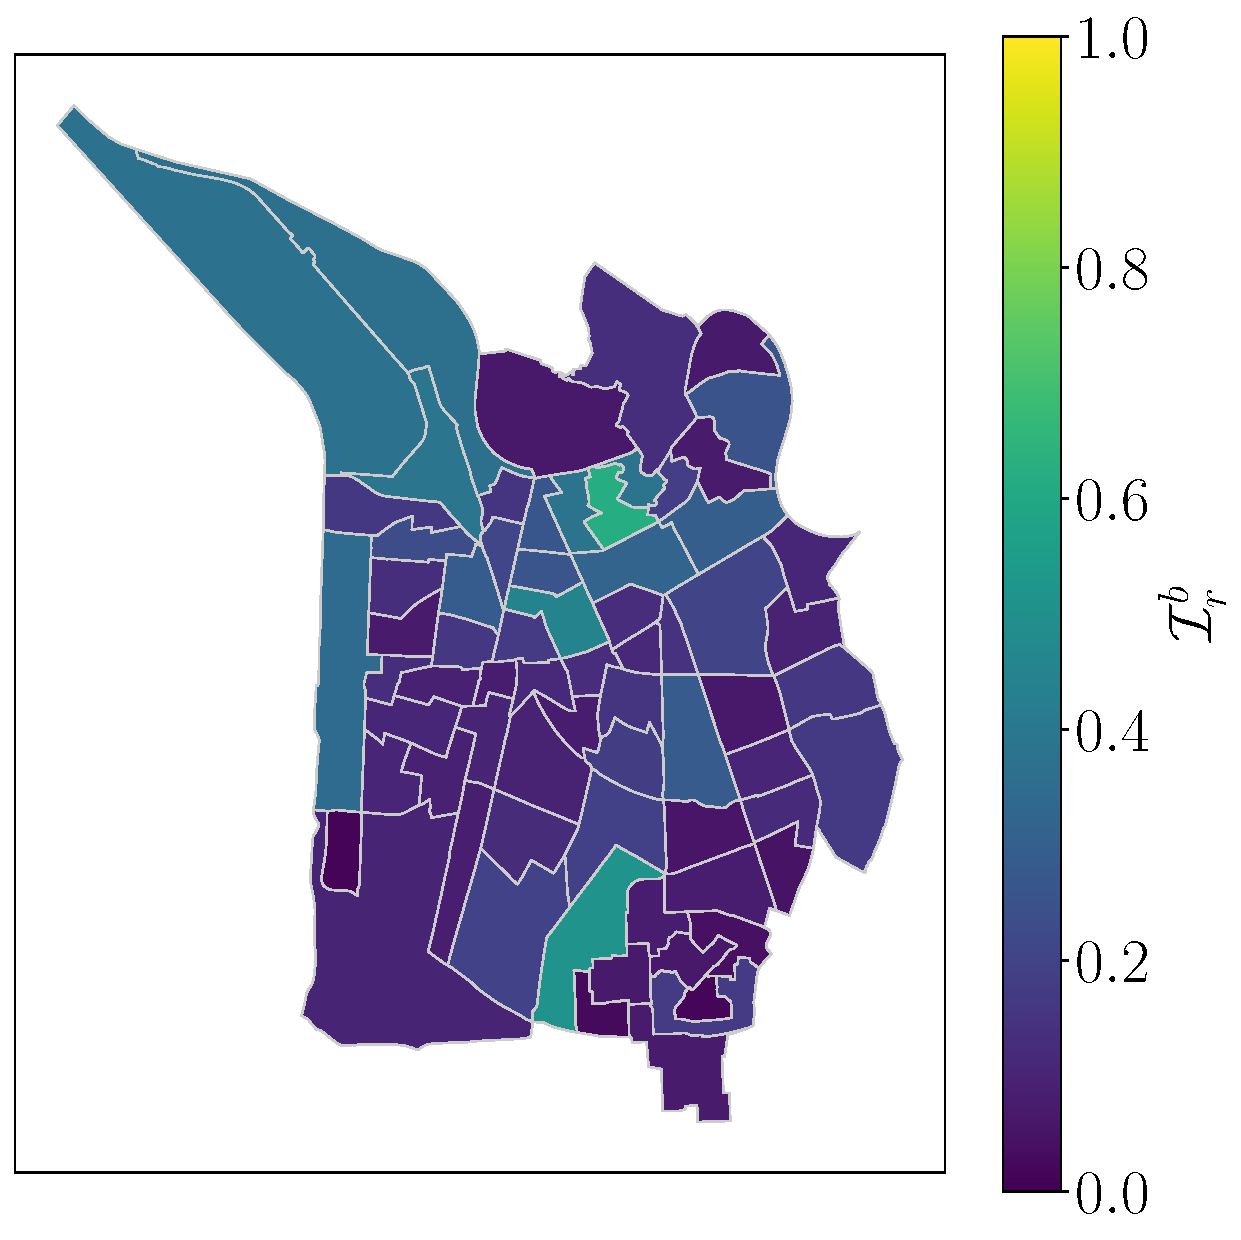
\includegraphics[width=0.24\linewidth]{Images/suff_regional_bike_time_1_2.pdf}\label{3_4}}
  \\
  \subfloat[Original car travel time insufficiency]{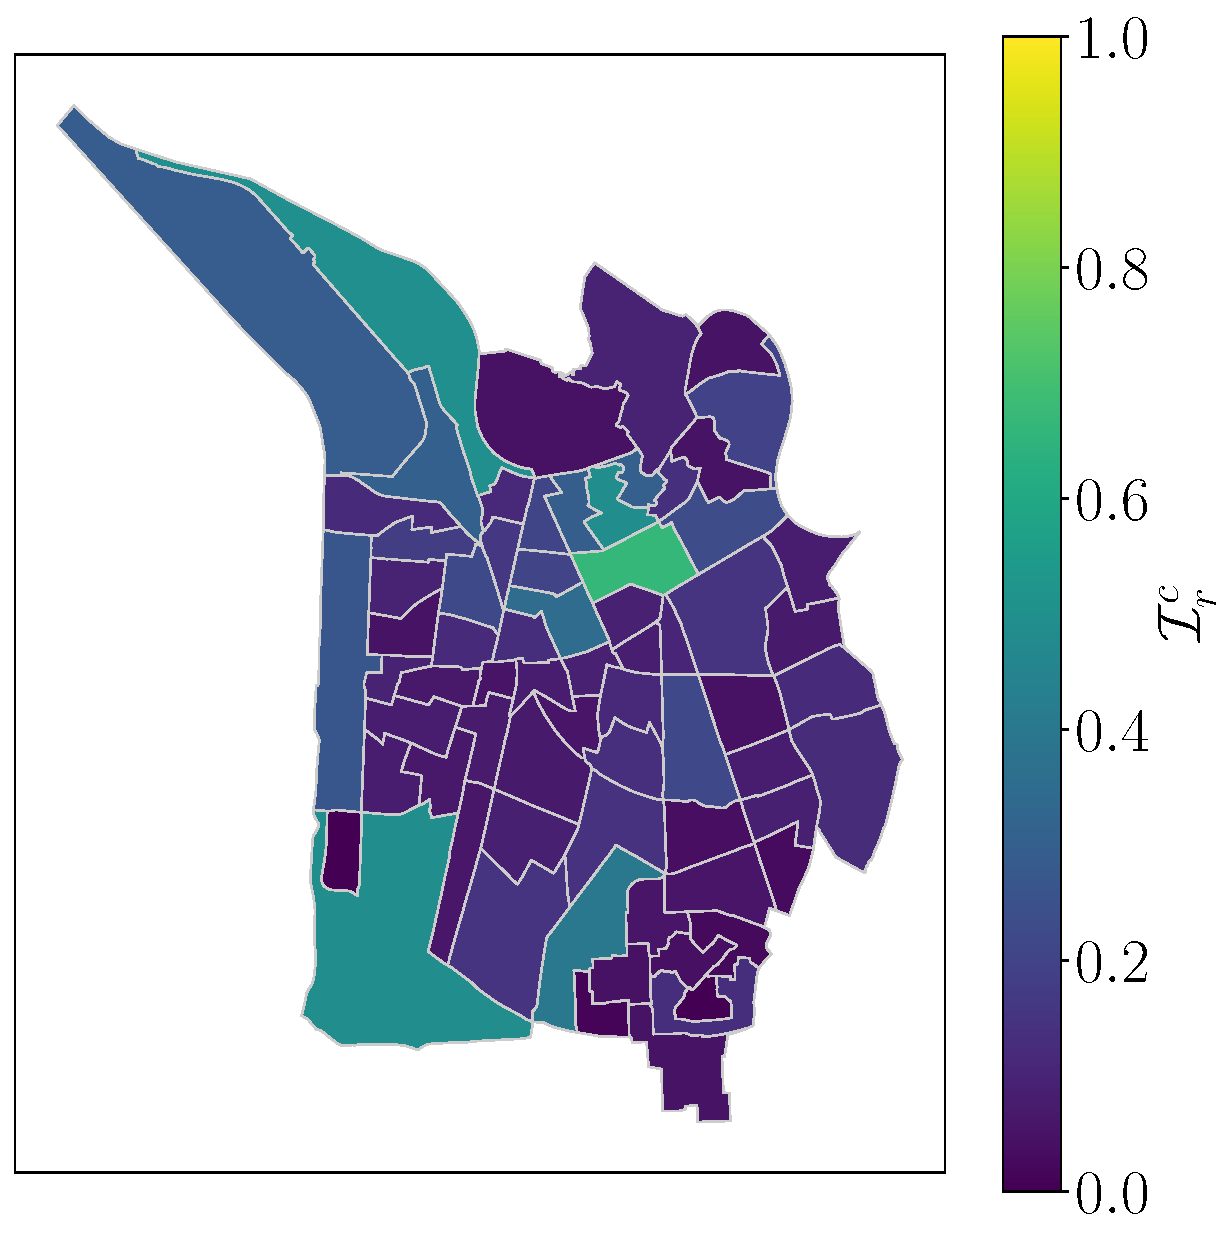
\includegraphics[width=0.24\linewidth]{Images/G_original_regional_car_time_1_2.pdf}\label{4_1}}
  \hspace{0.004\linewidth} % Adjust horizontal space as 
  \subfloat[\mbox{Utilitarian} car travel time insufficiency]
  {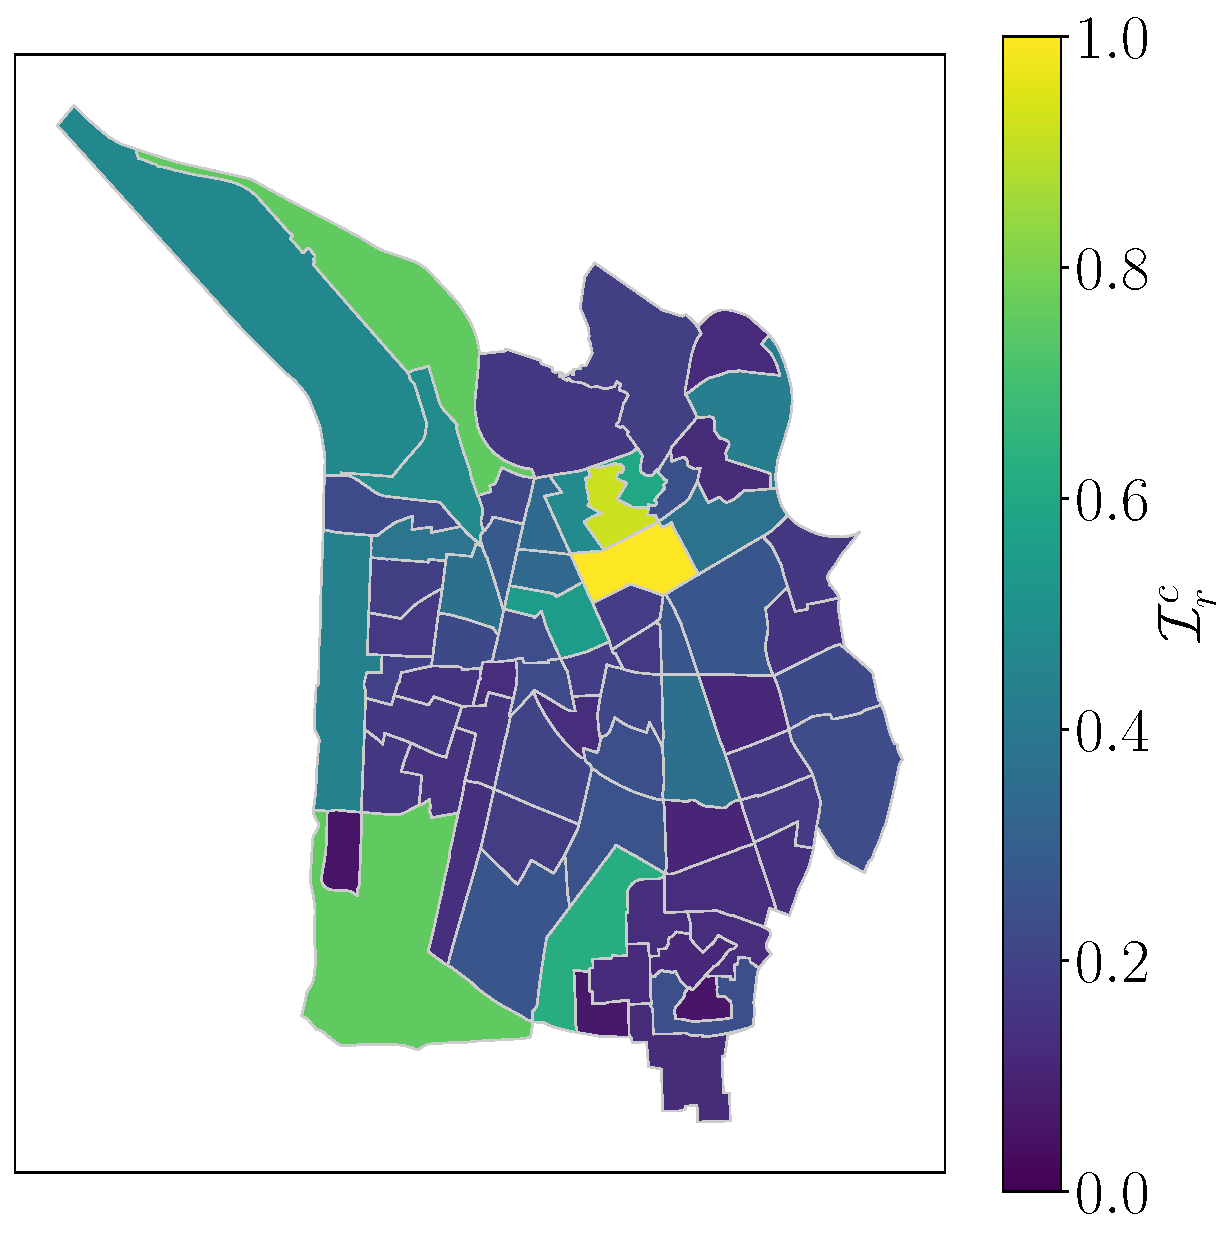
\includegraphics[width=0.24\linewidth]{Images/ut_regional_car_time_1_2.pdf}\label{4_3}}
  \hspace{0.004\linewidth}
  \subfloat[\mbox{Sufficientarian} car travel time insufficiency]
  {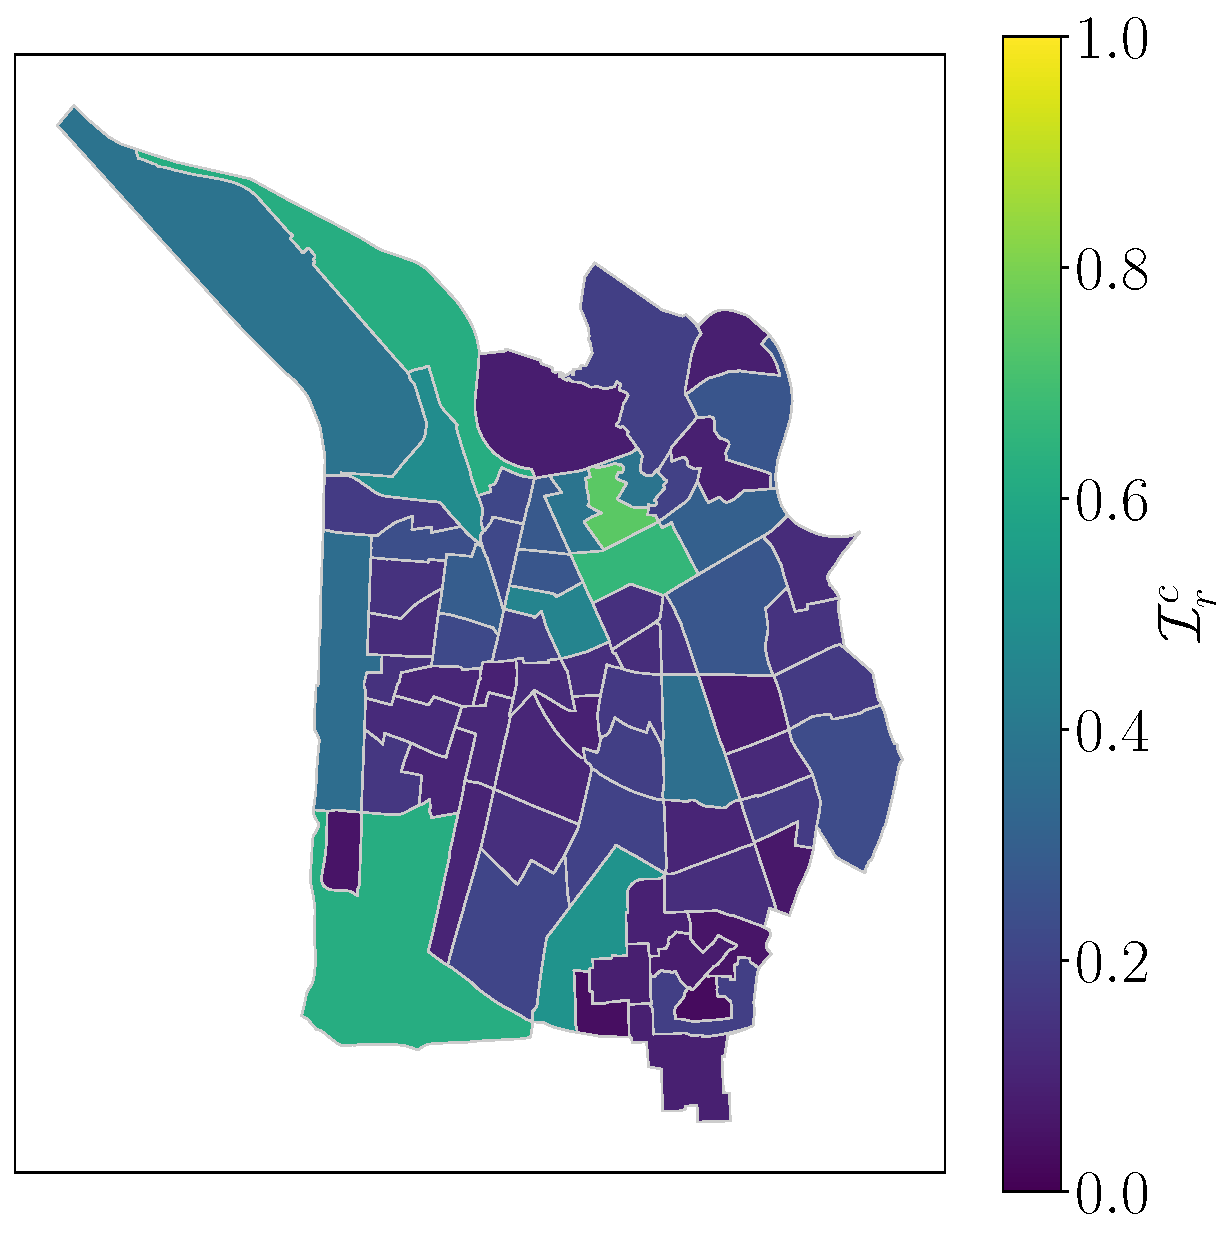
\includegraphics[width=0.24\linewidth]{Images/suff_regional_car_time_1_2.pdf}\label{4_4}}
   
  
  \caption{\footnotesize The top section reports the degree-of-separation (DoS) configurations together with their corresponding average cycling distance$\bar{D}^\mathrm{b}$ and bicycle mode share $P^\mathrm{b}$, while the bottom panels illustrate the regional exposure-based path insufficiency, bicycle travel time insufficiency, and car travel time insufficiency, respectively.  All optimization algorithms are applied with a exposure-based path insufficiency threshold of $\lambda = \mathrm{40 \%}$ and a budget of $B \approx 0.15\,B_{\max}$.
}
  \label{grenoble_dos}
\end{figure*}

% To illustrate these effects, Fig.~\ref{grenoble_dos} compares the original DoS distribution and regional exposure-based path insufficiency with the results obtained after applying the MLCC, \mbox{Utilitarian}, and \mbox{Sufficientarian} optimization strategies for $\lambda =40$\%.
% In Fig.~\ref{grenoble_dos}\textbf{(b)}, MLCC concentrates the entire budget on connecting regions with high path-exposure-based path insufficiency to the largest connected component with high DoS scores, prioritizing the safest available links. Conversely, \mbox{Utilitarian} (Fig.~\ref{grenoble_dos}\textbf{(c)}) distributes the investment more evenly across the network, balancing safety improvements throughout. Both \mbox{Sufficientarian} and \mbox{MLCC} achieve the greatest reductions in regional path-exposure-based path insufficiency (Fig.~\ref{grenoble_dos}\textbf{(i)}–\textbf{(l)}) while also mitigating bicycle accessibility unfairness. However, only \mbox{Sufficientarian} reduces the negative accessibility impact on cars following the lane upgrades (Fig.~\ref{grenoble_dos}\textbf{(m)}–\textbf{(p)}). In contrast, MLCC causes the greatest disruption to the car network, leading to higher driver accessibility unfairness due to the formation of a large connected component that forces longer detours. Fig.~\ref{histograms_plots} shows the relationship between path-safety scores and the number of cyclists for each method. Both MLCC and \mbox{Sufficientarian} result in a larger share of cyclists exceeding the exposure-based path-protection threshold. Fig.~\ref{histograms_plots_justice} presents an analogous analysis for both cyclists and drivers, showing the number of individuals above and below the trip-sufficiency threshold. While MLCC and \mbox{Utilitarian} both effectively reduce cyclist accessibility unfairness, only \mbox{Sufficientarian} enables more car drivers to remain below the time threshold, preventing a larger proportion of car users from exceeding it despite the reduced car-lane capacity associated with bike-lane upgrades. Fig.~\ref{Percentage_thr} illustrates, for $\lambda = \mathrm{40 \%}$, the percentage of cyclists above and below the exposure-based path-protection threshold. It can be observed that both MLCC and \mbox{Sufficientarian} achieve the greatest improvements in Exposure-based path-sufficiency score and cyclist travel time. However, only MLCC effectively mitigates the impact on car travel times, resulting in the lowest overall increase in travel time for motorized traffic.  

% To illustrate these effects, Fig.~\ref{histograms_plots} shows the relationship between path-safety scores and the number of cyclists for each method. Both MLCC and \mbox{Sufficientarian} lead to a larger share of cyclists exceeding the exposure-based path-protection threshold. Fig.~\ref{histograms_plots_justice} extends this analysis to both cyclists and drivers, showing the number of individuals above and below the trip-sufficiency threshold. While MLCC and \mbox{Utilitarian} effectively reduce cyclist accessibility unfairness, only \mbox{Sufficientarian} allows more car drivers to remain below the time threshold, minimizing travel-time excess despite the reduced car-lane capacity caused by bike-lane upgrades.
% Fig.~\ref{Percentage_thr} illustrates, for $\lambda = \mathrm{40 \%}$, the percentage of cyclists above and below the exposure-based path-protection threshold. Both MLCC and \mbox{Sufficientarian} improve Exposure-based path-sufficiency score and cyclist travel time; however, only MLCC mitigates the impact on car travel times, resulting in the lowest increase in travel time for motorized traffic.
% Finally, Fig.~\ref{grenoble_dos} compares the original DoS distribution and regional exposure-based path insufficiency before and after applying the MLCC, \mbox{Utilitarian}, and \mbox{Sufficientarian} optimization strategies ($\lambda = 40\%$). MLCC concentrates the budget on connecting high-insufficiency regions to the safest network components, while \mbox{Utilitarian} distributes investments more evenly. Both \mbox{Sufficientarian} and MLCC achieve the largest reductions in regional exposure-based path insufficiency and bicycle accessibility unfairness, but only \mbox{Sufficientarian} limits the negative accessibility impacts on cars.
% Fig.~\ref{unfairness_result} presents the results of the sufficientarian approach in Problem~2, specifically to calculate the upper level $\mathbb{U}_{\text{thr}}$ for the different candidate solutions and threshold values given by  $\lambda$. We observe that when $\lambda$ is small, exposure-based path insufficiency remains low. However, as $\lambda$ increases, insufficiency also rises. Despite this, MLCC and \mbox{Sufficientarian} repeatedly achieve the greatest reductions in exposure-based path insufficiency.

To illustrate these effects, Fig.~\ref{histograms_plots} reports the distribution of path-safety scores and the corresponding number of cyclists for each method. Overall, \mbox{the sufficientarian formulation} yields a larger share of cyclists traveling on routes that exceed the exposure-based path-protection threshold. Fig.~\ref{histograms_plots_justice} extends this analysis to both cyclists and drivers by showing the proportions of users above and below the trip-sufficiency threshold. While \mbox{the utilitarian formulation} reduces cyclist trip insufficiency, only \mbox{the sufficientarian formulation} keeps a larger share of drivers below the time threshold, thereby limiting travel-time exceedances despite the road-capacity reductions induced by bike-lane upgrades. Fig.~\ref{Percentage_thr} further summarizes, for $\lambda = \mathrm{40\%}$, the percentage of cyclists above and below the exposure-based path-protection threshold. In this setting, \mbox{the sufficientarian formulation} improves exposure-based path-sufficiency score while also maintaining comparatively low increases in car travel times, resulting in the smallest impact on motorized traffic. Finally, Fig.~\ref{grenoble_dos} compares the DoS distribution and the spatial pattern of regional exposure-based path insufficiency before and after solving the utilitarian and sufficientarian formulations ($\lambda = 40\%$). Whereas \mbox{the utilitarian formulation} tends to distribute investments more evenly, \mbox{the sufficientarian formulation} achieves the largest reductions in regional exposure-based path insufficiency and bicycle trip insufficiency, while also better limiting the negative trip-time impacts on drivers. Fig.~\ref{unfairness_result} presents the sufficientarian outcomes of Problem~2 by reporting the upper-level objective $\mathbb{U}_{\text{thr}}$ across candidate solutions and threshold values $\lambda$. When $\lambda$ is small, exposure-based path insufficiency remains low; as $\lambda$ increases, insufficiency rises. Across thresholds, \mbox{the sufficientarian formulation} consistently achieves the largest reductions in exposure-based path insufficiency.

%%%%%%%%%%%%%%%%%%%%%%%%%%%%%%%%%%%%%%%%%%%%%%%%%%%%%%%%%%%%%%


% To illustrate these effects, Fig.~\ref{histograms_plots} shows the relationship between path-safety scores and the number of cyclists for each method. Note that \mbox{the sufficientarian formulation} lead to a larger share of cyclists exceeding the exposure-based path-protection threshold. Fig.~\ref{histograms_plots_justice} extends this analysis to both cyclists and drivers, showing the number of individuals above and below the trip-sufficiency threshold. While \mbox{the utilitarian formulation} effectively reduces cyclist accessibility unfairness, only \mbox{the sufficientarian formulation} allows more car drivers to remain below the time threshold, minimizing travel-time excess despite the reduced car-lane capacity caused by bike-lane upgrades.
% Fig.~\ref{Percentage_thr} illustrates, for $\lambda = \mathrm{40 \%}$, the percentage of cyclists above and below the exposure-based path-protection threshold. We have that \mbox{the sufficientarian formulation} improves Exposure-based path-sufficiency score and cyclist travel time and mitigates the impact on car travel times, resulting in the lowest increase in travel time for motorized traffic.
% Finally, Fig.~\ref{grenoble_dos} compares the original DoS distribution and regional exposure-based path insufficiency before and after applying the \mbox{the utilitarian formulation}, and \mbox{the sufficientarian formulation} optimization strategies ($\lambda = 40\%$), while \mbox{the utilitarian formulation} distributes investments more evenly, \mbox{the sufficientarian formulation} achieves the largest reductions in regional exposure-based path insufficiency and bicycle accessibility unfairness, and only \mbox{the sufficientarian formulation} limits the negative accessibility impacts on cars.

% Fig.~\ref{unfairness_result} presents the results of the sufficientarian approach in Problem~2, specifically to calculate the upper level $\mathbb{U}_{\text{thr}}$ for the different candidate solutions and threshold values given by  $\lambda$. We observe that when $\lambda$ is small, exposure-based path insufficiency remains low. However, as $\lambda$ increases, insufficiency also rises. Despite this, \mbox{the sufficientarian formulation} repeatedly achieves the greatest reductions in exposure-based path insufficiency.


%%%%%%%%%%%%%%%%%%%%%%%%%%%%%%%%%%%%%%%%%%%%%%%%%%%%%%%%%%%%%%

\begin{figure}[h!]
\vspace{0.2cm}
\centering
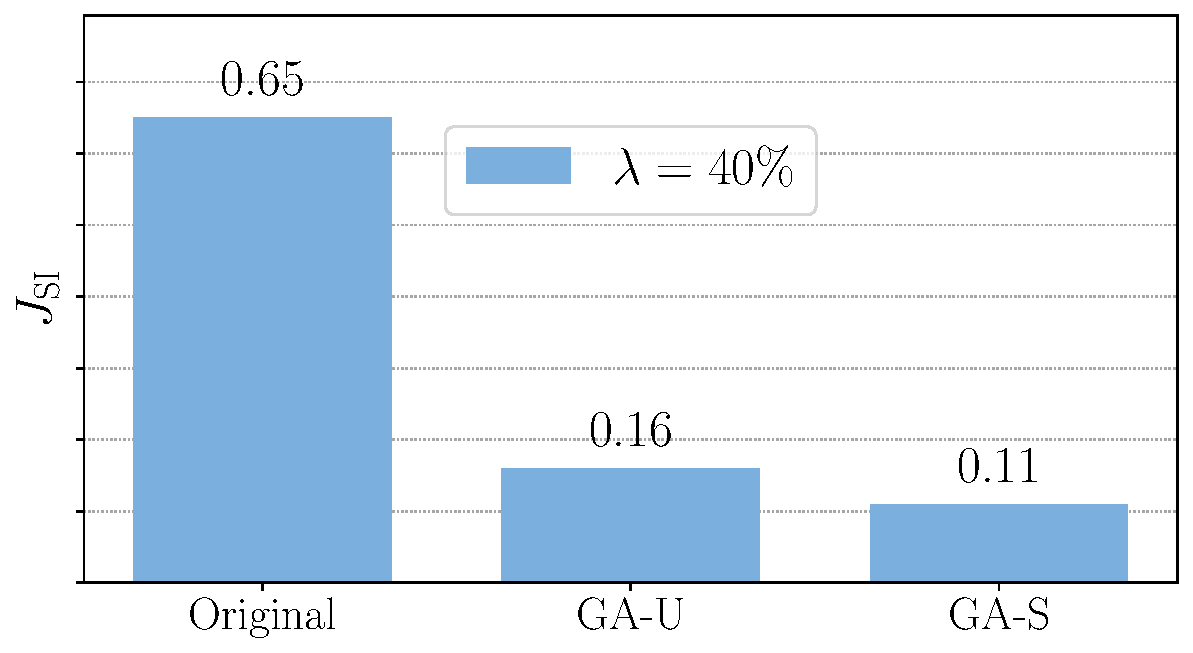
\includegraphics[width=\columnwidth]{Images/safety_insufficiency_reduction.pdf}
\caption{\footnotesize Exposure-based path insufficiency comparison of upper level $\mathbb{U}_{\text{thr}}$ of Problem~3, and the color legend indicates the $\lambda$ threshold.}
\label{unfairness_result}
\end{figure}

% \subsection{Total System Performance}
% To better interpret these findings, we compare them to a reference scenario in which exposure-based path insufficiency is not explicitly considered—namely, Problem~1, which focuses solely on minimizing cyclists’ exposure to motor traffic. 
% For this comparison, we examine the upper-level formulation $\mathbb{U}$.  As shown in the top panel of Fig.~\ref{cyclist_exposure_and_unfair}, \mbox{the utilitarian formulation} achieves the largest overall reduction in cyclist exposure, followed by MLCC. 
% Nevertheless, \mbox{the sufficientarian formulation} attains comparable performance across the evaluated thresholds, despite being designed to balance exposure-based path insufficiency and exposure reduction. 
% Because genetic algorithms typically yield locally optimal rather than globally optimal solutions, small variations may occur across problem instances. 
% However, the similar outcomes achieved by \mbox{the sufficientarian formulation} suggest that incorporating exposure-based path insufficiency considerations can improve overall network safety without substantially compromising exposure reduction. 
% To assess whether the proposed framework improves the overall travel efficiency of the system, 
% we evaluate the demand weighted total system travel time (TSTT) under an optimized cycling configuration 
% $\tilde{\boldsymbol{w}}^\mathrm{b}$. 
% The TSTT quantifies the aggregate temporal performance of the multi-modal network and is defined as the sum of the bicycle and car components:
% \begin{equation}
% \label{eq:sttt_def}
% \mathcal{TSTT}(\tilde{\boldsymbol{w}}^\mathrm{b})
% \;=\;
% \mathcal{TSTT}^\mathrm{b}(\tilde{\boldsymbol{w}}^\mathrm{b})
% \;+\;
% \tilde{\mathcal{TSTT}}^\mathrm{c}(\tilde{\boldsymbol{w}}^\mathrm{b}).
% \end{equation}
% The bicycle component, $\mathcal{TSTT}^\mathrm{b}$, corresponds to the demand-weighted aggregate travel time across all origin–destination (OD) pairs:
% \begin{equation}
% \label{eq:bike_ttt_weighted}
% \mathcal{TSTT}^\mathrm{b}(\tilde{\boldsymbol{w}}^\mathrm{b})
% \;=\;
% \sum_{(u,v) \in \mathcal{V} \times \mathcal{V}}
% q^\mathrm{b}_{(u,v)}(\tilde{\boldsymbol{w}}^\mathrm{b})\,
% T^\mathrm{b}_{p_{(u,v)}}(\tilde{\boldsymbol{w}}^\mathrm{b}),
% \end{equation}
% where $q^\mathrm{b}_{(u,v)}$ is the bicycle demand between nodes $u$ and $v$, and 
% $T^\mathrm{b}_{p_{(u,v)}}$ denotes the travel time along the corresponding path $p_{(u,v)}$. 
% Similarly, the car component is given by:
% \begin{equation}
% \label{eq:car_ttt_weighted}
% \tilde{\mathcal{TSTT}}^\mathrm{c}(\tilde{\boldsymbol{w}}^\mathrm{b})
% \;=\;
% \sum_{(u,v)\in \mathcal{V} \times \mathcal{V}}
% q^\mathrm{c}_{(u,v)}(\tilde{\boldsymbol{w}}^\mathrm{b})\,
% \tilde{T}^\mathrm{c}_{p_{(u,v)}}(\tilde{\boldsymbol{w}}^\mathrm{b}),
% \end{equation}
% where $\tilde{T}^\mathrm{c}_{p_{(u,v)}}$ represents the approximated car travel time predicted by the surrogate GCN model. 
% The tilde notation in $\tilde{\mathcal{TSTT}}^\mathrm{c}$ emphasizes that this quantity is derived from near-equilibrium flow predictions, 
% rather than from an explicitly computed user-equilibrium solution.
% Fig.~\ref{time_demand} presents the total system travel time $\mathcal{TSTT}(\tilde{\boldsymbol{w}}^\mathrm{b})$ across all configurations. 
% In every optimization scenario, the TSTT is reduced compared to the baseline, 
% primarily due to the modal shift from cars to bicycles. 
% This reduction reflects that cyclists reach their destinations more efficiently within safer and more comfortable networks. 
% Among the evaluated methods, the sufficientarian approach achieves the greatest decrease in demand weighted total system travel time, 
% indicating that incorporating a fairness-oriented perspective can simultaneously improve overall safety and reduce unfairness. 
% Finally, Fig.~\ref{grenoble_paths} illustrates representative cyclist and driver paths for the different configurations, 
% showing that only the sufficientarian framework enables both cyclists and drivers to remain below the time threshold. 
% These results suggest that a carefully designed sufficientarian strategy can enhance not only fairness but also 
% the overall temporal performance of the transport system, here represented by the two main travel modes—drivers and cyclists.

% This completely aligns with studies show that car drivers
% who correct their inaccurate knowledge of travel time with
% public transport and bike are more likely to use it in the future or at least consider in their choice set \cite{mitra2017mode, sharples2017travel, van2009could}. therefore, it is
% important to understand that using low-carbon modes can
% sometimes have comparable travel time to driving car, i.e.,
% there is a potential for time-relevant low-carbon transportation.
% \subsection{Total System Performance}
% To better interpret these findings, we compare them to a reference scenario in which exposure-based path insufficiency is not explicitly considered namely, Problem~2, which focuses solely on minimizing cyclists’ exposure to motor traffic. As shown in the top panel of Fig.~\ref{cyclist_exposure_and_unfair}, \mbox{the utilitarian formulation} achieves the largest overall reduction in cyclist exposure. Nevertheless, \mbox{the sufficientarian formulation} attains comparable performance across the evaluated thresholds, despite being designed to balance exposure-based path insufficiency and exposure reduction.

% To assess whether the proposed framework also improves the overall efficiency of the multi-modal system, we evaluate the total system travel time already defined in Eq.~\eqref{total_system_travel},
% \begin{equation}
%     \mathcal{T}_{\mathrm{tot}}(\boldsymbol{w}^\mathrm{b})
% =
% \mathcal{T}_\mathrm{b}(\boldsymbol{w}^\mathrm{b})
% +
% \mathcal{T}_\mathrm{c}(\boldsymbol{w}^\mathrm{b}).
% \end{equation}
% In the results reported below, $\mathcal{T}_{\mathrm{tot}}$ is interpreted as a demand-weighted system metric: the bicycle component aggregates OD travel times weighted by bicycle demand, while the car component aggregates link/path travel times weighted by car flows (or OD demand when using the surrogate predictor). This weighting ensures that the metric reflects the travel-time experienced by users, rather than treating every OD pair equally. Fig.~\ref{time_demand} shows that $\mathcal{T}_{\mathrm{tot}}(\boldsymbol{w}^\mathrm{b})$ decreases across all optimized configurations relative to the baseline, largely driven by the modal shift from cars to bicycles. Among the evaluated methods, the sufficientarian approach yields the largest reduction in $\mathcal{T}_{\mathrm{tot}}$, suggesting that incorporating a fairness-oriented perspective can simultaneously improve safety outcomes while maintaining (or improving) overall system efficiency.


%%%%%%%%%%%%%%%%%%%%%%%%%%%%%%%%%%%%%%%%%%%%%
% \subsection{Total System Performance}
% To better interpret these findings, we compare them to a reference scenario in which safety-path insufficiency is not explicitly considered, namely Problem~2, which focuses solely on minimizing cyclists' exposure to motor traffic. As shown in the top panel of Fig.~\ref{cyclist_exposure_and_unfair}, \mbox{the utilitarian formulation} achieves the largest overall reduction in cyclist exposure. Nevertheless, \mbox{the sufficientarian formulation} attains comparable exposure reductions across the evaluated thresholds, despite being designed to balance safety-path insufficiency and exposure.

% To assess whether the proposed framework also improves the overall efficiency of the multi-modal system, we evaluate the total system travel time defined in Eq.~\eqref{total_system_travel},
% \begin{equation}
% \mathcal{T}_{\mathrm{tot}}(\boldsymbol{w}^\mathrm{b})
% =
% \mathcal{T}_\mathrm{b}(\boldsymbol{w}^\mathrm{b})
% +
% \mathcal{T}_\mathrm{c}(\boldsymbol{w}^\mathrm{b}).
% \end{equation}
% In the results reported below, $\mathcal{T}_{\mathrm{tot}}$ is a demand-weighted time metric: the bicycle component aggregates OD travel times weighted by bicycle demand, while the car component aggregates link/path travel times weighted by car flows (or OD demand when using the surrogate predictor). Note that the total number of trips is fixed; only their allocation across modes changes through the mode-shift model.

% Fig.~\ref{time_demand} shows that, in the Grenoble case study, $\mathcal{T}_{\mathrm{tot}}(\boldsymbol{w}^\mathrm{b})$ is reduced for all optimized configurations relative to the baseline, which is consistent with a modal shift away from cars and the associated reduction in car congestion. Among the evaluated methods, the sufficientarian perspective yields the largest reduction in $\mathcal{T}_{\mathrm{tot}}$, suggesting that incorporating a fairness-oriented perspective can improve safety outcomes while maintaining (and in this case improving) overall system efficiency.

\subsection{Total System Performance}
To better interpret these findings, we compare them to a reference scenario in which safety-path insufficiency is not explicitly considered, namely Problem~2, which focuses solely on minimizing cyclists' exposure to motor traffic. As shown in the top panel of Fig.~\ref{cyclist_exposure_and_unfair}, \mbox{the utilitarian formulation} achieves the largest overall reduction in cyclist exposure. Nevertheless, \mbox{the sufficientarian formulation} attains comparable exposure reductions across the evaluated thresholds, despite being designed to balance safety-path insufficiency and exposure.

To assess whether the proposed framework also improves the overall efficiency of the multi-modal system, we evaluate the total system travel time defined in Eq.~\eqref{total_system_travel},
\begin{equation}
\mathcal{T}_{\mathrm{tot}}(\boldsymbol{w}^\mathrm{b})
=
\mathcal{T}_\mathrm{b}(\boldsymbol{w}^\mathrm{b})
+
\mathcal{T}_\mathrm{c}(\boldsymbol{w}^\mathrm{b}).
\end{equation}
In the results reported below, $\mathcal{T}_{\mathrm{tot}}$ is a demand-weighted time metric: the bicycle component aggregates OD travel times weighted by bicycle demand, while the car component aggregates link/path travel times weighted by car flows (or OD demand when using the surrogate predictor). The accompanying modal-share curves report how trips are reallocated across modes through the mode-shift model.

Fig.~\ref{time_demand} shows that, in the Grenoble case study, $\mathcal{T}_{\mathrm{tot}}(\boldsymbol{w}^\mathrm{b})$ decreases for all optimized configurations relative to the baseline (from $463.7$ to $437.5$ and $432.8$ thousand hours), consistent with a shift away from cars and the resulting reduction in car travel time. Among the evaluated methods, the sufficientarian perspective yields the largest reduction in $\mathcal{T}_{\mathrm{tot}}$, suggesting that a sufficientarian perspective can improve safety outcomes while maintaining (and here improving) overall system efficiency.

%%%%%%%%%%%%%%%%%%%%%%%%%%%%%%%%%%%%%%%%%%%%%



\begin{figure}[t]
\vspace{0.2cm}
  \centering
  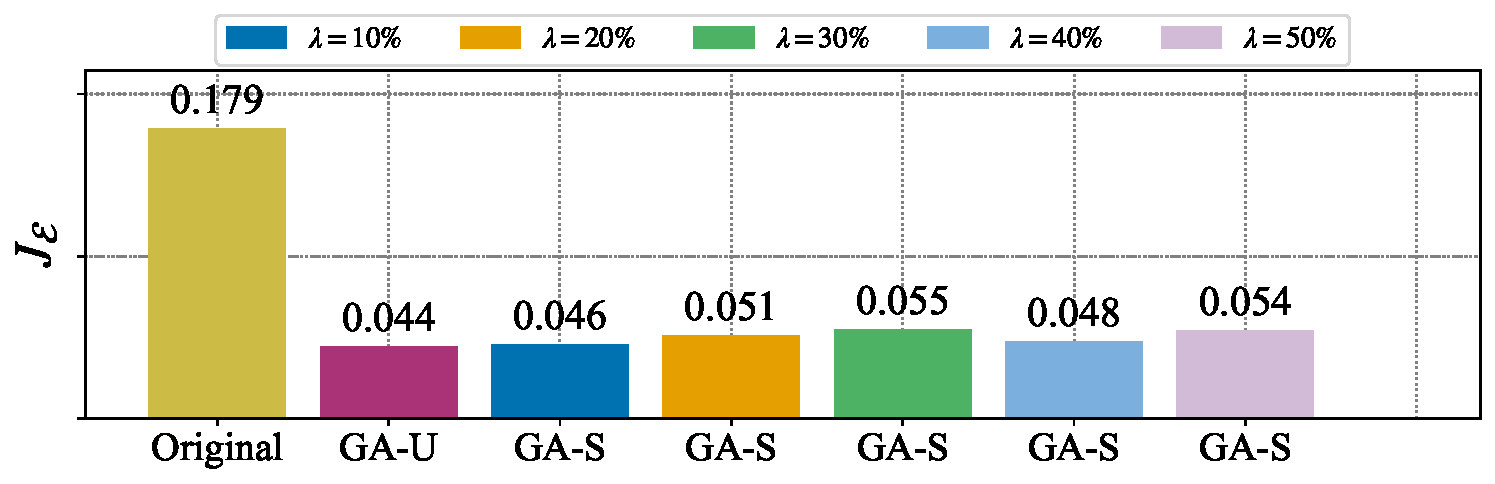
\includegraphics[width=1\linewidth]{Images/cyclist_exposure.pdf}

  
  \caption{On the top normalized cyclist exposure.}
  \label{cyclist_exposure_and_unfair}
\end{figure}

\begin{figure}[t]
\vspace{0.2cm}
  \centering
  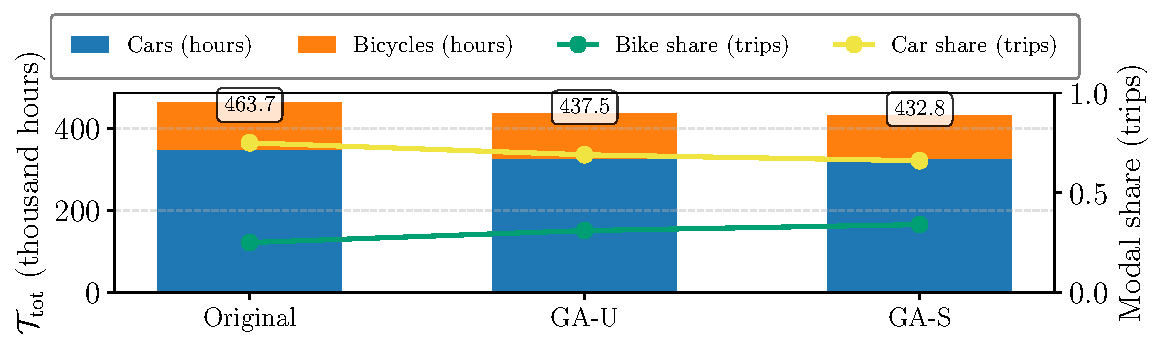
\includegraphics[width=1\linewidth]{Images/time_demand_comparison.pdf}

  
  \caption{Total system travel time ($\mathcal{T}_{\mathrm{tot}}$).}
  \label{time_demand}
\end{figure}

\begin{figure*}[t]
\vspace{0.2cm}
  \centering
  \captionsetup[subfigure]{font={footnotesize}, labelfont={footnotesize, bf}, textfont={footnotesize, rm}}

  \subfloat[Original DoS]{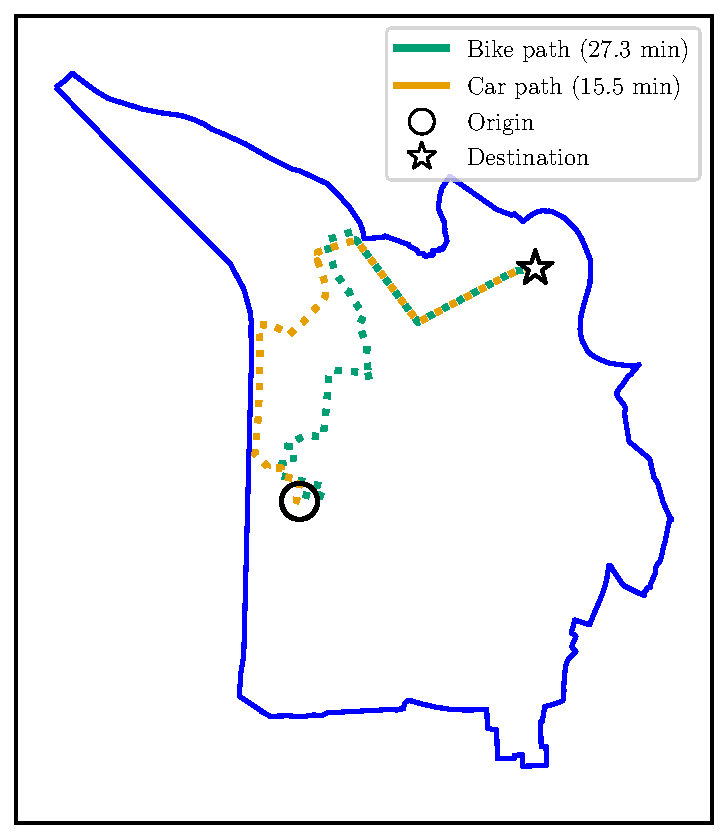
\includegraphics[width=0.25\linewidth]{Images/shortest_paths_bike_vs_car_original.pdf}\label{p_1}}
  \hspace{0.012\linewidth} % Adjust horizontal space as 
  % \subfloat[MLCC DoS]
  % {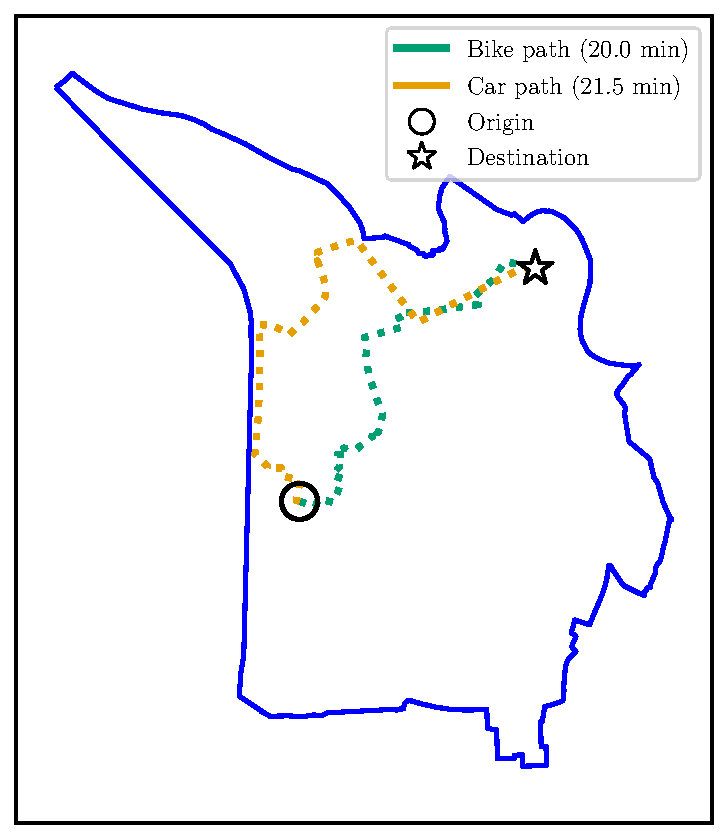
\includegraphics[width=0.23\linewidth]{Images/shortest_paths_bike_vs_car_MLCC.pdf}\label{p_2}}
  % \hspace{0.012\linewidth}
  \subfloat[\mbox{utilitarian} DoS]
  {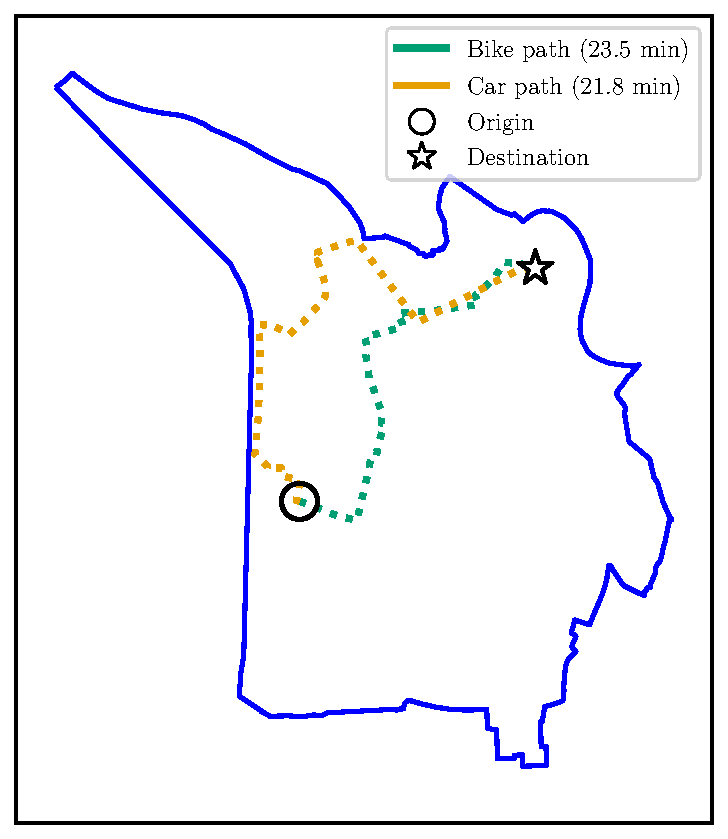
\includegraphics[width=0.25\linewidth]{Images/shortest_paths_bike_vs_car_utu.pdf}\label{p_3}}
  \hspace{0.012\linewidth}
  \subfloat[\mbox{Sufficientarian} DoS]
  {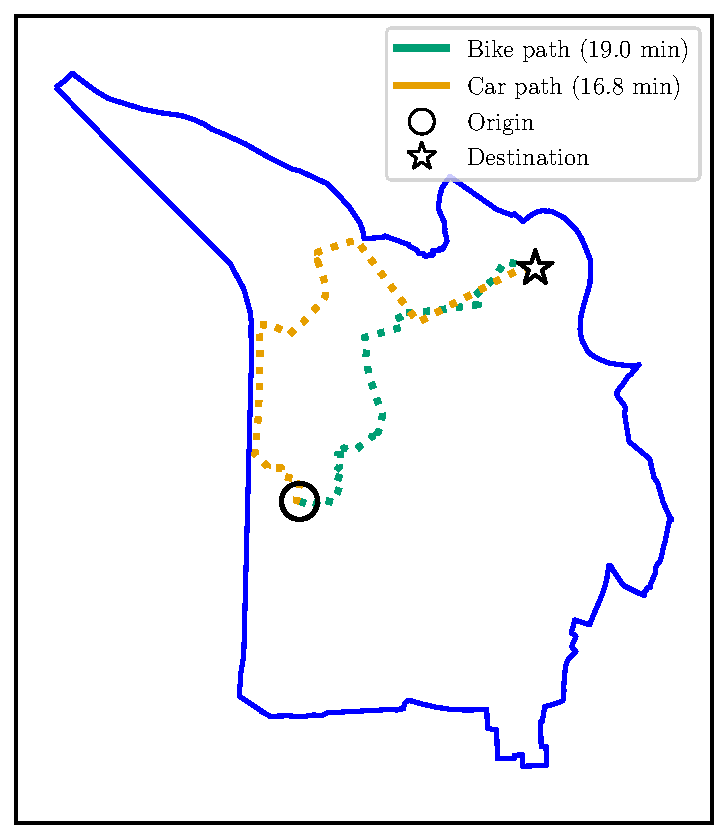
\includegraphics[width=0.25\linewidth]{Images/shortest_paths_bike_vs_car_suff.pdf}\label{p_4}}
   
  
  \caption{\footnotesize Grenoble configuration paths under different optimizations algorithms.}
  \label{grenoble_paths}
\end{figure*}

\section{Conclusion and Future Work}
% This work introduced a multi-modal bi-level optimization framework that integrates transport justice perspectives, mode-shift modeling, and multi-modal traffic assignment to support cycling infrastructure planning. Applied to the Grenoble network, the main lesson is that justice-oriented network upgrades can substantially improve cyclist safety and accessibility fairness \emph{without compromising efficiency}: safety outcomes (cyclist exposure and safety-path insufficiency) can be improved while keeping total system travel time impacts limited. Across the tested approaches, the sufficientarian perspective (Sufficientarian) provided the most balanced trade-off, reducing both cyclist and driver trip insufficiency while maintaining overall system performance.

% Future work will extend the mode-shift component by integrating additional social and behavioral determinants beyond infrastructure (e.g., city investments, policy incentives, and historical context) to better reflect real-world travel behavior \cite{glachant2024negotiating}. The framework will also be validated across several French cities to assess robustness across different network structures and to strengthen its policy relevance.
This work introduced a multi-modal bi-level optimization framework that combines transport justice, modal-shift modeling, and traffic assignment for cycling infrastructure planning. Applied to the Grenoble network, the results show that cycling infrastructure upgrades can reduce cyclist exposure and exposure-based path insufficiency while keeping increases in total system travel time limited for the tested budget and parameter settings. The comparison between utilitarian and sufficientarian formulations illustrates how different justice principles lead to different infrastructure priorities: the utilitarian formulation emphasizes aggregate exposure and travel-time performance, whereas the sufficientarian formulation more directly targets users experiencing inadequate exposure-based path protection or excessive trip travel times. Among the tested configurations, the sufficientarian genetic algorithm provides the most balanced outcome, reducing exposure-based path and trip insufficiency while maintaining competitive overall performance. However, these conclusions are based on selected values of the trade-off and sufficiency parameters, chosen to illustrate representative outcomes; future work will extend the mode-shift component by integrating additional social and behavioral determinants beyond infrastructure (e.g., city investments, policy incentives, and historical context) to better reflect real-world travel behavior \cite{glachant2024negotiating}. The framework will also be validated across several cities to assess robustness across different network structures and to strengthen its policy relevance.


\section*{Acknowledgment}
We thank Dr. I. New for proofreading this paper and
for re-humanizing sections where LLMs had been used to
improve grammar and flow. All resulting text was reviewed and revised by the authors.



\bibliographystyle{unsrt}
\bibliography{mybibfile}


\begin{IEEEbiography}[{
\includegraphics[width=1in,height=1.25in,clip,keepaspectratio]{Images/MCJ.pdf}}]{Manuel Campero Jurado}
Manuel Campero Jurado received the B.S. degree in applied mathematics in 2019 and the M.S. degree in mathematics in 2021, both from the Autonomous University of the State of Hidalgo, Mexico, and the Ph.D. degree from the Grenoble Institute of Technology, Grenoble, France in 2026. He is currently a postdoctoral researcher at IFP Energies nouvelles (IFPEN), Rueil-Malmaison, France. His research interests include modeling and optimization of transport networks, with a focus on low-carbon mobility.
\end{IEEEbiography}
\vspace{-1cm}
\begin{IEEEbiography}[{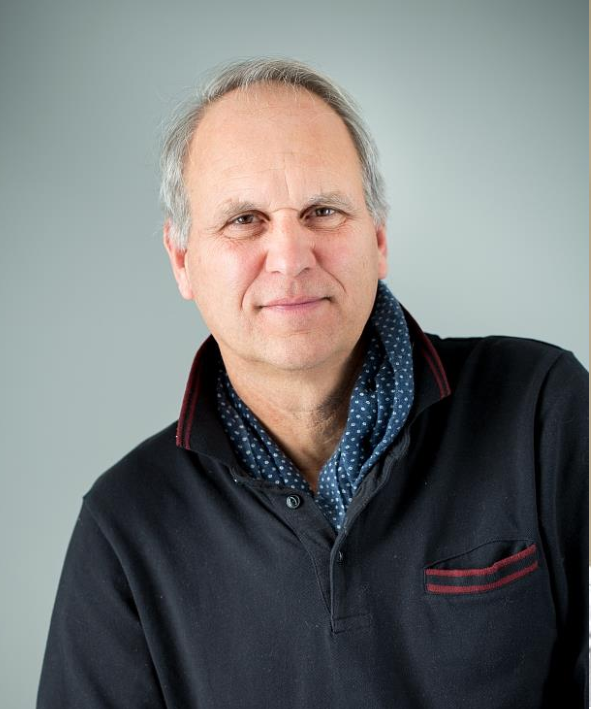
\includegraphics[width=1in,height=1.25in,clip,keepaspectratio]{Images/CCDW.pdf}}]{Carlos Canudas de Wit}
 received the B.Sc. degree in electronics and communications from the Monterrey Institute of Technology, Mexico, in 1980, and the M.Sc. and Ph.D. degrees in automatic control from the Grenoble Institute of Technology, France, in 1984 and 1987, respectively. He is a Directeur de recherche (Senior Researcher) at CNRS, Grenoble, where he leads the NeCS team (GIPSA-Lab and INRIA) on networked controlled systems. He is an IFAC Fellow, has served as Associate Editor for several IEEE journals, and was President of the European Control Association from 2013 to 2015. He held the ERC Advanced Grant Scale-FreeBack from 2016 to 2021. His research focuses on electric vehicles, optimal control, traffic modeling, and large-scale networks.
\end{IEEEbiography}
\vspace{-2cm}
\begin{IEEEbiography}[{
\includegraphics[width=1in,height=1.25in,clip,keepaspectratio]{Images/GDN.pdf}}]{Giovanni De Nunzio}
received his B.Sc. and M.Sc. degrees in Information and Automation Engineering from the University of L’Aquila, Italy, in 2007 and 2010, respectively, and the Ph.D. degree in Automatic Control from the Grenoble Institute of Technology (Grenoble INP), France, in 2015. He is currently a Research Engineer and a Research and Innovation Project Leader with IFP Energies nouvelles, Lyon, France. His research activities focus on modeling and control of transportation and mobility systems, advanced driver-assistance systems, graph theory, optimization, data science, and artificial intelligence.
\end{IEEEbiography}
\vspace{-2cm}
\begin{IEEEbiography}[{
\includegraphics[width=1in,height=1.25in,clip,keepaspectratio]{Images/MS.pdf}}]{Mauro Salazar}
received the B.Sc. and M.Sc. degrees in Mechanical Engineering from ETH Zürich, Switzerland, in 2012 and 2015, respectively, and carried out his Master's thesis at the Automatic Control Laboratory of EPFL. He received the Ph.D. degree in Mechanical Engineering from ETH Zürich in 2019. He is an Associate Professor with the Control Systems Technology Section, Eindhoven University of Technology (TU/e), and is co-affiliated with the Eindhoven AI Systems Institute (EAISI). Before joining TU/e, he was a Postdoctoral Scholar with the Autonomous Systems Laboratory at Stanford University. His research focuses on optimization models and methods for the design and control of cyber-socio-technical systems, with a strong focus on sustainable mobility. Both his Master's and Ph.D. theses were recognized with the ETH Medal, and his papers received the Best Student Paper Award at the 2018 IEEE Intelligent Transportation Systems Conference and the 2022 European Control Conference
\end{IEEEbiography}


\end{document}


